%!TEX program = xelatex
\documentclass[a4paper,11pt]{article}
\usepackage{fontspec}
\setmainfont{Times New Roman}
\usepackage[paperheight=29.7cm,paperwidth=21cm,right=2.5cm,left=3cm,top=2.5cm,bottom=2.5cm,headheight=16pt,footskip=22pt]{geometry}
\usepackage{amsmath,amssymb}
\usepackage{graphicx}
\usepackage{tabularx,array,indentfirst,xltabular}
\usepackage{booktabs}
\usepackage{tikz}
\usetikzlibrary{calc,positioning,arrows.meta,fit,backgrounds,shapes.geometric,decorations.pathreplacing}
\usepackage{pgfplots}
\pgfplotsset{compat=1.18, /pgf/number format/use comma, /pgf/number format/1000 sep={.},
  every axis/.append style={font=\footnotesize, tick label style={font=\scriptsize}, label style={font=\footnotesize}, legend style={font=\scriptsize}}}
\usepackage{multirow}
\usepackage{colortbl}
\usepackage{pdflscape}
\usetikzlibrary{shapes.arrows}
\newfontfamily\erdfont{Arial}
% =====================================================================
% BỘ SƠ ĐỒ THỐNG NHẤT (card có dải tiêu đề, biểu tượng, đổ bóng)
% Màu theo vai trò, dùng chung cho mọi sơ đồ kiến trúc của báo cáo
% =====================================================================
\usetikzlibrary{shadows}
\definecolor{ksrc}{HTML}{475569}     % nguồn
\definecolor{kbronze}{HTML}{C2691F}  % Bronze
\definecolor{ksilver}{HTML}{5B6B80}  % Silver
\definecolor{kgold}{HTML}{B8860B}    % Gold
\definecolor{kdss}{HTML}{1D4ED8}     % DSS, quyết định
\definecolor{kops}{HTML}{0F766E}     % vận hành
\definecolor{klake}{HTML}{15803D}    % Lakehouse, thành công
\definecolor{kdbt}{HTML}{7C3AED}     % dbt
\definecolor{kalert}{HTML}{B91C1C}   % lỗi, cách ly
\definecolor{kwarn}{HTML}{B45309}    % cảnh báo, cổng kiểm tra
\tikzset{
  kshadow/.style={drop shadow={opacity=0.20, shadow xshift=1.4pt, shadow yshift=-1.8pt}},
  kbody/.style={rectangle, rounded corners=5pt, draw=#1!75!black, line width=0.7pt, fill=white,
                kshadow, align=left, inner sep=6pt, font=\erdfont\scriptsize},
  karrow/.style={-{Stealth[length=7pt,width=6pt]}, line width=1.6pt, draw=#1},
  karrow/.default=ksrc!80,
  kdash/.style={-{Stealth[length=5pt]}, line width=0.9pt, dash pattern=on 3pt off 2pt, draw=#1},
  kbadge/.style={circle, fill=#1, draw=white, line width=1.1pt, text=white,
                 font=\erdfont\scriptsize\bfseries, minimum size=15pt, inner sep=0pt},
  kpill/.style={rectangle, rounded corners=5pt, fill=#1!10, draw=#1!55, text=#1!85!black,
                font=\erdfont\tiny\bfseries, inner sep=2.5pt},
  kbig/.style={font=\erdfont\Large\bfseries, text=#1!85!black, inner sep=1pt},
  % ---- biểu tượng nhỏ (vẽ theo màu hiện hành) ----
  pics/kdb/.style={code={
     \draw[line width=0.75pt] (-0.15,0.13) -- (-0.15,-0.11) arc[start angle=180,end angle=360,x radius=0.15,y radius=0.05] -- (0.15,0.13);
     \draw[line width=0.75pt] (0,0.13) ellipse (0.15 and 0.05);
     \draw[line width=0.6pt] (-0.15,0.01) arc[start angle=180,end angle=360,x radius=0.15,y radius=0.05];}},
  pics/kfile/.style={code={
     \draw[line width=0.75pt, line join=round] (-0.12,-0.16) -- (-0.12,0.16) -- (0.05,0.16) -- (0.12,0.09) -- (0.12,-0.16) -- cycle;
     \draw[line width=0.5pt] (-0.06,0.03) -- (0.06,0.03) (-0.06,-0.05) -- (0.06,-0.05);}},
  pics/kshield/.style={code={
     \draw[line width=0.8pt, line join=round] (0,0.17) -- (0.14,0.11) -- (0.13,-0.03) .. controls (0.1,-0.12) .. (0,-0.17) .. controls (-0.1,-0.12) .. (-0.13,-0.03) -- (-0.14,0.11) -- cycle;
     \draw[line width=0.8pt, line cap=round] (-0.06,0) -- (-0.01,-0.05) -- (0.07,0.05);}},
  pics/kfilter/.style={code={
     \draw[line width=0.8pt, line join=round] (-0.16,0.14) -- (0.16,0.14) -- (0.04,0.0) -- (0.04,-0.15) -- (-0.04,-0.1) -- (-0.04,0.0) -- cycle;}},
  pics/kstar/.style={code={
     \draw[line width=0.75pt, line join=round] (90:0.17) -- (162:0.17) -- (234:0.17) -- (306:0.17) -- (18:0.17) -- cycle;
     \draw[line width=0.75pt] (90:0.17) -- (234:0.17) -- (18:0.17) -- (162:0.17) -- (306:0.17) -- cycle;}},
  pics/kchart/.style={code={
     \fill (-0.15,-0.15) rectangle (-0.07,0.0); \fill (-0.04,-0.15) rectangle (0.04,0.1); \fill (0.07,-0.15) rectangle (0.15,0.16);}},
  pics/kgear/.style={code={
     \draw[line width=0.8pt] (0,0) circle (0.09);
     \foreach \a in {0,45,...,315} \draw[line width=1.6pt] (\a:0.1) -- (\a:0.165);}},
  pics/kcheck/.style={code={
     \draw[line width=0.8pt] (0,0) circle (0.16);
     \draw[line width=1pt, line cap=round] (-0.07,0) -- (-0.02,-0.06) -- (0.08,0.06);}},
  pics/kcross/.style={code={
     \draw[line width=0.8pt] (0,0) circle (0.16);
     \draw[line width=1pt, line cap=round] (-0.06,-0.06) -- (0.06,0.06) (-0.06,0.06) -- (0.06,-0.06);}},
  pics/kcode/.style={code={\node[font=\erdfont\tiny\bfseries, inner sep=0] {</>};}},
  pics/klens/.style={code={
     \draw[line width=0.85pt] (-0.03,0.03) circle (0.1);
     \draw[line width=1.3pt, line cap=round] (0.05,-0.05) -- (0.15,-0.15);}},
  pics/kflag/.style={code={
     \draw[line width=0.8pt] (-0.12,-0.17) -- (-0.12,0.17);
     \fill (-0.12,0.17) -- (0.15,0.1) -- (-0.12,0.02) -- cycle;}},
  pics/kbulb/.style={code={
     \draw[line width=0.8pt] (0,0.05) circle (0.11);
     \draw[line width=0.8pt] (-0.05,-0.08) -- (-0.05,-0.15) -- (0.05,-0.15) -- (0.05,-0.08);}},
  pics/klayers/.style={code={
     \foreach \yy in {-0.09,0,0.09} \draw[line width=0.7pt, fill=white, fill opacity=0.25] (-0.15,\yy) -- (0,\yy+0.06) -- (0.15,\yy) -- (0,\yy-0.06) -- cycle;}},
  pics/kclock/.style={code={
     \draw[line width=0.8pt] (0,0) circle (0.15); \draw[line width=0.8pt, line cap=round] (0,0.09) -- (0,0) -- (0.07,-0.04);}},
  pics/knone/.style={code={}},
}
% \kcard[tùy chọn node]{tên}{vị trí}{màu}{bề rộng}{biểu tượng}{tiêu đề}{nội dung}
% Vị trí mặc định là góc trên-trái (anchor=north west); có thể ghi đè bằng tùy chọn.
\newcommand{\kcard}[8][]{%
  \node[kbody=#4, text width=#5, anchor=north west, #1] (#2) at (#3) {\mbox{}\\[4.6mm]#8};
  \begin{scope}
    \clip[rounded corners=5pt] (#2.north west) rectangle (#2.south east);
    \fill[#4] (#2.north west) rectangle ([yshift=-0.52cm]#2.north east);
    \fill[#4!40!white] ([yshift=-0.52cm]#2.north west) rectangle ([yshift=-0.56cm]#2.north east);
  \end{scope}
  \draw[#4!75!black, line width=0.7pt, rounded corners=5pt] (#2.north west) rectangle (#2.south east);
  \node[anchor=west, text=white, font=\erdfont\footnotesize\bfseries, inner sep=0pt]
       at ([xshift=6pt, yshift=-0.26cm]#2.north west) {#7};
  \pic[white] at ([xshift=-0.3cm, yshift=-0.26cm]#2.north east) {#6};
}
% Bảng màu nền sáng (in ấn) cho sơ đồ ERD
\definecolor{erdbg}{HTML}{FFFFFF}
\definecolor{erdbody}{HTML}{FFFFFF}
\definecolor{erdhead}{HTML}{E8EEF6}
\definecolor{erdborder}{HTML}{4B6584}
\definecolor{erdgrid}{HTML}{DDE3EA}
\definecolor{erdtext}{HTML}{1F2937}
\definecolor{erdmuted}{HTML}{6B7280}
\definecolor{erdkey}{HTML}{C99400}
\definecolor{erdfk}{HTML}{4B5563}
\definecolor{erdnk}{HTML}{2563EB}
\definecolor{erdcol}{HTML}{0F9F7A}
\definecolor{erdred}{HTML}{B91C1C}
\definecolor{erdtbl}{HTML}{002D62}
\definecolor{erdwire}{HTML}{4B6584}
\usepackage[hidelinks]{hyperref}

% Cấu hình khoảng cách ô và bảng chuyên nghiệp
\renewcommand{\arraystretch}{1.3}
\setlength{\tabcolsep}{7pt}
\newcolumntype{L}{>{\raggedright\arraybackslash}X}
\newcolumntype{C}{>{\centering\arraybackslash}X}
\newcolumntype{R}{>{\raggedleft\arraybackslash}X}

% Định nghĩa màu sắc thương hiệu học thuật đồng nhất
\definecolor{hcmutnavy}{HTML}{002D62}
\definecolor{slateaccent}{HTML}{4A5568}
\definecolor{softbg}{HTML}{F8FAFC}
\definecolor{subtleborder}{HTML}{CBD5E1}
\colorlet{hcmutblue}{hcmutnavy}

% Thiết lập Header & Footer chuẩn báo cáo kỹ thuật
\makeatletter
\def\ps@bkreports{%
  \def\@oddhead{\vbox{\hbox to \textwidth{{\footnotesize\color{slateaccent}Seller Health -- Kho dữ liệu \& DSS (CO4031)\hfill\textbf{\color{hcmutnavy}\leftmark}}}\vskip 3pt\hrule height 0.6pt width \textwidth}}%
  \def\@evenhead{\vbox{\hbox to \textwidth{{\footnotesize\color{slateaccent}Seller Health -- Kho dữ liệu \& DSS (CO4031)\hfill\textbf{\color{hcmutnavy}\leftmark}}}\vskip 3pt\hrule height 0.6pt width \textwidth}}%
  \def\@oddfoot{\vbox{\hrule height 0.3pt width \textwidth\vskip 4pt\hbox to \textwidth{{\footnotesize\color{slateaccent}Trường Đại học Bách Khoa -- ĐHQG-HCM\hfill Trang \thepage}}}}%
  \def\@evenfoot{\vbox{\hrule height 0.3pt width \textwidth\vskip 4pt\hbox to \textwidth{{\footnotesize\color{slateaccent}Trường Đại học Bách Khoa -- ĐHQG-HCM\hfill Trang \thepage}}}}%
}
\makeatother

% Định dạng tiêu đề chương mục đồng bộ
\makeatletter
\renewcommand\section{\@startsection {section}{1}{\z@}%
                                   {-3.5ex \@plus -1ex \@minus -.2ex}%
                                   {2.3ex \@plus.2ex}%
                                   {\normalfont\Large\bfseries\color{hcmutnavy}}}
\renewcommand\subsection{\@startsection{subsection}{2}{\z@}%
                                     {-3.25ex\@plus -1ex \@minus -.2ex}%
                                     {1.5ex \@plus .2ex}%
                                     {\normalfont\large\bfseries\color{hcmutnavy}}}
\renewcommand\subsubsection{\@startsection{subsubsection}{3}{\z@}%
                                     {-3.25ex\@plus -1ex \@minus -.2ex}%
                                     {1.5ex \@plus .2ex}%
                                     {\normalfont\normalsize\bfseries\color{slateaccent}}}
\renewcommand\sectionmark[1]{\markboth{Chương \thesection}{Chương \thesection}}

% Sửa lỗi Mục lục: Mở rộng khoảng cách số La Mã VII. và VIII. không bị dính chữ
\renewcommand*\l@section[2]{%
  \ifnum \c@tocdepth >\z@
    \addpenalty\@secpenalty
    \addvspace{1.0em \@plus\p@}%
    \setlength\@tempdima{3.2em}%
    \begingroup
      \parindent \z@ \rightskip \@pnumwidth
      \parfillskip -\@pnumwidth
      \leavevmode \bfseries
      \advance\leftskip\@tempdima
      \hskip -\leftskip
      #1\nobreak\hfil \nobreak\hb@xt@\@pnumwidth{\hss #2}\par
    \endgroup
  \fi}
\renewcommand*\l@subsection{\@dottedtocline{2}{3.2em}{2.6em}}
\renewcommand*\l@subsubsection{\@dottedtocline{3}{5.8em}{3.2em}}
\makeatother

% Hộp điểm nhấn điều hành đồng nhất (Unified Executive Callout Box)
\newcommand{\takeawaybox}[2]{%
    \begin{center}
    \begin{tikzpicture}
        \node[
            rectangle, 
            rounded corners=3pt, 
            fill=softbg, 
            draw=subtleborder, 
            line width=0.7pt, 
            inner sep=9pt, 
            text width=0.92\textwidth,
            align=left
        ] (box) {
            {\fontsize{10.5pt}{12pt}\selectfont \textbf{\color{hcmutnavy} $\blacksquare$ \ #1}}\\[4pt]
            {\fontsize{9.5pt}{13.5pt}\selectfont #2}
        };
        \draw[hcmutnavy, line width=3.2pt, line cap=round] 
            ([xshift=1.5pt]box.north west) -- ([xshift=1.5pt]box.south west);
    \end{tikzpicture}
    \end{center}
}
\let\calloutbox\takeawaybox

% Thẻ chỉ số nổi bật (KPI Hero Card)
\newcommand{\kpicard}[3]{%
    \begin{tikzpicture}
        \node[
            rectangle,
            rounded corners=4pt,
            fill=softbg,
            draw=hcmutnavy!30!white,
            line width=0.8pt,
            inner sep=7pt,
            text width=3.35cm,
            align=center,
            minimum height=1.7cm
        ] {
            {\fontsize{13.5pt}{15.5pt}\selectfont \textbf{\color{hcmutnavy} #1}}\\[3pt]
            {\fontsize{8.5pt}{10.5pt}\selectfont \textbf{\color{slateaccent} #2}}\\[2pt]
            {\fontsize{7.5pt}{9pt}\selectfont \color{gray} #3}
        };
    \end{tikzpicture}%
}

% Macro đóng khung ảnh chụp giao diện đồng nhất
\newcommand{\appimage}[4][0.92\textwidth]{%
\begin{figure}[htbp]
    \centering
    \begin{tikzpicture}
        \node[
            draw=subtleborder, 
            line width=0.7pt, 
            rounded corners=2pt, 
            inner sep=1.5pt, 
            fill=white
        ] {
            \includegraphics[width=#1]{#2}
        };
    \end{tikzpicture}
    \caption{#3}
    \label{#4}
\end{figure}
}

% Nhãn chú thích đánh số đặt lên ảnh chụp giao diện (tọa độ chuẩn hóa 0--1 theo ảnh)
\newcommand{\uimark}[3]{%
  \node[circle, fill=red!75!black, text=white, draw=white, line width=1pt,
        inner sep=0pt, minimum size=15pt, font=\footnotesize\bfseries] at (#1,#2) {#3};}
\DeclareRobustCommand{\uiref}[1]{\tikz[baseline=(c.base)]\node[circle, fill=red!75!black, text=white, inner sep=0pt, minimum size=11pt, font=\scriptsize\bfseries](c){#1};}
% \annotatedimage[width]{file}{caption}{label}{các lệnh \uimark}
\newcommand{\annotatedimage}[5][0.95\textwidth]{%
\begin{figure}[htbp]
    \centering
    \begin{tikzpicture}
        \node[anchor=south west, inner sep=0pt] (img) {\includegraphics[width=#1]{#2}};
        \draw[subtleborder, line width=0.7pt, rounded corners=2pt] (img.south west) rectangle (img.north east);
        \begin{scope}[x={(img.south east)}, y={(img.north west)}]
            #5
        \end{scope}
    \end{tikzpicture}
    \caption{#3}
    \label{#4}
\end{figure}
}

% Khung chờ ảnh chụp (để trống, nhóm sẽ thay bằng ảnh thật)
\newcommand{\pbislot}[1]{%
  \tikz\node[draw=subtleborder, dashed, line width=0.8pt, rounded corners=2pt, fill=softbg,
    minimum width=0.92\textwidth, minimum height=7.2cm, align=center, font=\small\color{slateaccent}] {#1};}

\renewcommand{\figurename}{\bfseries Hình}
\renewcommand{\tablename}{\bfseries Bảng}
\renewcommand{\contentsname}{MỤC LỤC}
\renewcommand{\listfigurename}{DANH MỤC HÌNH ẢNH}
\renewcommand{\listtablename}{DANH MỤC BẢNG}

\renewcommand\thesection{\Roman{section}.}
\renewcommand\thesubsection{\arabic{subsection})}
\renewcommand\thesubsubsection{\alph{subsubsection}/}

\makeatletter
\renewcommand{\thefigure}{\arabic{section}.\arabic{figure}}
\renewcommand{\thetable}{\arabic{section}.\arabic{table}}
\renewcommand{\theequation}{\arabic{section}.\arabic{equation}}
\@addtoreset{figure}{section}
\@addtoreset{table}{section}
\@addtoreset{equation}{section}
\makeatother

\providecommand{\href}[2]{#2}
\providecommand{\url}[1]{\texttt{#1}}

\pagestyle{plain}

\begin{document}
    \begin{titlepage}
        \begin{tikzpicture}[overlay,remember picture]
			\draw [line width=3pt]
			($ (current page.north west) + (3.0cm,-2.0cm) $)
			rectangle
			($ (current page.south east) + (-2.0cm,2.5cm) $);
			\draw [line width=0.5pt]
			($ (current page.north west) + (3.1cm,-2.1cm) $)
			rectangle
			($ (current page.south east) + (-2.1cm,2.6cm) $);
		\end{tikzpicture}
		\begin{center}
			\vspace{-6pt} ĐẠI HỌC QUỐC GIA THÀNH PHỐ HỒ CHÍ MINH \\
			\textbf{\fontsize{15pt}{0pt}\selectfont TRƯỜNG ĐẠI HỌC BÁCH KHOA}\\
            \textbf{\fontsize{15pt}{0pt}\selectfont KHOA KHOA HỌC VÀ KỸ THUẬT MÁY TÍNH}
			\vspace{1.5cm}
			\begin{figure}[htbp]
				\centering
				
\includegraphics[width=3.8cm,height=3.8cm]{image/HCMUT_official_logo.png}
			\end{figure}
			\vspace{0.5cm}
            \rule{0.85\linewidth}{1pt} \\[0.3cm]
			\textbf{\fontsize{15pt}{0pt}\selectfont BÁO CÁO BÀI TẬP LỚN}\\
			\textbf{\fontsize{14pt}{0pt}\selectfont MÔN: KHO DỮ LIỆU VÀ HỆ HỖ TRỢ QUYẾT ĐỊNH (CO4031)}\\
            \vspace{0.6cm}
            \textbf{\fontsize{13pt}{0pt}\selectfont ĐỀ TÀI:}\\
            \textbf{\fontsize{15pt}{18pt}\selectfont KHO DỮ LIỆU \& HỆ HỖ TRỢ QUYẾT ĐỊNH CHĂM SÓC NGƯỜI BÁN TRÊN SÀN TMĐT OLIST}\\
            \textbf{\fontsize{13pt}{0pt}\selectfont (SELLER HEALTH DW \& DSS)}
            \rule{0.85\linewidth}{1pt} \\[0.8cm]
		\end{center}

    \begin{table}[htbp]
    \centering
        \begin{tabular}{rl}
        \hspace{2cm}\textbf{Giảng viên hướng dẫn}: & Đỗ Thanh Thái\\
        \textbf{Nhóm}: & Seller Health\\
        \textbf{Sinh viên thực hiện}: 
        &  Nguyễn Khánh Trinh -- MSSV: \makebox[2.6cm]{\dotfill}\\[4pt]
        &  \makebox[4.2cm]{\dotfill} -- MSSV: \makebox[2.6cm]{\dotfill}\\[4pt]
        &  \makebox[4.2cm]{\dotfill} -- MSSV: \makebox[2.6cm]{\dotfill}\\
        \end{tabular}
    \end{table}
        \vfill
        \begin{center}
			\fontsize{12pt}{0pt}\selectfont Thành phố Hồ Chí Minh, tháng 11 - 2026\\
		\end{center}
    \end{titlepage}
    \cleardoublepage
    \pagenumbering{roman}

    \begin{center}
        \fontsize{14pt}{0pt}\selectfont \textbf{DANH SÁCH THÀNH VIÊN VÀ ĐÓNG GÓP} \\
		\vspace{0.8cm}
    \end{center}
    \noindent
    \begin{tabularx}{\textwidth}{|>{\centering\arraybackslash}m{0.9cm}|>{\centering\arraybackslash}m{2.1cm}|>{\raggedright\arraybackslash}m{3.1cm}|L|>{\centering\arraybackslash}m{1.7cm}|}
		\hline
		\textbf{STT} & \textbf{MSSV} & \textbf{Họ và tên} & \textbf{Nhiệm vụ chính} & \textbf{Tỷ lệ đóng góp}\\
		\hline
		1 &  & Nguyễn Khánh Trinh &
        $\bullet$ Thiết kế Galaxy Schema (8 dimension, 6 fact)\newline
        $\bullet$ Pipeline ELT 26 đợt nạp trên DuckDB, 11 phép đối soát mỗi đợt\newline
        $\bullet$ Lakehouse Parquet, dbt (27 model) và đối chiếu chéo với kho & \ldots\ \%\\
		\hline
		2 &  &  &
        $\bullet$ Xây dựng mô hình phân loại rủi ro Logistic Regression\newline
        $\bullet$ Thiết lập ma trận luật hành động (Action Engine)\newline
        $\bullet$ Tối ưu hóa phân bổ nguồn lực MILP Knapsack (HiGHS) & \ldots\ \%\\
		\hline
		3 &  &  &
        $\bullet$ Giao diện Streamlit (5 màn, 2 luồng) và Power BI (4 trang, RLS)\newline
        $\bullet$ Bộ kiểm thử: 133 test hệ thống, 65 test biên, 45 test trình duyệt\newline
        $\bullet$ Kiểm chứng ngược 5 mốc 03--07/2018 và tổng hợp báo cáo & \ldots\ \%\\
		\hline
		\multicolumn{4}{|r|}{\textbf{Tổng}} & \textbf{100\%}\\
		\hline
	\end{tabularx}

    \vspace{0.3cm}
    \noindent{\small\textit{Ghi chú:} cột ``Tỷ lệ đóng góp'' là phần trăm khối lượng công việc của từng thành viên trên toàn đề tài; tổng ba thành viên bằng 100\%.}
    \cleardoublepage

    \tableofcontents
    \cleardoublepage

    \phantomsection
    \addcontentsline{toc}{section}{DANH MỤC HÌNH ẢNH}
    \listoffigures
    \cleardoublepage

    \phantomsection
    \addcontentsline{toc}{section}{DANH MỤC BẢNG}
    \listoftables
    \cleardoublepage

    \phantomsection
    \addcontentsline{toc}{section}{DANH MỤC TỪ VIẾT TẮT VÀ THUẬT NGỮ}
    % !TEX root = ../main.tex
\section*{DANH MỤC TỪ VIẾT TẮT VÀ THUẬT NGỮ}
\markboth{DANH MỤC TỪ VIẾT TẮT VÀ THUẬT NGỮ}{DANH MỤC TỪ VIẾT TẮT VÀ THUẬT NGỮ}

\subsection*{1. Danh mục từ viết tắt}
\begin{xltabular}{\textwidth}{|>{\raggedright\arraybackslash}m{2.5cm}|>{\raggedright\arraybackslash}m{5cm}|L|}
\hline
\textbf{Từ viết tắt} & \textbf{Thuật ngữ tiếng Anh} & \textbf{Giải thích nghĩa tiếng Việt} \\
\hline
\endhead
\textbf{DW / DWH} & Data Warehouse & Kho dữ liệu tích hợp, có lịch sử theo thời gian phục vụ phân tích. \\
\hline
\textbf{DSS} & Decision Support System & Hệ thống hỗ trợ ra quyết định kinh doanh dựa trên mô hình định lượng. \\
\hline
\textbf{ELT} & Extract -- Load -- Transform & Quy trình Trích xuất $\rightarrow$ Nạp nguyên bản $\rightarrow$ Biến đổi trong kho. \\
\hline
\textbf{OLAP} & Online Analytical Processing & Kỹ thuật xử lý và phân tích dữ liệu đa chiều (Roll-up, Drill-down, Cube). \\
\hline
\textbf{SCD} & Slowly Changing Dimension & Kỹ thuật quản lý dimension biến đổi chậm (hệ thống áp dụng SCD Type 2). \\
\hline
\textbf{GMV} & Gross Merchandise Value & Tổng giá trị giao dịch hàng hóa (tổng tiền hàng của các đơn hợp lệ). \\
\hline
\textbf{MILP} & Mixed-Integer Linear Programming & Quy hoạch tuyến tính nguyên hỗn hợp (bài toán Knapsack phân bổ nguồn lực). \\
\hline
\textbf{HiGHS} & (tên riêng) & Bộ giải mã nguồn mở cho bài toán LP và MILP, dùng qua \texttt{scipy.optimize.milp}. \\
\hline
\textbf{ROC-AUC} & Area Under Receiver Operating Characteristic & Diện tích dưới đường cong ROC đánh giá khả năng phân loại của mô hình. \\
\hline
\textbf{BRL} & Brazilian Real & Đơn vị tiền tệ chính thức của Brazil (ký hiệu: R\$). \\
\hline
\textbf{RLS} & Row-Level Security & Phân quyền theo dòng: người dùng Power BI chỉ thấy dữ liệu của vùng mình. \\
\hline
\textbf{ROLAP / MOLAP} & Relational / Multidimensional OLAP & OLAP bằng truy vấn SQL trên bảng quan hệ / bằng cấu trúc đa chiều nạp sẵn trong bộ nhớ. \\
\hline
\textbf{ZSTD} & Zstandard & Thuật toán nén dùng cho các tệp Parquet của Lakehouse. \\
\hline
\textbf{CSV} & Comma-Separated Values & Định dạng tệp văn bản dạng bảng của 9 tệp nguồn Olist. \\
\hline
\textbf{DAG} & Directed Acyclic Graph & Đồ thị có hướng không chu trình mô tả thứ tự phụ thuộc giữa các bước của pipeline (Dagster). \\
\hline
\textbf{KPI} & Key Performance Indicator & Chỉ số đo lường hiệu quả hoạt động (GMV, số đơn, tỷ lệ trễ, review). \\
\hline
\textbf{LP} & Linear Programming & Quy hoạch tuyến tính liên tục; dùng làm bài toán nới lỏng trong thuật toán Nhánh-và-Cắt. \\
\hline
\textbf{MKP} & Multi-dimensional Knapsack Problem & Bài toán cái túi đa chiều: chọn tập phương án dưới nhiều ràng buộc tài nguyên. \\
\hline
\textbf{PR / AP} & Precision-Recall / Average Precision & Đường cong độ chính xác theo độ phủ và diện tích dưới đường cong đó. \\
\hline
\textbf{SHA-256} & Secure Hash Algorithm 256-bit & Hàm băm dùng để kiểm tra tệp nguồn và tệp Parquet không bị thay đổi. \\
\hline
\textbf{dbt} & data build tool & Công cụ mô tả phép biến đổi dữ liệu bằng các model SQL có phụ thuộc và test. \\
\hline
\end{xltabular}

\vspace{0.8cm}
\subsection*{2. Giải thích thuật ngữ nghiệp vụ và kỹ thuật cốt lõi}
\begin{xltabular}{\textwidth}{|>{\raggedright\arraybackslash}m{4cm}|L|}
\hline
\textbf{Thuật ngữ} & \textbf{Định nghĩa và ý nghĩa trong hệ thống} \\
\hline
\endhead
\textbf{Olist} & Nền tảng trung gian thương mại điện tử giúp các cửa hàng nhỏ lẻ tại Brazil kết nối và bán hàng trên các sàn lớn. \\
\hline
\textbf{Seller / Seller Success} & \textbf{Seller} là đối tượng trọng tâm của mọi can thiệp. \textbf{Seller Success} là đội ngũ chuyên viên chăm sóc đối tác, người dùng chính của hệ thống DSS. \\
\hline
\textbf{Đơn hàng hợp lệ} & Đơn hàng có trạng thái khác \texttt{canceled} và \texttt{unavailable}; GMV hợp lệ chỉ tính trên các đơn này. \\
\hline
\textbf{Seller trễ (\texttt{seller\_late})} & Người bán bàn giao kiện hàng cho bưu cục sau hạn chót cam kết (\texttt{shipping\_limit\_date}). Đây là lỗi phát sinh từ khâu nội bộ của người bán. \\
\hline
\textbf{Khách nhận trễ (\texttt{customer\_late})} & Đơn hàng được giao đến tay khách sau ngày hẹn dự kiến (\texttt{order\_estimated\_delivery\_date}). Lỗi có thể do người bán hoặc do bưu cục vận chuyển. \\
\hline
\textbf{Tuyến vận chuyển} & Cặp định danh Bang người bán $\rightarrow$ Bang người nhận (ví dụ: \texttt{SP -> RJ}). \\
\hline
\textbf{Tạm ngừng (\texttt{dormant})} & Trạng thái người bán không phát sinh bất kỳ đơn hàng nào trong 45 ngày tiếp theo. \\
\hline
\textbf{Sụt giảm GMV (\texttt{decline})} & GMV 45 ngày sau mốc nhỏ hơn 50\% mức bình thường $\text{GMV}_{90}/2$. \\
\hline
\textbf{Gọi trúng (Hit Rate)} & Tỷ lệ seller trong một danh sách thực tế bị sụt GMV trong 45 ngày sau mốc. \\
\hline
\textbf{Bao phủ GMV mất} & Phần GMV mất (loss) của toàn sàn nằm ở các seller trong danh sách. \\
\hline
\textbf{Jaccard} & $|A \cap B| / |A \cup B|$: độ trùng giữa hai danh sách seller. \\
\hline
\textbf{Medallion Architecture} & Kiến trúc hồ dữ liệu chia 3 tầng: \textbf{Bronze} (Dữ liệu thô \texttt{raw}), \textbf{Silver} (Làm sạch \texttt{stg}), và \textbf{Gold} (Lược đồ sao/thiên hà \texttt{core} và \texttt{mart}). \\
\hline
\textbf{Quarantine (Vùng cách ly)} & Bảng chứa bản ghi vi phạm luật chất lượng, giữ kèm mã lỗi và lý do, không dùng khi tính toán (ở đây là 42 dòng tọa độ ngoài khung lãnh thổ, trong đó 11 dòng hải đảo hợp lệ bị loại nhầm). \\
\hline
\textbf{As-of Date} & Mốc giả lập ``hôm nay''; mọi feature và màn hình tại mốc này chỉ dùng dữ liệu xảy ra trước mốc. \\
\hline
\textbf{What-if Analysis} & Đổi tham số (ngân sách, giả định hiệu quả, số ngày hứa thêm) rồi tính lại kết quả để so sánh phương án. \\
\hline
\end{xltabular}

    \cleardoublepage

    \pagenumbering{arabic}
    \pagestyle{bkreports}

    % !TEX root = ../main.tex
\section{BÀI TOÁN NGHIỆP VỤ VÀ NGƯỜI DÙNG}
\suppressfloats[t]

Một kho dữ liệu chỉ có nghĩa khi trả lời được một quyết định cụ thể. Chương này xác định quyết định đó — giữ chân seller nào, bằng hành động gì, dưới ngân sách nào — và đặt ra ba đại lượng đo được (GMV, mức tập trung, tỷ lệ trễ) để các chương sau không phải tranh luận lại.

\begin{center}
\noindent\resizebox{\textwidth}{!}{%
\kpicard{13,49 triệu BRL}{GMV hợp lệ}{112.650 dòng hàng, 09/2016--10/2018} \hspace{0.2cm}
\kpicard{99.441}{Đơn hàng}{96.478 đơn đã giao} \hspace{0.2cm}
\kpicard{3.095}{Seller}{Top 20\% tạo 82,6\% GMV} \hspace{0.2cm}
\kpicard{2.000 BRL / 40 suất}{Nguồn lực mỗi tháng}{Giả định của đề tài}%
}
\end{center}
\vspace{0.2cm}

\subsection{Bối cảnh Olist và tập dữ liệu}
Olist là một nền tảng trung gian tại Brazil: các cửa hàng nhỏ (seller) đăng sản phẩm qua Olist để bán trên các sàn lớn. Khi có đơn, seller tự đóng gói và bàn giao cho đơn vị vận chuyển không muộn hơn hạn \texttt{shipping\_limit\_date}; đơn vị vận chuyển giao tới khách không muộn hơn ngày hẹn \texttt{order\_estimated\_delivery\_date}.

Tập dữ liệu công khai trên Kaggle gồm 9 tệp CSV (Bảng~\ref{tab:olist_files}, Chương III). Sau khi nạp đủ 26 đợt, kho ghi nhận:
\begin{itemize}
    \item 99.441 đơn hàng. Trạng thái cuối cùng: 96.478 \texttt{delivered}, 1.107 \texttt{shipped}, 625 \texttt{canceled}, 609 \texttt{unavailable}, 314 \texttt{invoiced}, 301 \texttt{processing}, 5 \texttt{created}, 2 \texttt{approved}.
    \item 112.650 dòng hàng với tổng tiền hàng 13.591.643,70 BRL. Bỏ các đơn \texttt{canceled} và \texttt{unavailable}, GMV hợp lệ là \textbf{13.494.400,74 BRL}. Mọi chỉ số GMV trong báo cáo dùng con số hợp lệ này.
    \item 3.095 seller ở 555 thành phố (sau chuẩn hóa tên) thuộc 23 bang; 96.096 khách hàng duy nhất (theo \texttt{customer\_unique\_id}).
\end{itemize}

Hình~\ref{fig:kpi_monthly} vẽ GMV và tỷ lệ trễ hẹn theo tháng từ bảng chốt sổ \texttt{mart.kpi\_monthly}. Giai đoạn 09--12/2016 chỉ có 293 đơn có dòng hàng hợp lệ (11/2016 không có đơn nào) và 09--10/2018 chỉ có 1 đơn có GMV hợp lệ (trong 20 đơn, 19 đơn bị hủy), nên hình chỉ vẽ 01/2017--08/2018.

\begin{figure}[htbp]
\centering
\begin{tikzpicture}
\begin{axis}[
    width=0.95\textwidth, height=5.6cm,
    ybar, bar width=4.2pt,
    ymin=0, ymax=1100, axis y line*=left,
    ylabel={GMV (nghìn BRL)},
    symbolic x coords={01/17,02/17,03/17,04/17,05/17,06/17,07/17,08/17,09/17,10/17,11/17,12/17,01/18,02/18,03/18,04/18,05/18,06/18,07/18,08/18},
    xtick={01/17,04/17,07/17,10/17,01/18,04/18,07/18}, x tick label style={font=\footnotesize}, xlabel={Tháng mua (nhãn mỗi quý)},
    enlarge x limits=0.03, legend style={at={(0.3,1.03)}, anchor=south},
]
\addplot[fill=hcmutnavy!70, draw=none] coordinates {(01/17,120) (02/17,245) (03/17,368) (04/17,354) (05/17,503) (06/17,430) (07/17,492) (08/17,568) (09/17,621) (10/17,660) (11/17,1004) (12/17,742) (01/18,945) (02/18,838) (03/18,981) (04/18,994) (05/18,993) (06/18,863) (07/18,878) (08/18,849)};
\addlegendentry{GMV theo tháng mua}
\end{axis}
\begin{axis}[
    width=0.95\textwidth, height=5.6cm,
    ymin=0, ymax=20, axis y line*=right, axis x line=none,
    ylabel={Tỷ lệ trễ hẹn (\%)},
    symbolic x coords={01/17,02/17,03/17,04/17,05/17,06/17,07/17,08/17,09/17,10/17,11/17,12/17,01/18,02/18,03/18,04/18,05/18,06/18,07/18,08/18},
    enlarge x limits=0.03, legend style={at={(0.7,1.03)}, anchor=south},
]
\addplot[red!75!black, thick, mark=*, mark size=1.4pt] coordinates {(02/17,6.1) (03/17,6.5) (04/17,7.3) (05/17,9.4) (06/17,4.8) (07/17,5.1) (08/17,4.4) (09/17,5.2) (10/17,6.2) (11/17,5.9) (12/17,14.4) (01/18,8.4) (02/18,7.6) (03/18,17.5) (04/18,16.4) (05/18,6.0) (06/18,8.4) (07/18,2.3) (08/18,7.3)};
\addlegendentry{Trễ hẹn (theo tháng đến hạn)}
\end{axis}
\end{tikzpicture}
\caption{GMV và tỷ lệ đơn trễ hẹn theo tháng (nguồn: \texttt{mart.kpi\_monthly}, dòng tổng toàn sàn)}
\label{fig:kpi_monthly}
\end{figure}

Hình~\ref{fig:kpi_monthly} cho thấy GMV tăng từ 120 nghìn BRL (01/2017) lên đỉnh 1,00 triệu BRL vào 11/2017 — tháng có Black Friday 24/11 — rồi đi ngang trong 2018 ở mức 0,84--0,99 triệu BRL/tháng. Điều đáng chú ý nằm ở nửa sau của đường cong: từ 01/2018 đến 08/2018, số seller có bán tăng từ 968 lên 1.266 (+31\%) trong khi GMV tháng giảm từ 945 xuống 849 nghìn BRL (−10\%). GMV bình quân mỗi seller vì thế giảm từ 977 xuống 670 BRL/tháng (−31\%). Sàn có thêm seller, nhưng mỗi seller bán ít đi — đây là lý do đầu tiên khiến bài toán giữ chân seller trở nên cấp thiết.

Đường trễ hẹn có hai đỉnh: 14,4\% vào 12/2017 (đơn mua dịp Black Friday đến hạn) và 17,5\% vào 03/2018; 04/2018 vẫn ở 16,4\%. Điểm review trung bình toàn sàn giảm đúng vào các tháng này (3,88 và 3,71 so với 3,9--4,3 ở phần lớn các tháng còn lại). Cần đọc con số này đúng phạm vi: tỷ lệ trễ được tính theo tháng đến hạn giao (\texttt{n\_late\_orders}/\texttt{n\_due\_orders}), không theo tháng mua.

\subsection{Vì sao chọn bài toán giữ chân seller, không chọn khách hàng rời bỏ}

\subsubsection*{Khách hàng gần như không quay lại}
Tỷ lệ khách mua từ 2 đơn trở lên:
\begin{equation}
\text{Repeat}_{\text{buyer}} = \frac{|\{c : \text{số đơn}(c) \ge 2\}|}{|\{c\}|} = \frac{2.997}{96.096} = 3{,}12\%
\end{equation}
Với 96,88\% khách chỉ mua một lần, nhãn ``rời bỏ'' của khách gần như trùng với ``mọi khách''. Một mô hình dự báo khách rời bỏ sẽ có rất ít tín hiệu để học, và giá trị bình quân của một đơn chỉ là 137,42 BRL.

\subsubsection*{GMV tập trung mạnh vào một nhóm nhỏ seller}
Gọi $x_1 \le x_2 \le \dots \le x_n$ là GMV hợp lệ của $n = 3.053$ seller có ít nhất một dòng hàng hợp lệ (42 seller còn lại chỉ có đơn bị hủy hoặc không khả dụng). Hệ số Gini:
\begin{equation}
G = \frac{\sum_{i=1}^{n} (2i - n - 1)\, x_i}{n \sum_{i=1}^{n} x_i} = 0{,}791
\end{equation}
Áp dụng cùng công thức cho GMV theo khách hàng thì $G_{\text{buyer}} = 0{,}521$. Các điểm của đường cong Lorenz (Hình~\ref{fig:lorenz}) được tính trực tiếp từ dữ liệu:
\begin{itemize}
    \item 611 seller lớn nhất (top 20\%) tạo 11.143.405,94 BRL, tức \textbf{82,6\%} GMV hợp lệ.
    \item 31 seller lớn nhất (top 1\%) tạo 26,2\% GMV; nửa dưới gồm 1.526 seller chỉ tạo 3,2\%.
\end{itemize}

\begin{figure}[htbp]
\centering
\begin{tikzpicture}
\begin{axis}[
    width=8.2cm, height=7cm,
    xmin=0, xmax=100, ymin=0, ymax=100,
    xlabel={\% seller (xếp GMV tăng dần)}, ylabel={\% GMV tích lũy},
    grid=major, grid style={gray!20},
    legend style={at={(0.03,0.97)}, anchor=north west},
]
\addplot[gray, dashed] coordinates {(0,0) (100,100)};
\addlegendentry{Phân bổ đều ($G=0$)}
\addplot[hcmutnavy, very thick, mark=*, mark size=1.5pt] coordinates {(0,0) (20,0.37) (40,1.74) (50,3.24) (60,5.68) (80,17.42) (90,32.57) (95,46.73) (99,73.82) (100,100)};
\addlegendentry{Seller ($G=0{,}791$)}
\draw[red!70!black, dotted, thick] (axis cs:80,0) -- (axis cs:80,17.42) -- (axis cs:0,17.42);
\node[font=\scriptsize, anchor=west, align=left, text=red!70!black, fill=white, draw=red!40, rounded corners=2pt, inner sep=3pt] (pareto) at (axis cs:6,68) {80\% seller nhỏ chỉ tạo\\17,4\% GMV};
\draw[->, >={Stealth[length=4pt]}, red!70!black, line width=0.6pt] (pareto.south east) to[bend left=15] (axis cs:79,18.5);
\end{axis}
\end{tikzpicture}
\caption[Đường cong Lorenz của GMV theo seller]{Đường cong Lorenz của GMV hợp lệ theo seller (9 điểm phân vị tính từ \texttt{core.fact\_sales\_item})}
\label{fig:lorenz}
\end{figure}

Bảng~\ref{tab:buyer_vs_seller} đặt hai đối tượng cạnh nhau. Chỉ đưa vào các chỉ số đo được trên kho.

\begin{table}[htbp]
\centering
\small
\caption{So sánh định lượng người mua và người bán}
\label{tab:buyer_vs_seller}
\begin{tabularx}{\textwidth}{|>{\raggedright\arraybackslash}m{4.4cm}|>{\centering\arraybackslash}m{3.6cm}|C|}
\hline
\textbf{Chỉ số} & \textbf{Khách hàng} & \textbf{Seller} \\
\hline
Số đối tượng & 96.096 & 3.095 (3.053 có GMV hợp lệ) \\
\hline
Có giao dịch lặp lại & 3,12\% mua từ 2 đơn & 1.658 seller có đơn trong 90 ngày tại mốc 01/07/2018 \\
\hline
Hệ số Gini của GMV & 0,521 & 0,791 \\
\hline
Giá trị bình quân & 137,42 BRL/đơn & Ngưỡng top 20\% tại 01/07/2018: GMV 90 ngày $\ge$ 1.892,6 BRL \\
\hline
\end{tabularx}
\end{table}

Ba quan sát trên dẫn đến một kết luận có hệ quả cho thiết kế kho. GMV phụ thuộc vào một nhóm seller có thể đếm được (vài trăm seller), còn khách hàng thì phân tán và hầu như không quay lại; vì thế can thiệp có chủ đích — gọi điện, hỗ trợ vận hành — chỉ khả thi về chi phí khi đối tượng là seller. Lập luận này dựa trên mức độ tập trung, chưa đo được hiệu quả của can thiệp; giới hạn đó được nêu ở Chương IX.

\subsection{Định nghĩa rủi ro: tạm ngừng và sụt GMV}
Nếu GMV tập trung ở seller, câu hỏi tiếp theo là nhận diện seller nào sắp sụt. Tại mốc as-of $t$, với mỗi seller có đơn trong 90 ngày trước $t$, gọi $\text{GMV}_{90}$ là GMV 90 ngày trước $t$ và $\text{GMV}_{45}$ là GMV 45 ngày sau $t$. Ba đại lượng được định nghĩa trong \texttt{src/dss/run.py}:
\begin{align}
\text{dormant} &= \mathbb{I}(\text{GMV}_{45} = 0) \\
\text{decline} &= \mathbb{I}\!\left(\text{GMV}_{45} < 0{,}5 \times \tfrac{\text{GMV}_{90}}{2}\right) \\
\text{loss} &= \max\!\left(\tfrac{\text{GMV}_{90}}{2} - \text{GMV}_{45},\; 0\right)
\end{align}
trong đó $\text{GMV}_{90}/2$ là mức GMV 45 ngày ``bình thường'' của seller và $\mathbb{I}(\cdot)$ là hàm chỉ thị. Mọi seller \texttt{dormant} đều thỏa \texttt{decline}, nên \texttt{decline} là nhãn rộng hơn và là mục tiêu chính của DSS.

Trên 16 mốc có nhãn (04/2017--07/2018, bảng \texttt{dss.labels}), tỷ lệ \texttt{decline} dao động 35,6--51,1\%, tỷ lệ \texttt{dormant} 26,6--34,9\%. Tạm ngừng không có nghĩa là rời bỏ: trong các mốc 04/2017--05/2018, \textbf{34--50\%} seller tạm ngừng có đơn trở lại sau 45 ngày (cột \texttt{returned\_later}). Các mốc 06--07/2018 cho tỷ lệ thấp hơn (28\% và 8\%) vì dữ liệu chỉ đáng tin tới 01/09/2018, nên còn quá ít thời gian để quan sát việc quay lại. Hai con số này bị cắt phải (right-censored) và không được dùng để kết luận.

\subsection{Người dùng và quyết định}
Biết đối tượng là seller chưa đủ; cần biết ai ra quyết định và quyết định đó là gì. Hệ thống có hai nhóm người dùng với hai loại việc khác nhau: nhóm \textbf{xem và theo dõi} (Ban điều hành, Quản lý vùng) và nhóm \textbf{ra quyết định} (Trưởng nhóm Seller Success, Quản lý vận hành giao nhận). Mỗi vai trò ra quyết định có đúng một loại quyết định (Bảng~\ref{tab:roles}); R4 chỉ thực hiện danh sách, không tự quyết.

\begin{table}[htbp]
\centering
\small
\caption{Vai trò người dùng, quyết định và công cụ}
\label{tab:roles}
\begin{tabularx}{\textwidth}{|>{\centering\arraybackslash}m{0.7cm}|>{\raggedright\arraybackslash}m{3.1cm}|L|>{\centering\arraybackslash}m{1.9cm}|>{\raggedright\arraybackslash}m{3.2cm}|}
\hline
\textbf{\#} & \textbf{Vai trò} & \textbf{Quyết định} & \textbf{Loại} & \textbf{Công cụ} \\
\hline
R1 & Ban điều hành & Có tăng ngân sách, nhân sự cho Seller Success không (theo quý) & Phi cấu trúc & Power BI (toàn quốc) \\
\hline
R2 & Quản lý vùng & Vùng mình có vấn đề ở đâu, cần phối hợp về seller nào & Bán cấu trúc & Power BI, lọc theo vùng (RLS) \\
\hline
R3 & Trưởng nhóm Seller Success & Tháng này gọi ai, hỗ trợ ai, ai chỉ nhận email & Bán cấu trúc & Streamlit: 4 màn luồng A \\
\hline
R4 & Nhân viên chăm sóc seller & Không ra quyết định, thực hiện danh sách & Có cấu trúc & Tệp CSV xuất từ R3 \\
\hline
R5 & Quản lý vận hành giao nhận & Có nới ngày hẹn giao trên tuyến nào, bao nhiêu ngày & Bán cấu trúc & Power BI Giao hàng, Streamlit What-if tuyến \\
\hline
R6 & Nhóm dữ liệu & Kho có được phát hành không, mô hình còn tin được không & Có cấu trúc & Dagster, màn Kiểm chứng \\
\hline
\end{tabularx}
\end{table}

\textbf{Luồng A (giữ chân seller, chủ sở hữu R3)} có ba quyết định nối tiếp mỗi tháng:
\begin{enumerate}
    \item \textbf{Chọn đối tượng:} seller nào có khả năng sụt GMV cao và đáng giá đủ lớn để bỏ công.
    \item \textbf{Chọn hành động:} \texttt{CALL} (gọi điện, 50 BRL, 1 suất), \texttt{OPS} (hỗ trợ vận hành, 150 BRL, 2 suất), \texttt{EMAIL} (tự động, 0 BRL) hoặc không làm gì.
    \item \textbf{Phân bổ nguồn lực:} trong ngân sách 2.000 BRL và 40 suất nhân sự mỗi tháng, chọn tổ hợp tối đa GMV giữ được kỳ vọng.
\end{enumerate}
Tiêu chí lựa chọn (principle of choice) là tối đa GMV giữ được kỳ vọng. Chi phí, số suất và hiệu quả của từng hành động là \textbf{giả định} của đề tài: dữ liệu Olist không có thông tin về các lần can thiệp thật.

\textbf{Luồng B (lời hẹn giao, chủ sở hữu R5):} trên tuyến nào cần hứa thêm bao nhiêu ngày để tỷ lệ trễ không vượt mục tiêu. Tiêu chí: số ngày hứa thêm nhỏ nhất đạt mục tiêu. Luồng B tồn tại vì phân tích ở mục sau cho thấy phần lớn đơn trễ không do seller.

\subsection{Phát hiện: phần lớn đơn trễ có seller bàn giao đúng hạn}
Luồng B chỉ đáng theo đuổi nếu phần lớn đơn trễ thực sự nằm ở khâu vận chuyển. Vì vậy trước khi thiết kế hành động, cần tách lỗi giao trễ theo từng khâu. Với mỗi cặp đơn $\times$ seller đã giao (\texttt{core.fact\_order\_seller}), hai cờ được tính sẵn trong kho:
\begin{align}
\text{seller\_late} &= \mathbb{I}(\text{carrier\_ts} > \text{shipping\_limit\_ts}) \\
\text{customer\_late} &= \mathbb{I}(\text{delivered\_date} > \text{estimated\_date})
\end{align}
Ở cấp đơn hàng (\texttt{core.fact\_order}, cờ \texttt{any\_seller\_late}), có 96.475 đơn đã giao đủ các mốc, trong đó 6.534 đơn khách nhận trễ. Trong số đó, 4.720 đơn có \emph{mọi} seller đã bàn giao đúng hạn:
\begin{equation}
P(\text{seller đúng hạn} \mid \text{khách nhận trễ}) = \frac{4.720}{6.534} = 72{,}2\%
\end{equation}
Thời gian trung vị của hai khâu khác nhau rõ rệt. Trên toàn bộ cặp đơn $\times$ seller đã giao: seller mất 2,2 ngày để bàn giao, vận chuyển mất 7,1 ngày. Riêng các cặp khách nhận trễ: 3,5 ngày ở seller và \textbf{26,2 ngày} ở vận chuyển. Như vậy phần thời gian tăng thêm của đơn trễ nằm chủ yếu ở khâu vận chuyển.

Cần đọc con số 72,2\% đúng phạm vi: nó cho biết seller \emph{không} vi phạm hạn bàn giao. Nó không chứng minh lỗi hoàn toàn thuộc đơn vị vận chuyển, vì ngày hẹn với khách do Olist đặt và có thể đặt quá ngắn cho các tuyến xa.

Bảng~\ref{tab:order_types} chia 97.816 cặp đơn $\times$ seller đã giao thành 5 nhóm; 107 cặp còn lại không xác định được thời điểm review nên không xếp được vào $G_3$ hay $G_5$. Nhóm $G_3$ và $G_5$ được tách theo thời điểm khách gửi review so với lúc nhận hàng.

\begin{table}[htbp]
\centering
\small
\caption{Năm nhóm đơn $\times$ seller đã giao và điểm review trung bình (\texttt{core.fact\_order\_seller})}
\label{tab:order_types}
\begin{tabularx}{\textwidth}{|>{\centering\arraybackslash}m{0.9cm}|>{\raggedright\arraybackslash}m{3.3cm}|L|>{\raggedleft\arraybackslash}m{2.4cm}|>{\centering\arraybackslash}m{1.6cm}|}
\hline
\textbf{Nhóm} & \textbf{Tên} & \textbf{Điều kiện} & \textbf{Số cặp (tỷ lệ)} & \textbf{Review TB} \\
\hline
$G_1$ & Cả hai đúng hạn & $\neg$seller\_late $\land$ $\neg$customer\_late & 84.308 (86,2\%) & 4,29 \\
\hline
$G_2$ & Seller trễ, khách vẫn nhận đúng hẹn & seller\_late $\land$ $\neg$customer\_late & 6.961 (7,1\%) & 4,06 \\
\hline
$G_3$ & Trễ ở vận chuyển, review sau khi nhận & $\neg$seller\_late $\land$ customer\_late $\land$ $t_{\text{review}} \ge t_{\text{nhận}}$ & 1.344 (1,4\%) & 3,73 \\
\hline
$G_4$ & Cả hai trễ & seller\_late $\land$ customer\_late & 1.816 (1,9\%) & 2,27 \\
\hline
$G_5$ & Trễ ở vận chuyển, review trước khi nhận & $\neg$seller\_late $\land$ customer\_late $\land$ $t_{\text{review}} < t_{\text{nhận}}$ & 3.280 (3,4\%) & 1,68 \\
\hline
\end{tabularx}
\end{table}

\begin{figure}[htbp]
\centering
\begin{tikzpicture}
\begin{axis}[
    width=0.82\textwidth, height=5.2cm,
    xbar, bar width=9pt, xmin=0, xmax=5,
    xlabel={Điểm review trung bình (sao)},
    symbolic y coords={G5,G4,G3,G2,G1}, ytick=data,
    yticklabels={{$G_5$ (3.280)},{$G_4$ (1.816)},{$G_3$ (1.344)},{$G_2$ (6.961)},{$G_1$ (84.308)}},
    nodes near coords, nodes near coords style={font=\scriptsize, /pgf/number format/fixed, /pgf/number format/precision=2},
    enlarge y limits=0.15, grid=major, grid style={gray!20},
]
\addplot[fill=hcmutnavy!70, draw=none] coordinates {(1.68,G5) (2.27,G4) (3.73,G3) (4.06,G2) (4.29,G1)};
\end{axis}
\end{tikzpicture}
\caption{Điểm review trung bình theo nhóm $G_1$--$G_5$ (trong ngoặc: số cặp đơn $\times$ seller)}
\label{fig:delivery_blame}
\end{figure}

Bảng~\ref{tab:order_types} và Hình~\ref{fig:delivery_blame} cho thấy khách chấm điểm theo việc nhận hàng đúng hẹn hơn là theo lỗi thuộc về ai. $G_2$ — seller bàn giao trễ nhưng khách vẫn nhận đúng hẹn — đạt 4,06, chỉ thấp hơn $G_1$ 0,23 sao; trong khi toàn bộ đơn đúng hẹn đạt 4,27 và đơn trễ chỉ 2,27, chênh 2,0 sao. $G_4$ (cả hai khâu trễ) có điểm 2,27; nhóm trễ do vận chuyển ($G_3 \cup G_5$, 4.624 review) có điểm bình quân gia quyền $\frac{1.344 \times 3{,}73 + 3.280 \times 1{,}68}{4.624} = 2{,}28$ — gần như bằng nhau. Nói cách khác, seller giao đúng hạn vẫn chịu điểm thấp khi vận chuyển trễ.

Thời điểm review tạo ra chênh lệch lớn hơn cả bản thân lỗi. Trong các đơn trễ do vận chuyển có review, 70,9\% ($3.280/4.624$) review được gửi \emph{trước} khi nhận hàng và đạt 1,68 sao; nhóm review sau khi nhận đạt 3,73, chênh 2,05 sao. Đây là tương quan, chưa tách được nhân quả: khách review trước khi nhận có thể chính là những người chờ lâu nhất.

\takeawaybox{Hệ quả cho thiết kế kho}{
Vì 72,2\% đơn trễ có seller bàn giao đúng hạn và khách chấm điểm như nhau bất kể khâu nào gây trễ, kho phải lưu hai cờ \texttt{seller\_late} và \texttt{customer\_late} ở grain đơn $\times$ seller (\texttt{fact\_order\_seller}), kèm thời điểm review. Nếu chỉ lưu \texttt{customer\_late} ở cấp đơn, DSS sẽ đánh giá sai seller trong khoảng 7 trên 10 đơn trễ, và sẽ chọn sai hành động (\texttt{OPS} cho seller không có vấn đề vận hành).
}

    \newpage
    % !TEX root = ../main.tex
\section{CƠ SỞ LÝ THUYẾT}
\suppressfloats[t]

Chương này trình bày nền tảng lý thuyết cho bốn thành phần của hệ thống: (i) mô hình hóa kho dữ liệu theo hướng đa chiều, (ii) kiến trúc phân tầng Medallion/Lakehouse, (iii) phân tích trực tuyến OLAP và (iv) hệ hỗ trợ quyết định, bao gồm cơ sở toán học của bài toán tối ưu tổ hợp, mô hình phân loại và các phương pháp đánh giá được sử dụng ở Chương 7--8.

\subsection{Kho dữ liệu và hai trường phái thiết kế}
Theo định nghĩa kinh điển của Inmon \cite{inmon2005}, kho dữ liệu là một tập dữ liệu \emph{hướng chủ đề, tích hợp, không biến động và gắn với thời gian}, phục vụ quá trình ra quyết định của nhà quản lý. Có hai trường phái chính để hiện thực định nghĩa này:
\begin{itemize}
    \item \textbf{Trường phái Inmon (top-down):} xây dựng trước một kho doanh nghiệp chuẩn hóa ở dạng chuẩn 3 (3NF), sau đó trích xuất các data mart phục vụ từng bộ phận. Cách tiếp cận này phù hợp khi tổ chức có nhiều hệ nguồn chồng chéo cần tích hợp ngữ nghĩa.
    \item \textbf{Trường phái Kimball (bottom-up):} thiết kế các lược đồ hình sao (Star Schema) bám sát các quy trình nghiệp vụ trọng yếu, và liên kết chúng thông qua các chiều dùng chung (conformed dimension) \cite{kimball2013}. Tập hợp các lược đồ hình sao có chung chiều tạo thành \emph{lược đồ thiên hà} (Galaxy Schema, còn gọi là Fact Constellation).
\end{itemize}
Đề tài chỉ có một hệ nguồn (Olist) với bốn quy trình nghiệp vụ rõ ràng (bán hàng, giao nhận, thanh toán, đánh giá), do đó lựa chọn trường phái Kimball: mô hình gần với câu hỏi của người dùng và cho phép phát triển tăng dần theo từng quy trình.

\subsubsection*{Bảng sự kiện, bảng chiều và hạt dữ liệu}
\begin{itemize}
    \item \textbf{Bảng sự kiện (Fact):} lưu các số đo định lượng của một sự kiện nghiệp vụ, kèm khóa ngoại tới các bảng chiều. Mỗi bảng sự kiện bắt buộc phải khai báo \emph{hạt dữ liệu} (grain), tức ý nghĩa chính xác của một dòng. Mọi số đo trong cùng bảng phải nhất quán với hạt đã khai báo.
    \item \textbf{Bảng chiều (Dimension):} cung cấp ngữ cảnh mô tả cho sự kiện (ai, cái gì, ở đâu, khi nào) và là nguồn của các thao tác lọc, nhóm.
\end{itemize}
Từ Chương 3 trở đi, báo cáo dùng nguyên hai thuật ngữ \emph{fact} và \emph{dimension}. Kimball phân biệt ba loại bảng sự kiện, cả ba đều được sử dụng trong hệ thống:
\begin{enumerate}
    \item \textbf{Giao dịch (Transaction):} một dòng ứng với một sự kiện tức thời, ví dụ \texttt{core.fact\_sales\_item} (một dòng hàng) và \texttt{core.fact\_payment} (một lượt thanh toán).
    \item \textbf{Ảnh chụp tích lũy (Accumulating snapshot):} một dòng ứng với một tiến trình có nhiều mốc và được cập nhật khi tiến trình tiến triển, ví dụ \texttt{core.fact\_order}: mua $\rightarrow$ duyệt $\rightarrow$ bàn giao vận chuyển $\rightarrow$ khách nhận.
    \item \textbf{Ảnh chụp định kỳ (Periodic snapshot):} trạng thái được chốt theo chu kỳ cố định, ví dụ \texttt{core.fact\_seller\_monthly} (seller $\times$ tháng).
\end{enumerate}

\subsubsection*{Kiến trúc Bus và ma trận Bus}
Để các lược đồ hình sao xây dựng ở các thời điểm khác nhau vẫn kết hợp được, Kimball đề xuất \emph{kiến trúc Bus} (Data Warehouse Bus Architecture): mọi bảng sự kiện phải dùng chung một tập chiều đã được chuẩn hóa ngữ nghĩa. Công cụ thiết kế trung tâm của kiến trúc này là \textbf{ma trận Bus} (Bus Matrix), trong đó mỗi hàng là một quy trình nghiệp vụ (tương ứng một bảng sự kiện), mỗi cột là một chiều dùng chung, và ô giao được đánh dấu khi quy trình sử dụng chiều đó. Ma trận Bus cho phép kiểm tra ngay ở giai đoạn thiết kế hai tính chất: (i) phép \emph{drill-across} giữa hai bảng sự kiện chỉ hợp lệ trên các chiều mà cả hai cùng đánh dấu; (ii) một chiều xuất hiện ở nhiều hàng phải có định nghĩa và khóa thống nhất. Ma trận Bus của đề tài được trình bày ở Chương 4.

\subsubsection*{Chiều biến đổi chậm loại 2 và mini-dimension}
\begin{itemize}
    \item \textbf{SCD Type 2 (Slowly Changing Dimension):} khi một thuộc tính được theo dõi thay đổi, hệ thống thêm một dòng mới với khoảng hiệu lực $[\text{valid\_from}, \text{valid\_to})$ và cờ \texttt{is\_current}. Bảng sự kiện nối vào phiên bản có hiệu lực tại thời điểm xảy ra sự kiện, nhờ đó báo cáo về quá khứ phản ánh đúng thuộc tính của quá khứ. Một hệ quả quan trọng: nếu phép nối chỉ dùng khóa tự nhiên mà bỏ qua khoảng hiệu lực, mỗi dòng sự kiện sẽ bị nhân lên theo số phiên bản (hiện tượng \emph{fan-out}). Áp dụng cho \texttt{core.dim\_seller}.
    \item \textbf{Mini-dimension:} các thuộc tính biến đổi nhanh (hạng tháng, dải số đơn, dải trễ, dải đánh giá) nếu đưa vào SCD2 sẽ làm số phiên bản tăng theo từng kỳ. Kimball đề xuất tách chúng thành một chiều nhỏ chứa mọi tổ hợp giá trị và nối trực tiếp vào bảng sự kiện định kỳ. Áp dụng cho \texttt{core.dim\_seller\_health}.
\end{itemize}

\subsection{Kiến trúc phân tầng Medallion và Lakehouse}
Kiến trúc Medallion tổ chức dữ liệu thành các tầng theo mức độ tinh chế tăng dần (Hình~\ref{fig:medallion_theory}). Mỗi tầng có một hợp đồng chất lượng riêng, và dữ liệu chỉ được chuyển lên tầng trên sau khi vượt qua các kiểm tra của tầng dưới:
\begin{itemize}
    \item \textbf{Bronze (thô):} lưu nguyên trạng dữ liệu nguồn dưới dạng chuỗi, chỉ bổ sung mã đợt nạp (\texttt{dwh\_batch}). Mỗi đợt chỉ ghi thêm dòng của đợt đó; chạy lại một đợt thì xóa đúng các dòng của đợt ấy rồi nạp lại, nên không sinh trùng và luôn tái dựng được các tầng trên từ đây.
    \item \textbf{Silver (đã làm sạch):} ép kiểu, chuẩn hóa giá trị, giữ phiên bản mới nhất của mỗi đơn và \emph{cách ly} (quarantine) các bản ghi vi phạm quy tắc chất lượng thay vì xóa chúng.
    \item \textbf{Gold (phục vụ):} mô hình hóa theo nghiệp vụ để phục vụ phân tích, ở đề tài này là lược đồ thiên hà theo Kimball và các bảng mart tổng hợp.
\end{itemize}
Medallion quy định \emph{cách tổ chức các tầng}, còn Kimball quy định \emph{cách mô hình hóa bên trong tầng Gold}; hai khái niệm này bổ sung chứ không thay thế nhau.

\begin{figure}[htbp]
\centering
\resizebox{\textwidth}{!}{% Hình 2.1 -- Kiến trúc Medallion (mức lý thuyết)
% Năm khối trên một hàng; số 1--4 trong tiêu đề chỉ thứ tự luồng.
\begin{tikzpicture}[font=\erdfont\scriptsize]
\kcard[minimum height=2.2cm]{src}{0,0}{ksrc}{2.5cm}{kfile}{\textbf{1} \textperiodcentered{} Nguồn}{%
  \textbf{9 tệp CSV}\\ 126,2 MB\\ 1,55 triệu dòng}
\kcard[minimum height=2.2cm]{brz}{3.15,0}{kbronze}{2.5cm}{kdb}{\textbf{2} \textperiodcentered{} Bronze}{%
  \textbf{\texttt{raw}}\\ chỉ ghi thêm\\ 137.236 phiên bản}
\kcard[minimum height=2.2cm]{slv}{6.3,0}{ksilver}{2.5cm}{kfilter}{\textbf{3} \textperiodcentered{} Silver}{%
  \textbf{\texttt{stg}}\\ làm sạch, chuẩn hóa\\ cách ly 42 dòng}
\kcard[minimum height=2.2cm]{gld}{9.45,0}{kgold}{2.5cm}{kstar}{\textbf{4} \textperiodcentered{} Gold}{%
  \textbf{\texttt{core}} + \texttt{mart}\\ 8 dim $\times$ 6 fact\\ SCD2, mini-dim, KPI}
\kcard[minimum height=2.2cm]{use}{12.6,0}{kdss}{2.5cm}{kchart}{Tiêu thụ}{%
  \textbf{4 kênh}\\ Power BI, Streamlit\\ SQL, ML/MILP}

\foreach \a/\b in {src/brz, brz/slv, slv/gld, gld/use} \draw[karrow] (\a.east) -- (\b.west);

\kcard[anchor=north]{q}{6.3,-2.55}{kalert}{2.5cm}{kcross}{Vùng cách ly}{%
  Bản ghi vi phạm\\ giữ mã lỗi và lý do\\ không bị xóa}
\draw[kdash=kalert] (slv.south) -- (q.north);

% Chân hình: giải thích mã màu và loại mũi tên
\begin{scope}[yshift=-4.85cm]
  \draw[karrow] (0,0) -- (0.55,0);
  \node[anchor=west, font=\erdfont\tiny] at (0.6,0) {luồng dữ liệu};
  \draw[kdash=kalert] (4.2,0) -- (4.75,0);
  \node[anchor=west, font=\erdfont\tiny] at (4.8,0) {cách ly};
  \node[anchor=west, font=\erdfont\tiny] at (7.7,0) {Màu nền: nguồn $\rightarrow$ Bronze $\rightarrow$ Silver $\rightarrow$ Gold $\rightarrow$ tiêu thụ};
  \node[anchor=west, font=\erdfont\tiny] at (0,-0.38) {Thứ tự 1--4: nạp và băm $\rightarrow$ làm sạch $\rightarrow$ mô hình hóa $\rightarrow$ phục vụ};
\end{scope}
\end{tikzpicture}
}
\caption{Kiến trúc phân tầng Medallion: dữ liệu chỉ lên tầng trên sau khi qua cổng kiểm tra. Màu nền chỉ tầng; nét đứt chỉ cách ly}
\label{fig:medallion_theory}
\end{figure}

\textbf{Lakehouse} \cite{armbrust2021} là mô hình lưu trữ dữ liệu ở định dạng cột mở (ví dụ Parquet) để nhiều công cụ cùng đọc trực tiếp mà không cần thông qua một hệ quản trị cơ sở dữ liệu duy nhất, đồng thời vẫn giữ các đặc tính quản trị của kho dữ liệu. Hệ thống chỉ áp dụng phần lưu trữ ở định dạng cột mở: kho chính là một tệp DuckDB, còn Lakehouse là bản xuất Parquet (nén ZSTD) của tầng Bronze theo từng đợt và của tầng Gold, gắn với từng bản phát hành kho. Không có lớp giao dịch kiểu Delta Lake, nên các tệp Parquet là bản chỉ đọc đi kèm một bản kho, không phải nơi ghi dữ liệu.

\subsection{Phân tích trực tuyến OLAP: ROLAP và MOLAP}
OLAP (Online Analytical Processing) là phân tích đa chiều với năm thao tác cơ bản: cuộn lên (roll-up), khoan xuống (drill-down), cắt lát (slice), cắt khối (dice) và xoay (pivot). Có hai phương thức hiện thực chính:
\begin{itemize}
    \item \textbf{ROLAP (Relational OLAP):} mỗi thao tác được dịch thành truy vấn SQL (\texttt{GROUP BY}, \texttt{ROLLUP}, \texttt{CUBE}) thực thi trên các bảng quan hệ. Dữ liệu luôn là bản mới nhất và không phải sao chép.
    \item \textbf{MOLAP (Multidimensional OLAP):} dữ liệu được nạp vào một cấu trúc đa chiều nén trong bộ nhớ (ở đây là engine VertiPaq của Power BI, chế độ Import). Truy vấn nhanh và có tầng ngữ nghĩa (semantic model), đổi lại phải làm mới (refresh) để cập nhật số liệu.
\end{itemize}
Hệ thống sử dụng đồng thời cả hai phương thức trên cùng một kho: ROLAP qua DuckDB (truy vấn mẫu và Streamlit) và MOLAP qua Power BI.

\subsection{Hệ hỗ trợ quyết định}
\subsubsection*{Phân loại hệ thống}
Theo phân loại của Holsapple và Whinston \cite{holsapple1996}, hệ thống thuộc nhóm \textbf{DSS phức hợp} (Compound DSS), tích hợp ba thành phần:
\begin{itemize}
    \item \textbf{Hướng dữ liệu (database-oriented):} kho dữ liệu và OLAP;
    \item \textbf{Hướng bộ giải (solver-oriented):} bộ tối ưu quy hoạch nguyên hỗn hợp và mô phỏng Monte Carlo;
    \item \textbf{Hướng luật (rule-oriented):} bảng luật phân hạng và các lý do diễn giải bằng ngôn ngữ tự nhiên.
\end{itemize}
Trên thang phân loại đầu ra của Alter \cite{alter1980}, hệ thống ở mức \textbf{mô hình đề xuất} (suggestion model): máy tính đưa ra kế hoạch, người dùng được quyền điều chỉnh và là người chốt quyết định cuối cùng.

Quyết định mà hệ thống hỗ trợ thuộc loại \textbf{bán cấu trúc}: phần có cấu trúc là việc chọn tập seller dưới các ràng buộc nguồn lực, có thể giải chính xác bằng tối ưu hóa; phần phi cấu trúc là hiệu quả thực tế của một lần can thiệp và mức độ tin cậy của nhà quản lý đối với đề xuất.

\subsubsection*{Mô hình ra quyết định bốn pha của Simon}
Tiến trình ra quyết định trong hệ thống được chuẩn hóa theo mô hình kinh điển của Herbert A. Simon \cite{simon1960}, cũng là khung được dùng trong các giáo trình DSS hiện đại \cite{turban2020}. Simon chia quá trình ra quyết định thành bốn pha nối tiếp: \emph{nhận thức} (Intelligence) -- phát hiện vấn đề cần quyết định; \emph{thiết kế} (Design) -- xây dựng và phân tích các phương án khả thi; \emph{lựa chọn} (Choice) -- chọn phương án theo một tiêu chí đã xác định; và \emph{thực thi} (Implementation) -- triển khai, theo dõi và phản hồi kết quả về các pha trước. Hình~\ref{fig:simon} tóm tắt bốn pha và vòng phản hồi giữa chúng.

\begin{figure}[htbp]
\centering
\resizebox{\textwidth}{!}{% Hình 2.2 -- Mô hình bốn pha của Simon (mức lý thuyết)
\colorlet{ksim1}{kdss!55!kops}
\colorlet{ksim2}{kdss!80!kops}
\colorlet{ksim3}{kdss}
\colorlet{ksim4}{kdss!70!black}
\begin{tikzpicture}[font=\erdfont\scriptsize]
\foreach \i/\x/\ic/\en/\vi/\txt in {
   1/0/klens/Intelligence/Nhận thức/{Thu thập, giám sát dữ liệu để phát hiện vấn đề hoặc cơ hội cần quyết định},
   2/4.5/kgear/Design/Thiết kế/{Mô hình hóa vấn đề, sinh và phân tích các phương án khả thi},
   3/9.0/kcheck/Choice/Lựa chọn/{Đánh giá phương án theo tiêu chí lựa chọn, chọn phương án tốt nhất},
   4/13.5/kflag/Implementation/Thực thi/{Triển khai quyết định, theo dõi kết quả và phản hồi}} {
  \kcard[minimum height=2.1cm]{p\i}{\x,0}{ksim\i}{3.05cm}{\ic}{\i.~\en}{%
     \textbf{\vi}\\[3pt] \txt}
}
\foreach \a/\bb in {1/2,2/3,3/4} \draw[karrow=kdss!70] (p\a.east) -- (p\bb.west);
\draw[kdash=kdss!70, line width=1.1pt] (p4.south) -- ++(0,-0.5) -| (p1.south)
  node[pos=0.25, below, font=\erdfont\scriptsize\itshape, text=kdss!80!black]
  {phản hồi: kết quả thực thi trở thành dữ liệu đầu vào của chu kỳ quyết định tiếp theo};
\end{tikzpicture}
}
\caption{Mô hình bốn pha ra quyết định của Simon và vòng phản hồi}
\label{fig:simon}
\end{figure}

Cách hệ thống hiện thực từng pha (màn hình, dữ liệu, kết quả đầu ra) được trình bày ở Bảng~\ref{tab:simon}, Chương 7.

\subsubsection*{Ra quyết định dưới rủi ro}
Một quyết định được đưa ra dưới rủi ro khi kết quả của mỗi phương án là một biến ngẫu nhiên có phân phối đã biết hoặc ước lượng được. Kết quả của việc can thiệp một seller phụ thuộc hai đại lượng bất định: seller đó có thực sự sụt giảm hay không (xác suất do mô hình dự báo), và hiệu quả của biện pháp can thiệp (tham số giả định). Hệ thống tối ưu theo \emph{giá trị kỳ vọng}, sau đó sử dụng mô phỏng Monte Carlo để báo cáo khoảng giá trị có thể xảy ra thay vì một ước lượng điểm duy nhất.

\subsection{Cơ sở toán học của bài toán phân bổ nguồn lực}
\subsubsection*{Bài toán cái túi 0--1 và cái túi đa chiều}
Cho $n$ vật phẩm, vật phẩm $j$ có giá trị $g_j \ge 0$ và trọng lượng $w_j > 0$, cái túi có sức chứa $B$. \textbf{Bài toán cái túi 0--1} (0--1 Knapsack Problem) tìm tập con vật phẩm có tổng giá trị lớn nhất mà không vượt sức chứa \cite{kellerer2004}:
\begin{equation}
\max \sum_{j=1}^{n} g_j x_j \quad \text{với} \quad \sum_{j=1}^{n} w_j x_j \le B, \qquad x_j \in \{0, 1\}
\end{equation}
Khi có $m$ tài nguyên cùng bị giới hạn (ví dụ đồng thời ngân sách tiền và số suất nhân sự), ta có \textbf{bài toán cái túi đa chiều} (Multi-dimensional Knapsack Problem, MKP):
\begin{equation}
\max \sum_{j=1}^{n} g_j x_j \quad \text{với} \quad \sum_{j=1}^{n} w_{kj} x_j \le B_k \;\; (k = 1, \dots, m), \qquad x_j \in \{0, 1\}
\end{equation}
Nếu các vật phẩm được chia thành các nhóm rời nhau và mỗi nhóm chỉ được chọn tối đa một phương án, ta có thêm ràng buộc \emph{chọn một} (multiple-choice): $\sum_{j \in N_i} x_j \le 1$ cho mỗi nhóm $N_i$. Bài toán ở Chương 7 thuộc đúng dạng này: mỗi seller là một nhóm gồm hai phương án (\texttt{CALL}, \texttt{OPS}), và có hai tài nguyên (ngân sách, số suất).

\subsubsection*{Độ phức tạp tính toán}
Phiên bản quyết định của bài toán cái túi 0--1 là \textbf{NP-đầy đủ} \cite{gareyjohnson1979}, nên MKP và biến thể chọn một là \textbf{NP-khó}. Bài toán cái túi một chiều có thuật toán quy hoạch động giả đa thức $O(nB)$, nhưng với $m \ge 2$ ràng buộc, độ phức tạp của quy hoạch động tăng theo tích các sức chứa $O(n \prod_k B_k)$ và nhanh chóng trở nên không khả thi; hơn nữa MKP với $m \ge 2$ không có lược đồ xấp xỉ thời gian đa thức hoàn toàn (FPTAS) trừ khi P $=$ NP \cite{kellerer2004}. Duyệt cạn $2^n$ tổ hợp cũng không khả thi: với 374 biến nhị phân ở Chương 7, không gian nghiệm có $2^{374} \approx 10^{112}$ phần tử. Vì vậy cần một phương pháp chính xác nhưng cắt tỉa được không gian tìm kiếm.

\subsubsection*{Nới lỏng tuyến tính và thuật toán Nhánh-và-Cắt}
\textbf{Nới lỏng tuyến tính} (LP relaxation) thay ràng buộc $x_j \in \{0,1\}$ bằng $0 \le x_j \le 1$. Bài toán LP thu được giải được trong thời gian đa thức, và giá trị tối ưu của nó $z_{\text{LP}}$ là một \emph{cận trên} của giá trị tối ưu nguyên $z_{\text{IP}}$. Ngược lại, bất kỳ nghiệm nguyên khả thi nào cũng cho một \emph{cận dưới} $\underline{z}$. Khoảng cách tương đối
\begin{equation}
\text{gap} = \frac{z_{\text{LP}}^{\text{tốt nhất}} - \underline{z}}{|\underline{z}|}
\end{equation}
đo mức độ còn chưa chắc chắn về tính tối ưu; khi gap $= 0$, nghiệm hiện có được chứng minh là tối ưu.

Thuật toán \textbf{Nhánh-và-Cận} (Branch-and-Bound) \cite{wolsey1998} giải LP nới lỏng tại mỗi nút của cây tìm kiếm. Nếu nghiệm LP có biến $x_j$ nhận giá trị phân số, thuật toán \emph{phân nhánh} thành hai bài toán con với $x_j = 0$ và $x_j = 1$. Một nút bị \emph{cắt tỉa} khi (i) LP vô nghiệm, (ii) cận trên của nút không vượt cận dưới tốt nhất hiện có, hoặc (iii) nghiệm LP đã nguyên. \textbf{Nhánh-và-Cắt} (Branch-and-Cut) bổ sung bước sinh \emph{mặt cắt} (cutting plane): các bất đẳng thức hợp lệ với mọi nghiệm nguyên nhưng loại bỏ nghiệm LP phân số hiện tại, làm cận trên chặt hơn và cây tìm kiếm nhỏ hơn. Hệ thống không tự cài đặt các bước này mà giao cho bộ giải HiGHS; phần việc của hệ thống là mô hình hóa đúng bài toán và kiểm tra trạng thái, gap mà bộ giải trả về.

\subsubsection*{Bộ giải HiGHS}
HiGHS là bộ giải mã nguồn mở cho LP và MILP, được tích hợp trong SciPy qua hàm \texttt{scipy.\allowbreak optimize.\allowbreak milp}. Bộ giải LP của HiGHS dựa trên phương pháp đơn hình đối ngẫu hiệu chỉnh (dual revised simplex) được song song hóa \cite{huangfu2018}; bộ giải MILP áp dụng sơ đồ Nhánh-và-Cắt nói trên, kèm tiền xử lý (presolve) để rút gọn bài toán, các heuristic tìm nghiệm khả thi sớm và các bộ sinh mặt cắt. Bộ giải dừng khi gap đạt ngưỡng hoặc hết giới hạn thời gian; kết quả trả về kèm trạng thái cho biết nghiệm đã được chứng minh tối ưu hay chưa. Vì vậy, muốn khẳng định một kế hoạch là \emph{nghiệm tối ưu chính xác} chứ không phải nghiệm heuristic, phải kiểm tra trạng thái và gap mà bộ giải trả về; Chương 7 trình bày kết quả kiểm tra này cho đề tài.

\subsection{Mô hình phân loại và phương pháp đánh giá}
\subsubsection*{Hồi quy logistic}
Hồi quy logistic \cite{hosmer2013} mô hình hóa xác suất của một biến nhị phân $y \in \{0,1\}$ theo vector đặc trưng $z$:
\begin{equation}
P(y = 1 \mid z) = \sigma(\beta_0 + \beta^\top z), \qquad \sigma(u) = \frac{1}{1 + e^{-u}}
\end{equation}
Tham số $\beta$ được ước lượng bằng cực đại hợp lý có phạt L2 (penalized maximum likelihood; mặc định của scikit-learn, $C = 1$) trên các đặc trưng đã chuẩn hóa. Ưu điểm chính của mô hình trong bối cảnh DSS là tính \emph{diễn giải được}: log-odds là hàm tuyến tính của các đặc trưng, nên mỗi dự báo có thể tách chính xác thành đóng góp của từng đặc trưng; hệ thống lưu các đóng góp này trong bảng \texttt{dss.explain}.

\subsubsection*{ROC-AUC và đường cong Precision-Recall}
Với một điểm số $s$ và ngưỡng cắt $\theta$, ta có tỷ lệ dương thật $\text{TPR}(\theta) = \text{TP}/(\text{TP} + \text{FN})$ (độ phủ, recall) và tỷ lệ dương giả $\text{FPR}(\theta) = \text{FP}/(\text{FP} + \text{TN})$. \textbf{Đường cong ROC} vẽ $\text{TPR}$ theo $\text{FPR}$ khi $\theta$ chạy qua mọi giá trị; diện tích dưới đường cong bằng xác suất một mẫu dương ngẫu nhiên có điểm cao hơn một mẫu âm ngẫu nhiên \cite{fawcett2006}:
\begin{equation}
\text{AUC} = P(s^{+} > s^{-})
\end{equation}
AUC $= 0{,}5$ tương đương chọn ngẫu nhiên; AUC chỉ đo khả năng \emph{xếp thứ tự}, không đo việc xác suất dự báo có đúng mức hay không.

\textbf{Đường cong Precision-Recall} vẽ độ chính xác $\text{Precision}(\theta) = \text{TP}/(\text{TP} + \text{FP})$ theo độ phủ. Khác với ROC, đường cơ sở của đường cong PR là \emph{tỷ lệ dương} của tập dữ liệu chứ không phải đường chéo, nên PR phản ánh trực tiếp tỷ lệ ``gọi trúng'' mà nhà quản lý quan tâm và nhạy hơn ROC khi các lớp mất cân bằng \cite{saito2015}. Trong ngữ cảnh DSS, precision tương ứng với tỷ lệ cuộc gọi đến đúng seller đang sụt, còn recall tương ứng với tỷ lệ seller sụt được phát hiện.

\subsection{Mô phỏng Monte Carlo và phân tích độ nhạy}
Khi đầu ra $Y = f(X_1, \dots, X_k)$ phụ thuộc các biến đầu vào bất định, \textbf{mô phỏng Monte Carlo} rút $N$ mẫu độc lập của đầu vào theo phân phối giả định (ở đề tài là phân phối tam giác quanh hiệu quả giả định, \texttt{src/dss/simulate.py}), tính $Y^{(r)}$ cho từng mẫu và ước lượng phân phối của $Y$ bằng phân phối thực nghiệm. Sai số chuẩn của trung bình mẫu giảm theo $1/\sqrt{N}$, độc lập với số chiều đầu vào. Khác với Monte Carlo (lan truyền bất định), \textbf{phân tích độ nhạy} \cite{saltelli2008} trả lời câu hỏi ngược: kết luận thay đổi bao nhiêu khi từng giả định thay đổi. Phân tích độ nhạy theo từng tham số (one-at-a-time) được dùng ở Chương 8 để đánh giá mức độ vững của kế hoạch khi các tham số chi phí và hiệu quả, vốn không ước lượng được từ dữ liệu, bị sai lệch.

\subsection{Lý thuyết và nơi hiện thực trong hệ thống}
Bảng~\ref{tab:theory_code} đối chiếu từng khái niệm của chương này với nơi nó được hiện thực trong mã nguồn và chương trình bày chi tiết. Chương này chỉ giữ những khái niệm có trong bảng.

\begin{table}[htbp]
\centering
\small
\caption{Khái niệm lý thuyết và nơi hiện thực}
\label{tab:theory_code}
\begin{tabularx}{\textwidth}{|>{\raggedright\arraybackslash}m{3.4cm}|L|>{\centering\arraybackslash}m{1.3cm}|}
\hline
\textbf{Khái niệm} & \textbf{Hiện thực (bảng, tệp)} & \textbf{Chương} \\
\hline
Fact giao dịch & \texttt{core.fact\_sales\_item}, \texttt{core.fact\_payment}; \texttt{src/sql/11\_batch\_core.sql} & 4 \\
\hline
Fact ảnh chụp tích lũy & \texttt{core.fact\_order}, \texttt{core.fact\_order\_seller}, cập nhật mỗi đợt; \texttt{11\_batch\_core.sql} & 4, 5 \\
\hline
Fact ảnh chụp định kỳ & \texttt{core.fact\_seller\_monthly}; \texttt{12\_batch\_close.sql} & 4 \\
\hline
Ma trận Bus, dimension dùng chung & 8 dimension dùng chung cho 6 fact; \texttt{02\_dimensions.sql} & 4 \\
\hline
SCD loại 2 & \texttt{core.dim\_seller} (\texttt{valid\_from}, \texttt{valid\_to}, \texttt{is\_current}); \texttt{12\_batch\_close.sql}; test ``mỗi seller đúng 1 dòng \texttt{is\_current}'' & 4 \\
\hline
Mini-dimension & \texttt{core.dim\_seller\_health}; \texttt{02\_dimensions.sql} & 4 \\
\hline
Medallion: Bronze, Silver, Gold & Schema \texttt{raw}, \texttt{stg}, \texttt{core}/\texttt{mart}; \texttt{10\_batch\_raw.sql}, \texttt{01\_staging.sql} & 3, 5 \\
\hline
Cách ly & \texttt{ops.quarantine}; \texttt{01\_staging.sql} & 3 \\
\hline
Lakehouse Parquet & \texttt{src/etl/lakehouse.py}, thư mục \texttt{*\_lake/} đi kèm mỗi bản kho & 5 \\
\hline
ROLAP & \texttt{src/sql/olap\_examples.sql} (8 truy vấn \texttt{ROLLUP}, \texttt{CUBE} trên DuckDB); các màn Streamlit truy vấn thẳng kho & 6 \\
\hline
MOLAP & Semantic model Power BI ở chế độ Import, thư mục \texttt{powerbi/} & 6 \\
\hline
DSS phức hợp (dữ liệu, bộ giải, luật) & DuckDB; \texttt{src/dss/optimize.py}, \texttt{simulate.py}; \texttt{src/dss/rules.py} & 7 \\
\hline
Bốn pha của Simon & Các màn Streamlit và trang Power BI theo từng pha & 7 \\
\hline
Cái túi đa chiều chọn một, MILP & \texttt{src/dss/optimize.py} (\texttt{scipy.optimize.milp}, HiGHS) & 7 \\
\hline
Gap và tính tối ưu & Cảnh báo trong \texttt{optimize.py}; \texttt{scripts/audit\_milp.py} & 7 \\
\hline
Hồi quy logistic, phân rã đóng góp & \texttt{src/dss/run.py}; bảng \texttt{dss.explain} & 7 \\
\hline
ROC-AUC & Bảng \texttt{dss.eval\_auc} (\texttt{run.py}) & 8 \\
\hline
Đường cong Precision-Recall & \texttt{scripts/eval\_roc\_pr.py}, kết quả \texttt{evidence/roc\_pr.json} & 8 \\
\hline
Mô phỏng Monte Carlo & \texttt{src/dss/simulate.py} & 7 \\
\hline
Độ nhạy từng tham số & Bảng \texttt{dss.sensitivity} (\texttt{run.py}) & 8 \\
\hline
\end{tabularx}
\end{table}

    \newpage
    % !TEX root = ../main.tex
\section{DỮ LIỆU NGUỒN, LÀM SẠCH VÀ CÁCH LY}
\suppressfloats[t]

Chương II đã đặt khung lý thuyết; câu hỏi còn lại là dữ liệu Olist có đủ sạch để nuôi khung đó không. Chương này kiểm kê chín tệp nguồn, chỉ ra ba loại lỗi có thể làm sai phép tính (tên thành phố, tọa độ, đơn thiếu dòng hàng), và biện minh cho quyết định chỉ cách ly đúng 42 dòng tọa độ.

\subsection{Chín tệp nguồn và grain}
Trước khi nạp, mỗi tệp được tính giá trị băm SHA-256 và đối chiếu với \texttt{data/manifest.json}. Hệ thống áp dụng cơ chế Fail-Fast nghiêm ngặt: mọi bất thường về giá trị băm SHA-256, thiếu tệp hoặc sai lệch số lượng bản ghi đều lập tức ngắt tiến trình để cô lập rủi ro cho kho dữ liệu. Kết quả kiểm tra được ghi vào \texttt{ops.source\_manifest}.

\begin{table}[htbp]
\centering
\small
\caption{Chín tệp CSV nguồn của Olist}
\label{tab:olist_files}
\begin{tabularx}{\textwidth}{|>{\raggedright\arraybackslash\ttfamily}m{4.6cm}|>{\raggedleft\arraybackslash}m{1.6cm}|L|>{\raggedright\arraybackslash\ttfamily}m{3.4cm}|}
\hline
\textbf{\rmfamily Tệp nguồn} & \textbf{\rmfamily Số dòng} & \textbf{\rmfamily Grain} & \textbf{\rmfamily Bảng Bronze} \\
\hline
olist\_orders\_dataset.csv & 99.441 & 1 đơn hàng (trạng thái cuối) & raw.orders \\
\hline
olist\_order\_items\_\allowbreak dataset.csv & 112.650 & 1 dòng hàng trong đơn & raw.order\_items \\
\hline
olist\_order\_payments\_\allowbreak dataset.csv & 103.886 & 1 lượt thanh toán & raw.order\_payments \\
\hline
olist\_order\_reviews\_\allowbreak dataset.csv & 99.224 & 1 review & raw.order\_reviews \\
\hline
olist\_customers\_\allowbreak dataset.csv & 99.441 & 1 \texttt{customer\_id} (mỗi đơn một mã) & raw.customers \\
\hline
olist\_sellers\_dataset.csv & 3.095 & 1 seller & raw.sellers \\
\hline
olist\_products\_\allowbreak dataset.csv & 32.951 & 1 sản phẩm & raw.products \\
\hline
olist\_geolocation\_\allowbreak dataset.csv & 1.000.163 & 1 tọa độ của một ZIP (nhiều dòng mỗi ZIP) & raw.geolocation \\
\hline
product\_category\_name\_\allowbreak translation.csv & 71 & 1 danh mục (Bồ Đào Nha $\rightarrow$ Anh) & raw.category\_\allowbreak translation \\
\hline
\end{tabularx}
\end{table}

Tổng dung lượng 9 tệp là 126,2 MB. Tệp \texttt{orders} chỉ chứa \emph{trạng thái cuối} của mỗi đơn. Chương V trình bày cách kho tái dựng các trạng thái trung gian khi nạp theo tháng.

\subsection{Làm sạch ở lớp Silver}
\subsubsection*{Tên thành phố}
Tên thành phố trong nguồn lẫn dấu, hoa thường và mã bang (ví dụ \texttt{"sao paulo / sp"}). Hàm \texttt{stg.clean\_city} bỏ dấu, chuyển chữ thường và cắt phần mã bang. Sau đó tên đã chuẩn hóa được đối chiếu với tập tên lấy từ \texttt{geolocation}:
\begin{itemize}
    \item tên nằm trong tập thì giữ;
    \item nếu không, lấy tên phổ biến nhất của ZIP đó;
    \item tên gốc vẫn được giữ ở cột \texttt{city\_raw}.
\end{itemize}
Có 41 seller phải sửa tên theo ZIP. Có 35 seller khai bang khác với bang suy ra từ ZIP; các bang này được \emph{giữ nguyên} vì không đủ căn cứ để biết bên nào đúng.

\subsubsection*{Tọa độ và cách ly}
Một tọa độ được coi là nằm trong lãnh thổ Brazil nếu vĩ độ $\in [-34; 6]$ và kinh độ $\in [-74; -34]$. Khung này được xác định từ bốn điểm cực của \emph{phần đất liền} Brazil: cực Bắc là núi Caburaí (vĩ độ $\approx 5{,}27$), cực Nam là Arroio Chuí ($\approx -33{,}75$), cực Tây là nguồn sông Moa ($\approx -73{,}99$) và cực Đông là mũi Ponta do Seixas ($\approx -34{,}79$), mỗi phía nới thêm một biên an toàn nhỏ. Có \textbf{42 dòng} nằm ngoài khung này. Các dòng đó được ghi vào \texttt{ops.quarantine} (mã \texttt{GEO\_OUTSIDE\_BRAZIL}, kèm khóa dòng và lý do) và sao sang \texttt{silver.quarantine\_records} kèm payload JSON; chúng không được dùng khi tính tọa độ.

\subsubsection*{Kiểm tra các vùng lãnh thổ hải đảo}
Khung chữ nhật trên chỉ bao phần đất liền, trong khi Brazil còn có các quần đảo ngoài Đại Tây Dương nằm phía đông kinh độ $-34$: Fernando de Noronha (kinh độ $\approx -32{,}4$), Trindade và Martim Vaz ($\approx -29{,}3$), São Pedro e São Paulo ($\approx -29{,}3$). Vì vậy toàn bộ 42 dòng bị cách ly đã được rà soát thủ công theo tọa độ (Bảng~\ref{tab:quarantine_geo}).

\begin{table}[htbp]
\centering
\small
\caption{Phân loại 42 dòng tọa độ bị cách ly theo vị trí thực tế}
\label{tab:quarantine_geo}
\begin{tabularx}{\textwidth}{|L|>{\raggedleft\arraybackslash}m{1.4cm}|>{\raggedright\arraybackslash}m{5.6cm}|}
\hline
\textbf{Vị trí thực tế của tọa độ} & \textbf{Số dòng} & \textbf{Đánh giá} \\
\hline
Bán đảo Iberia, Italy, quần đảo Canary & 21 & Ngoài Brazil, cách ly đúng \\
\hline
Argentina, Hoa Kỳ, Mexico & 9 & Ngoài Brazil, cách ly đúng \\
\hline
Philippines & 1 & Ngoài Brazil, cách ly đúng \\
\hline
\rowcolor{red!6}Đảo Fernando de Noronha (ZIP 53990, bang PE) & 11 & \textbf{Hợp lệ}, bị cách ly nhầm (dương tính giả) \\
\hline
\end{tabularx}
\end{table}

Kết quả rà soát cho thấy \textbf{31/42 dòng} thực sự nằm ngoài lãnh thổ Brazil (phần lớn rơi vào Bồ Đào Nha và Tây Ban Nha, nhiều khả năng do quá trình mã hóa địa lý của nguồn nhầm với địa danh trùng tên), còn \textbf{11 dòng} thuộc ZIP 53990 (Fernando de Noronha, Pernambuco) là dữ liệu hợp lệ bị khung chữ nhật loại nhầm. Tác động của sai sót này đã được định lượng trên kho: không có khách hàng hay seller nào mang ZIP 53990, nên không có dòng nào trong \texttt{fact\_order}, \texttt{fact\_order\_seller} và \texttt{dim\_route} bị ảnh hưởng; ZIP này chỉ xuất hiện trong \texttt{dim\_location} với tọa độ NULL. Hướng khắc phục là bổ sung danh sách hộp tọa độ ngoại lệ cho các quần đảo hợp pháp của Brazil vào luật \texttt{GEO\_OUTSIDE\_BRAZIL} (Chương IX).

Bảng \texttt{geolocation} có 1.000.163 dòng cho 19.015 ZIP, tức 981.148 dòng trùng ZIP. Tọa độ của mỗi ZIP là \emph{trung vị} các dòng hợp lệ. Trung vị được chọn thay cho trung bình để một vài điểm sai không kéo lệch tâm ZIP.

Mỗi đợt nạp cũng có luật cách ly cho giá không hợp lệ (\texttt{INVALID\_PRICE}), tiền thanh toán âm (\texttt{INVALID\_PAYMENT}) và review sai định dạng (\texttt{INVALID\_REVIEW}). Trên dữ liệu Olist, cả ba luật không bắt dòng nào; 42 dòng tọa độ là toàn bộ dữ liệu bị cách ly.

\subsection{Bất thường dữ liệu và cách xử lý}
Sau khi dựng kho, \texttt{record\_dq} (\texttt{src/etl/build.py}) đếm lại 19 loại bất thường và ghi vào \texttt{ops.dq\_issue}. Hình~\ref{fig:dq_flow} tóm tắt đường đi của dữ liệu qua các cổng chất lượng: chỉ một luật duy nhất loại bản ghi khỏi luồng chính (tọa độ ngoài lãnh thổ), mọi bất thường còn lại được \emph{giữ và gắn cờ}.

\begin{figure}[htbp]
\centering
\resizebox{\textwidth}{!}{% Hình 3.1 -- Luồng chất lượng dữ liệu (tọa độ)
\begin{tikzpicture}[font=\erdfont\scriptsize]
% ---- hàng trên: các thẻ số liệu ----
\kcard[minimum height=2.2cm, align=center]{s}{0,0}{ksrc}{2.55cm}{kfile}{Nguồn}{%
  {\erdfont\Large\bfseries\color{ksrc} 9 tệp}\\[3pt] 126,2 MB, SHA-256\\ khớp manifest}
\kcard[minimum height=2.2cm, align=center]{b}{4.1,0}{kbronze}{2.55cm}{kdb}{Bronze}{%
  {\erdfont\Large\bfseries\color{kbronze} 1.000.163}\\[3pt] dòng tọa độ thô\\ \texttt{raw.geolocation}}
\kcard[minimum height=2.2cm, align=center]{v}{8.2,0}{ksilver}{2.55cm}{kfilter}{Silver}{%
  {\erdfont\Large\bfseries\color{ksilver} 1.000.121}\\[3pt] dòng tọa độ hợp lệ\\ sau luật cách ly}
\kcard[minimum height=2.2cm, align=center]{g}{12.3,0}{kgold}{2.55cm}{kstar}{Gold}{%
  {\erdfont\Large\bfseries\color{kgold} 19.015}\\[3pt] ZIP, tọa độ trung vị\\ \texttt{dim\_location}}

\draw[karrow] (s.east) -- (b.west);
\draw[karrow] (b.east) -- (v.west);
\draw[karrow] (v.east) -- (g.west);
\node[kpill=ksrc] at ($(s.east)!0.5!(b.west)+(0,-0.42)$) {nạp init};
\node[kpill=kalert] at ($(b.east)!0.5!(v.west)+(0,-0.42)$) {$-42$ dòng};
\node[kpill=kgold, align=center] at ($(v.east)!0.5!(g.west)+(0,-0.52)$) {gộp 981.148\\dòng trùng};

% ---- hàng dưới: ba nhánh xử lý ----
\kcard[minimum height=3.0cm]{ok}{0,-3.1}{klake}{3.75cm}{kcheck}{Luật giao dịch: 0 dòng}{%
  \texttt{INVALID\_PRICE}\\ \texttt{INVALID\_PAYMENT}\\ \texttt{INVALID\_REVIEW}\\[2pt]
  Không bản ghi nào vi phạm}
\kcard[minimum height=3.0cm]{q}{5.0,-3.1}{kalert}{3.85cm}{kcross}{Cách ly: 42 dòng}{%
  \textcolor{kalert}{$\blacksquare$} 31 dòng ngoài lãnh thổ Brazil\\[1pt]
  \textcolor{kwarn}{$\blacksquare$} 11 dòng Fernando de Noronha\\ \hspace*{9pt}(hợp lệ, dương tính giả)\\[5.5mm]\mbox{}}
\kcard[minimum height=3.0cm]{f}{10.1,-3.1}{kwarn}{4.2cm}{kflag}{Giữ và gắn cờ: 18 loại}{%
  1.278 đơn nhiều seller\\ 775 đơn không có dòng hàng\\ 166 đơn sai thứ tự thời gian\\[2pt]
  \textbf{Không xóa, không sửa}}

% thanh tỷ lệ 31/11 ở đáy thẻ cách ly
\path ($(q.south west)+(0.22,0.22)$) coordinate (bar0) ($(q.south east)+(-0.22,0.22)$) coordinate (bar1);
\fill[kalert, rounded corners=1.5pt] (bar0) rectangle ($(bar0)!0.738!(bar1)+(0,0.18)$);
\fill[kwarn, rounded corners=1.5pt] ($(bar0)!0.738!(bar1)$) rectangle ($(bar1)+(0,0.18)$);
\node[font=\erdfont\tiny\bfseries, text=white] at ($(bar0)!0.37!(bar1)+(0,0.09)$) {31};
\node[font=\erdfont\tiny\bfseries, text=white] at ($(bar0)!0.87!(bar1)+(0,0.09)$) {11};

\draw[kdash=klake] (s.south) -- (s.south |- ok.north);
\draw[kdash=kalert] ($(b.east)!0.5!(v.west)+(0,-0.62)$) |- ($(q.north)+(0,0.4)$) -- (q.north);
\draw[kdash=kwarn] (v.south) -- ++(0,-0.45) -| (f.north);
\end{tikzpicture}
}
\caption{Luồng chất lượng dữ liệu tọa độ: một luật cách ly duy nhất, các bất thường khác được giữ và gắn cờ}
\label{fig:dq_flow}
\end{figure}

Bảng~\ref{tab:dq} liệt kê mười loại bất thường có số dòng lớn nhất. Chín quy tắc còn lại gồm tám quy tắc bắt được 4--41 dòng (ví dụ 41 tên thành phố seller được sửa theo ZIP, 35 seller khai bang khác bang suy ra từ ZIP, 23 đơn khách nhận trước khi giao vận chuyển) và một quy tắc không bắt được dòng nào (duyệt trước khi mua); tất cả đều được lưu trong \texttt{ops.dq\_issue}.

\begin{table}[htbp]
\centering
\small
\caption{Mười loại bất thường dữ liệu lớn nhất trong \texttt{ops.dq\_issue}}
\label{tab:dq}
\begin{tabularx}{\textwidth}{|L|>{\raggedleft\arraybackslash}m{1.7cm}|>{\raggedright\arraybackslash}m{6.4cm}|}
\hline
\textbf{Bất thường} & \textbf{Số dòng} & \textbf{Cách xử lý} \\
\hline
Tọa độ trùng theo ZIP & 981.148 & Lấy trung vị theo ZIP \\
\hline
Đơn có nhiều seller & 1.278 & Tách \texttt{fact\_order} và \texttt{fact\_order\_seller} \\
\hline
\texttt{review\_id} dùng cho nhiều đơn & 789 & Khóa \texttt{fact\_review} là (\texttt{review\_id}, \texttt{order\_id}) \\
\hline
Đơn không có dòng hàng & 775 & Giữ; \texttt{seller\_key} $= -1$ ở \texttt{fact\_order\_seller} \\
\hline
Sản phẩm không có danh mục & 610 & Ghi \texttt{Unknown} \\
\hline
Đơn có nhiều review & 547 & Gộp về đơn trước khi nối; \texttt{fact\_review} giữ từng review \\
\hline
Tiền trả khác tiền hàng + phí & 303 & Giữ nguyên (phần lớn do lãi trả góp) \\
\hline
Dòng khách có ZIP không tọa độ & 279 & Giữ khách trong fact; tọa độ NULL ở \texttt{dim\_location} \\
\hline
Giao vận chuyển trước khi mua & 166 & Giữ, bật cờ \texttt{has\_chronology\_issue} \\
\hline
Tọa độ ngoài lãnh thổ Brazil & 42 & Cách ly (Bảng~\ref{tab:quarantine_geo}) \\
\hline
\end{tabularx}
\end{table}

Nguyên tắc chung là: bất thường về \emph{thứ tự thời gian} hoặc \emph{trạng thái} được giữ lại và bật cờ, không sửa và không xóa. Sửa sẽ tạo ra dữ liệu mà nguồn không có, còn xóa sẽ làm lệch phép đối soát số tiền ở Chương V. Chỉ tọa độ sai mới bị cách ly, vì chúng làm sai phép tính khoảng cách tuyến.

\subsection{Hai trường hợp ảnh hưởng tới thiết kế fact}
\subsubsection*{775 đơn không có dòng hàng}
775 đơn có trong \texttt{orders} và có thanh toán (tổng 162.591,95 BRL) nhưng không có dòng nào trong \texttt{order\_items}. Trạng thái của chúng: 603 \texttt{unavailable}, 164 \texttt{canceled}, 5 \texttt{created}, 2 \texttt{invoiced}, 1 \texttt{shipped}.

Nếu \texttt{fact\_order} được dựng bằng cách nối từ \texttt{order\_items}, cả 775 đơn sẽ mất, và tổng tiền thanh toán trong kho sẽ thấp hơn nguồn 162.591,95 BRL. Vì vậy \texttt{fact\_order} được dựng từ \texttt{orders}: các đơn này có \texttt{n\_items} $= 0$ và được tính vào phép đối soát tiền thanh toán (16.008.872,12 BRL khớp nguồn ở mọi đợt).

\subsubsection*{1.278 đơn có nhiều seller}
1.278 đơn có hàng của từ 2 seller trở lên, tạo ra 2.622 cặp đơn $\times$ seller. Nếu gắn seller vào \texttt{fact\_order}, các đơn này sẽ bị đếm nhiều lần khi nhóm theo seller. Vì vậy kho có hai fact riêng:
\begin{itemize}
    \item \texttt{fact\_order}, grain 1 đơn (99.441 dòng): thanh toán, trạng thái, giao tới khách;
    \item \texttt{fact\_order\_seller}, grain 1 đơn $\times$ 1 seller: doanh số và trách nhiệm bàn giao của từng seller.
\end{itemize}
Số dòng của \texttt{fact\_order\_seller} kiểm tra lại được bằng phép cộng:
\begin{equation}
\underbrace{97.388}_{\text{đơn 1 seller}} + \underbrace{2.622}_{\text{cặp từ 1.278 đơn nhiều seller}} + \underbrace{775}_{\text{đơn không có hàng}} = 100.785
\end{equation}

\takeawaybox{Tóm tắt Chương III}{
Chỉ 42 dòng (0,004\% của 1.000.163 dòng tọa độ) bị cách ly, trong đó rà soát thủ công phát hiện 11 dòng hải đảo hợp lệ bị loại nhầm nhưng không ảnh hưởng tới các bảng fact; mọi bất thường khác được giữ và bật cờ, để mọi phép đối soát số dòng và số tiền giữa nguồn và kho khớp tuyệt đối. Hai trường hợp đơn không có hàng và đơn nhiều seller quyết định việc tách \texttt{fact\_order} và \texttt{fact\_order\_seller} ở Chương IV.
}

    \newpage
    % !TEX root = ../main.tex
\section{THIẾT KẾ MÔ HÌNH KHO DỮ LIỆU}
\suppressfloats[t]

Sau khi biết dữ liệu sạch đến đâu, câu hỏi tiếp theo là tổ chức nó thành một kho có thể trả lời nhiều câu hỏi mà không đếm trùng. Chương này chốt tám dimension và sáu fact, giải thích grain của từng fact, và dùng Bus Matrix để chứng minh rằng mọi phép drill-across trong báo cáo đều hợp lệ.

\subsection{Kiến trúc tổng thể}
Hình~\ref{fig:arch_overview} trình bày kiến trúc tổng thể theo một luồng ngang: \emph{nguồn} (9 tệp CSV Olist) đi vào \emph{kho dữ liệu} tổ chức theo ba lớp Medallion trên DuckDB, rồi được \emph{khai thác} qua bốn kênh (Power BI, Streamlit, truy vấn OLAP, học máy và tối ưu). Màu nền chỉ tầng dữ liệu, số 1--4 chỉ thứ tự luồng; ba cơ chế xuyên suốt — điều phối, cổng chất lượng, Lakehouse — nằm ở hàng dưới cùng.

\begin{figure}[tbp]
\centering
\resizebox{\textwidth}{!}{% Hình 4.1 -- Kiến trúc tổng thể: nguồn -> ba lớp Medallion -> bốn kênh khai thác
% Quy ước: nền màu = tầng; nét liền = luồng dữ liệu; nét đứt = kiểm tra/điều phối.
\begin{tikzpicture}[font=\erdfont\scriptsize,
  badge/.style={circle, fill=hcmutnavy, text=white, font=\erdfont\tiny\bfseries,
                inner sep=0pt, minimum size=9pt}]
% ---- nguồn + ba lớp, một hàng ngang ----
\kcard[minimum height=3.2cm]{src}{0,0}{ksrc}{3.0cm}{kfile}{Nguồn}{%
  \textbf{9 tệp CSV}\\ 126,2 MB\\ 1,55 triệu dòng\\ SHA-256 khớp}
\draw[draw=ksrc!35, dashed, rounded corners=5pt] (3.55,0.4) rectangle (15.75,-3.4);
\node[anchor=north west, font=\erdfont\footnotesize\bfseries, text=hcmutnavy, fill=white, inner sep=1pt]
  at (3.7,0.35) {Kho DuckDB --- một bản phát hành};

\kcard[minimum height=3.0cm]{brz}{4.12,0}{kbronze}{3.0cm}{kdb}{Bronze}{%
  \textbf{\texttt{raw}} \textperiodcentered{} bảng thô\\ Nạp 26 đợt\\ chỉ ghi thêm}
\kcard[minimum height=3.0cm]{slv}{8.24,0}{ksilver}{3.0cm}{kfilter}{Silver}{%
  \textbf{\texttt{stg}} \textperiodcentered{} view + master\\ Làm sạch, chuẩn hóa\\ Cách ly 42 dòng lỗi}
\kcard[minimum height=3.0cm]{gld}{12.36,0}{kgold}{3.0cm}{kstar}{Gold}{%
  \textbf{\texttt{core}} + \texttt{mart}\\ Galaxy 8 dim $\times$ 6 fact\\ SCD2, mini-dim, KPI}

\foreach \a/\b/\n in {src/brz/1, brz/slv/2, slv/gld/3} {
  \draw[karrow] (\a.east) -- (\b.west);
  \node[badge] at ($(\a.east)!0.5!(\b.west)+(0,0.34)$) {\n};
}

% ---- bốn kênh khai thác ----
\draw[karrow] (9.65,-3.4) -- (9.65,-4.15);
\node[badge] at (9.65,-3.7) {4};
\draw[draw=hcmutnavy!55, line width=0.9pt] (0.2,-4.15) -- (15.3,-4.15);
\foreach \xx in {2.1,5.9,9.7,13.5} \draw[karrow] (\xx,-4.15) -- (\xx,-4.55);

\kcard[minimum height=1.55cm]{bi}{0.2,-4.55}{hcmutnavy}{3.3cm}{kchart}{Power BI}{%
  MOLAP \textperiodcentered{} 4 trang\\ RLS theo vùng}
\kcard[minimum height=1.55cm]{app}{4.0,-4.55}{hcmutnavy}{3.3cm}{kcode}{Streamlit}{%
  5 màn \textperiodcentered{} 2 luồng\\ Kéo thả kế hoạch}
\kcard[minimum height=1.55cm]{sql}{7.8,-4.55}{hcmutnavy}{3.3cm}{klens}{Truy vấn OLAP}{%
  ROLLUP, CUBE\\ 8 truy vấn mẫu}
\kcard[minimum height=1.55cm]{ml}{11.6,-4.55}{hcmutnavy}{3.3cm}{kgear}{Học máy \& tối ưu}{%
  Logistic, HiGHS\\ Monte Carlo}

% ---- ba cơ chế xuyên suốt ----
\kcard[minimum height=1.9cm]{dag}{0,-7.0}{kops}{4.8cm}{kclock}{Điều phối}{%
  Dagster: 6 asset, 3 job\\ lịch chạy 02:00 (mặc định tắt)}
\kcard[minimum height=1.9cm]{gate}{5.1,-7.0}{kwarn}{4.8cm}{kshield}{Cổng chất lượng}{%
  286/286 đối soát\\ 133 test hệ thống, dbt 79/79}
\kcard[minimum height=1.9cm]{lake}{10.2,-7.0}{klake}{4.8cm}{klayers}{Lakehouse}{%
  123 tệp Parquet ZSTD\\ 113 dòng sổ cái SHA-256}

% ---- chân hình ----
\begin{scope}[yshift=-9.45cm]
  \draw[karrow] (0,0) -- (0.55,0);
  \node[anchor=west, font=\erdfont\tiny] at (0.6,0) {luồng dữ liệu};
  \draw[kdash=kwarn] (4.0,0) -- (4.55,0);
  \node[anchor=west, font=\erdfont\tiny] at (4.6,0) {kiểm tra/điều phối};
  \node[anchor=west, font=\erdfont\tiny] at (8.6,0) {Màu nền: tầng dữ liệu hoặc vai trò};
\end{scope}
\end{tikzpicture}
}
\caption{Kiến trúc tổng thể: nguồn $\rightarrow$ Bronze $\rightarrow$ Silver $\rightarrow$ Gold $\rightarrow$ bốn kênh khai thác. Màu nền chỉ tầng; số 1--4 chỉ thứ tự luồng; nét đứt chỉ kiểm tra/điều phối}
\label{fig:arch_overview}
\end{figure}



\subsection{Các lớp dữ liệu}
Hình~\ref{fig:arch} cho thấy một bản phát hành kho (một tệp DuckDB) được chia thành các schema theo lớp Medallion, kèm số dòng của các bảng chính sau khi nạp đủ 26 đợt.

\begin{figure}[htbp]
\centering
\resizebox{\textwidth}{!}{% Hình 4.2 -- Bố trí schema trong một bản phát hành kho (kèm quy mô sau 26 đợt)
% Một hàng năm schema; hàng dưới là ba thành phần hỗ trợ. Số dòng làm tròn theo đơn vị thật.
\newcommand{\srow}[2]{{\ttfamily\fontsize{7}{8}\selectfont #1}\hfill\textbf{#2}\\[1pt]}
\begin{tikzpicture}[font=\erdfont\scriptsize]
% ---- hàng 1: năm schema theo luồng dữ liệu ----
\kcard[minimum height=3.8cm]{raw}{0,0}{kbronze}{2.45cm}{kdb}{Bronze \textperiodcentered{} raw}{%
  Nạp 26 đợt, chỉ thêm\\[2pt]
  \srow{orders}{137.236}
  \srow{items}{112.650}
  \srow{geo}{1.000.163}}
\kcard[minimum height=3.8cm]{stg}{3.1,0}{ksilver}{2.45cm}{kfilter}{Silver \textperiodcentered{} stg}{%
  Làm sạch, chuẩn hóa\\[2pt]
  \srow{customers}{99.441}
  \srow{sellers}{3.095}
  \srow{geography}{19.015}}
\kcard[minimum height=3.8cm]{core}{6.2,0}{kgold}{2.45cm}{kstar}{Gold \textperiodcentered{} core}{%
  Galaxy 8 dim $\times$ 6 fact\\[2pt]
  \srow{fact\_sales}{112.650}
  \srow{fact\_order}{99.441}
  \srow{dim\_seller}{11.209}}
\kcard[minimum height=3.8cm]{mart}{9.3,0}{kgold}{2.45cm}{kchart}{Gold \textperiodcentered{} mart}{%
  Chốt sổ lúc đóng đợt\\[2pt]
  \srow{features}{25.487}
  \srow{kpi\_monthly}{4.790}
  \srow{route}{6.186}}
\kcard[minimum height=3.8cm]{dss}{12.4,0}{kdss}{2.45cm}{kbulb}{DSS \textperiodcentered{} dss}{%
  Nhãn, điểm, kế hoạch\\[2pt]
  \srow{recommend}{17.727}
  \srow{labels}{18.048}
  \srow{explain}{230.451}}

\foreach \a/\bb in {raw/stg, stg/core, core/mart, mart/dss} \draw[karrow] (\a.east) -- (\bb.west);

% ---- hàng 2: ba thành phần hỗ trợ ----
\draw[kdash=kops] (7.4,-4.0) -- (7.4,-4.45);
\draw[draw=kops!55, dashed, line width=0.8pt] (0.2,-4.45) -- (15.0,-4.45);
\foreach \xx in {2.4,7.4,12.2} \draw[kdash=kops] (\xx,-4.45) -- (\xx,-4.75);
\node[anchor=west, font=\erdfont\tiny, text=kops!80!black] at (0.25,-4.25) {hỗ trợ xuyên suốt};

\kcard[minimum height=1.9cm]{ops}{0.2,-4.75}{kops}{4.7cm}{kgear}{Vận hành \textperiodcentered{} ops}{%
  nhật ký 26 đợt \textperiodcentered{} 286 dòng đối soát\\ 113 dòng sổ cái \textperiodcentered{} 42 dòng cách ly}
\kcard[minimum height=1.9cm]{lake}{5.4,-4.75}{klake}{3.9cm}{klayers}{Lakehouse}{%
  123 tệp Parquet ZSTD\\ 101,1 MB, đi kèm bản kho}
\kcard[minimum height=1.9cm]{dbt}{9.8,-4.75}{kdbt}{5.2cm}{kcode}{dbt \textperiodcentered{} đường dựng thứ hai}{%
  27 model \textperiodcentered{} 52 test\\ 11 đại lượng đối chiếu với \texttt{core}}

\node[anchor=west, font=\erdfont\tiny, text=ksrc] at (0.2,-7.15)
  {1 bản phát hành = 1 tệp DuckDB 206,1 MB + 1 thư mục lake 101,1 MB};
\end{tikzpicture}
}
\caption{Bố trí schema trong một bản phát hành kho và quy mô các bảng chính sau 26 đợt. Mũi tên liền là biến đổi dữ liệu; nét đứt là thành phần hỗ trợ}
\label{fig:arch}
\end{figure}



Tệp DuckDB của một bản phát hành nặng 206,1 MB, lớn hơn 126,2 MB của 9 tệp CSV. Phần tăng thêm chủ yếu do kho lưu thêm 137.236 phiên bản đơn ở Bronze, các bảng Gold, bảng chốt theo đợt và kết quả DSS.

\subsection{Ma trận Bus của kho}
Bảng~\ref{tab:bus_matrix} là ma trận Bus theo Kimball \cite{kimball2013} của lớp \texttt{core}: mỗi hàng là một quy trình nghiệp vụ (một fact) kèm hạt dữ liệu, mỗi cột là một dimension dùng chung. Dấu $\bullet$ nghĩa là fact có khóa ngoại tới dimension đó; số trong ngoặc ở cột \texttt{dim\_date} là số vai trò ngày (role-playing) mà fact sử dụng. Ma trận được lập trực tiếp từ các cột khóa ngoại trong kho, không vẽ tay.

\begin{table}[htbp]
\centering
\small
\setlength{\tabcolsep}{3.5pt}
\renewcommand{\arraystretch}{1.45}
\caption{Ma trận Bus: 6 fact $\times$ 8 dimension dùng chung}
\label{tab:bus_matrix}
\newcommand{\busx}{\cellcolor{hcmutnavy!14}\textcolor{hcmutnavy}{$\bullet$}}
\begin{tabular}{|>{\raggedright\arraybackslash\footnotesize}p{3.2cm}|>{\raggedright\arraybackslash\footnotesize}p{2.2cm}|c|c|c|c|c|c|c|c|}
\hline
\rowcolor{hcmutnavy}
\textcolor{white}{\textbf{Fact}} & \textcolor{white}{\textbf{Hạt dữ liệu}} &
\textcolor{white}{\rotatebox{90}{~\footnotesize\textbf{\texttt{dim\_date}}~}} &
\textcolor{white}{\rotatebox{90}{~\footnotesize\textbf{\texttt{dim\_customer}}~}} &
\textcolor{white}{\rotatebox{90}{~\footnotesize\textbf{\texttt{dim\_location}}~}} &
\textcolor{white}{\rotatebox{90}{~\footnotesize\textbf{\texttt{dim\_product}}~}} &
\textcolor{white}{\rotatebox{90}{~\footnotesize\textbf{\texttt{dim\_route}}~}} &
\textcolor{white}{\rotatebox{90}{~\footnotesize\textbf{\texttt{dim\_order\_status}}~}} &
\textcolor{white}{\rotatebox{90}{~\footnotesize\textbf{\texttt{dim\_seller}} (SCD2)~}} &
\textcolor{white}{\rotatebox{90}{~\footnotesize\textbf{\texttt{dim\_seller\_health}}~}} \\
\hline
\texttt{fact\_sales\_item} \newline {\scriptsize Transaction} & 1 dòng hàng & \busx\,(2) & \busx & \busx & \busx & \busx & & \busx & \\
\hline
\texttt{fact\_order} \newline {\scriptsize Accumulating} & 1 đơn hàng & \busx\,(5) & \busx & \busx & & & \busx & & \\
\hline
\texttt{fact\_order\_seller} \newline {\scriptsize Accumulating} & 1 đơn $\times$ 1 seller & \busx\,(5) & \busx & \busx & & \busx & & \busx & \\
\hline
\texttt{fact\_payment} \newline {\scriptsize Transaction} & 1 lượt thanh toán & \busx\,(1) & \busx & & & & & & \\
\hline
\texttt{fact\_review} \newline {\scriptsize Transaction} & 1 review $\times$ 1 đơn & \busx\,(2) & \busx & & & & & & \\
\hline
\texttt{fact\_seller\_monthly} \newline {\scriptsize Periodic snapshot} & 1 seller $\times$ 1 tháng & \busx\,(1) & & & & & & \busx & \busx \\
\hline
\rowcolor{softbg}
\multicolumn{2}{|r|}{\textit{Số fact dùng dimension}} & 6 & 5 & 3 & 1 & 2 & 1 & 3 & 1 \\
\hline
\end{tabular}
\end{table}

Ma trận Bus cho thấy \texttt{dim\_date} và \texttt{dim\_customer} là hai dimension dùng chung rộng nhất (6 và 5 fact), nên mọi phép so sánh chéo giữa doanh số, thanh toán và đánh giá theo thời gian hoặc theo khách hàng (drill-across) đều hợp lệ; \texttt{dim\_location} đóng hai vai — vị trí khách và vị trí seller. \texttt{dim\_seller} chỉ xuất hiện ở ba bảng có hạt chứa seller. \texttt{fact\_order}, \texttt{fact\_payment} và \texttt{fact\_review} đều gắn với đơn hàng nhưng không có hạt seller, nên cố ý không gắn dimension này để tránh đếm trùng khi một đơn có nhiều seller; phân tích review theo seller phải đi qua \texttt{fact\_order\_seller}.

Cuối cùng, \texttt{dim\_seller\_health} chỉ gắn với fact định kỳ, đúng vai trò mini-dimension: hồ sơ sức khỏe thay đổi theo tháng nên chỉ có nghĩa ở hạt seller $\times$ tháng. Ba nhận xét này không phải trang trí — chúng quyết định những câu hỏi nào kho trả lời được và những câu nào phải chuyển sang bảng khác.

\subsection{Tám dimension}
\begin{table}[htbp]
\centering
\small
\caption{Tám dimension trong lớp \texttt{core} (một số bảng có thêm dòng \texttt{Unknown} với khóa $-1$)}
\label{tab:schema_summary}
\begin{tabularx}{\textwidth}{|>{\raggedright\arraybackslash\ttfamily}m{3.9cm}|>{\raggedright\arraybackslash}m{2.5cm}|>{\raggedleft\arraybackslash}m{1.5cm}|L|}
\hline
\textbf{\rmfamily Bảng} & \textbf{\rmfamily Loại} & \textbf{\rmfamily Số dòng} & \textbf{\rmfamily Grain} \\
\hline
dim\_date & Conformed, nhiều vai & 1.827 & 1 ngày, 01/01/2016--31/12/2020 \\
\hline
dim\_customer & Conformed & 96.097 & 1 \texttt{customer\_unique\_id} \\
\hline
dim\_location & Conformed & 19.178 & 1 ZIP (dùng cho cả khách và seller) \\
\hline
dim\_product & Conformed & 32.952 & 1 sản phẩm \\
\hline
dim\_route & Conformed & 622 & 1 cặp bang seller $\rightarrow$ bang khách \\
\hline
dim\_order\_status & Conformed & 8 & 1 trạng thái đơn \\
\hline
dim\_seller & SCD Type 2 & 11.209 & 1 phiên bản của 1 seller \\
\hline
dim\_seller\_health & Mini-dimension & 361 & 1 tổ hợp hạng $\times$ dải \\
\hline
\end{tabularx}
\end{table}

\begin{enumerate}
    \item \textbf{\texttt{dim\_date}:} khóa \texttt{date\_key} dạng YYYYMMDD; có cờ cuối tuần (522 ngày), ngày lễ Brazil (50 ngày trong 5 năm) và Black Friday (5 ngày). Một bảng đóng nhiều vai: ngày mua, ngày duyệt, ngày giao vận chuyển, ngày nhận, ngày hẹn.
    \item \textbf{\texttt{dim\_customer}:} khóa theo \texttt{customer\_unique\_id}. Nguồn cấp một \texttt{customer\_id} mới cho mỗi đơn (99.441 mã) nhưng chỉ có 96.096 khách thật; nối theo \texttt{customer\_id} sẽ đếm một khách mua 2 lần thành 2 khách, và tỷ lệ mua lại ở Chương I sẽ ra 0\%.
    \item \textbf{\texttt{dim\_location}:} 19.177 ZIP, tọa độ trung vị, vùng địa lý: Sudeste 9.962, Nordeste 3.697, Sul 2.812, Centro-Oeste 1.859, Norte 847. Có 279 dòng khách (270 khách, 158 ZIP) và 7 ZIP của seller không có tọa độ (\texttt{has\_coordinates = FALSE}).
    \item \textbf{\texttt{dim\_product}:} 32.951 sản phẩm, 74 danh mục tiếng Anh (kể cả \texttt{Unknown}); nhóm kích thước theo thể tích: Nhỏ $< 2.000$ cm$^3$, Vừa $< 15.000$ cm$^3$, Lớn còn lại.
    \item \textbf{\texttt{dim\_route}:} tích chéo 23 bang có seller $\times$ 27 bang có khách $= 621$ tuyến, trong đó 23 tuyến nội bang. Khoảng cách là công thức Haversine giữa tâm hai bang:
    \begin{equation}
    d = 2R \arcsin\sqrt{\sin^2\!\tfrac{\Delta\varphi}{2} + \cos\varphi_1 \cos\varphi_2 \sin^2\!\tfrac{\Delta\lambda}{2}}, \quad R = 6.371 \text{ km}
    \end{equation}
    Khoảng cách nằm trong 0--3.676 km, trung vị 1.623 km. Đây là xấp xỉ đường chim bay giữa tâm bang, không phải quãng đường giao thật; nó chỉ dùng để xếp các tuyến theo độ xa.
    \item \textbf{\texttt{dim\_order\_status}:} 8 trạng thái (\texttt{created}, \texttt{approved}, \texttt{invoiced}, \texttt{processing}, \texttt{shipped}, \texttt{delivered}, \texttt{canceled}, \texttt{unavailable}).
    \item \textbf{\texttt{dim\_seller} (SCD2):} 3.095 seller với 11.208 phiên bản, trung bình 3,62 và nhiều nhất 10 phiên bản mỗi seller. Thuộc tính theo dõi là \emph{hạng ổn định}. Hạng ổn định chỉ đổi khi hạng tháng giữ nguyên \textbf{2 kỳ liên tiếp} (trừ lần đầu seller bắt đầu bán), để một tháng xấu ngẫu nhiên không làm seller đổi hạng. Qua 26 đợt, hạng tháng đổi 14.709 lần trong khi hạng ổn định đổi 8.113 lần (đúng bằng $11.208 - 3.095$ phiên bản mới). Mỗi seller có đúng 1 dòng \texttt{is\_current} (3.095 dòng).
    \item \textbf{\texttt{dim\_seller\_health} (mini-dimension):} mọi tổ hợp của 4 thuộc tính đổi nhanh: 6 hạng $\times$ 3 dải số đơn (dưới 6, 6--30, trên 30) $\times$ 5 dải trễ bàn giao (đến 5\%, 5--15\%, 15--30\%, trên 30\%, chưa rõ) $\times$ 4 dải review (dưới 3,5; 3,5--4,2; trên 4,2; chưa rõ) $= 360$ tổ hợp. \texttt{fact\_seller\_monthly} trỏ tới tổ hợp của seller trong tháng đó. Nhờ vậy câu hỏi ``seller hạng Vàng có trễ trên 15\% thì GMV ra sao'' chỉ cần một phép nối, không phải tăng số phiên bản SCD2 theo từng tháng.
\end{enumerate}

\subsubsection*{Luật phân hạng seller}
Tại mỗi mốc, mỗi seller có bán trong 90 ngày được xét lần lượt từ trên xuống và dừng ở luật đầu tiên đúng (\texttt{src/sql/12\_batch\_close.sql}). Ký hiệu xu hướng:
\begin{equation}
\text{trend} = \frac{\text{GMV}_{30}}{\text{GMV}_{90}/3} - 1
\end{equation}

\begin{table}[htbp]
\centering
\small
\caption{Luật phân hạng seller (hạng tháng)}
\label{tab:tier_rules}
\begin{tabularx}{\textwidth}{|>{\centering\arraybackslash}m{0.6cm}|>{\raggedright\arraybackslash}m{2.1cm}|L|}
\hline
\textbf{\#} & \textbf{Hạng} & \textbf{Điều kiện} \\
\hline
1 & Tạm ngừng & Quá 45 ngày không có đơn \\
\hline
2 & Ít đơn & Dưới 6 đơn trong 90 ngày \\
\hline
3 & Nguy cơ & (trend $< -50\%$ và quá 21 ngày không bán) hoặc (trễ bàn giao $\ge 30\%$ với ít nhất 5 đơn đã tới hạn) \\
\hline
4 & Theo dõi & trend $< -40\%$, hoặc trễ bàn giao $\ge 15\%$ (ít nhất 5 đơn), hoặc review trung bình $< 3{,}5$ \\
\hline
5 & Vàng & GMV 90 ngày thuộc top 20\% seller đang bán \\
\hline
6 & Ổn định & Còn lại \\
\hline
\end{tabularx}
\end{table}

Hạng sức khỏe đóng vai trò là một thuộc tính phân loại trực quan (Descriptive Heuristic Rule) hỗ trợ cán bộ quản trị nắm bắt nhanh hiện trạng đối tác. Việc lựa chọn đối tượng can thiệp do mô hình dự báo và bộ tối ưu ở Chương VII quyết định. Tại mốc cuối (sau đợt 10/2018), hạng ổn định hiện hành phân bố: Tạm ngừng 2.323, Ít đơn 366, Vàng 149, Ổn định 117, Theo dõi 85, Nguy cơ 13; 42 seller chưa từng có đơn hợp lệ được gán ``Chưa hoạt động''. Tỷ lệ Tạm ngừng cao (75\%) ở mốc này chủ yếu do dữ liệu kết thúc: sau 09/2018 gần như không còn đơn mới, nên không dùng mốc này để đánh giá sức khỏe sàn.

\subsection{Sáu fact}
Sáu fact cùng tám dimension tạo thành lược đồ thiên hà (Galaxy Schema) của kho (Hình~\ref{fig:galaxy}). Mỗi đường nối là một khóa ngoại, tô màu theo fact; các giao điểm fact $\times$ dimension trên hình đúng bằng các ô được đánh dấu trong ma trận Bus (Bảng~\ref{tab:bus_matrix}). Lược đồ chi tiết ở mức cột, gồm kiểu dữ liệu và ký hiệu bản số, được sinh tự động từ kho và trình bày ở Phụ lục A (Hình~\ref{fig:erd_sales} và Hình~\ref{fig:erd_order}).

\begin{figure}[htbp]
\centering
\resizebox{\textwidth}{!}{% Hình -- Lược đồ thiên hà mức khái niệm: 6 fact dùng chung 8 dimension (khớp ma trận Bus)
\colorlet{kfact}{kgold!85!orange}
\colorlet{kdim}{hcmutnavy!85}
\begin{tikzpicture}[font=\erdfont\scriptsize,
  fk/.style={line width=0.9pt, draw=#1, opacity=0.8}]
% ---- dimension phía trên ----
\foreach \nn/\xx/\ti/\de in {date/0/dim\_date/{Nhiều vai trò ngày},
                             cust/4.6/dim\_customer/{1 khách thật},
                             loc/9.2/dim\_location/{1 ZIP, khách và seller},
                             stat/13.8/dim\_order\_status/{8 trạng thái}}
  {\kcard[minimum height=1.25cm]{\nn}{\xx,0}{kdim}{3.0cm}{kdb}{\ti}{\de}}
% ---- fact ở giữa ----
\foreach \nn/\xx/\ti/\de in {si/0/sales\_item/{Transaction\\1 dòng hàng},
                             os/3.0/order\_seller/{Accumulating\\1 đơn $\times$ 1 seller},
                             fo/6.0/order/{Accumulating\\1 đơn},
                             rv/9.0/review/{Transaction\\1 review $\times$ 1 đơn},
                             py/12.0/payment/{Transaction\\1 lượt thanh toán},
                             sm/15.0/seller\_monthly/{Periodic snapshot\\1 seller $\times$ 1 tháng}}
  {\kcard[minimum height=1.55cm]{\nn}{\xx,-3.0}{kfact}{2.33cm}{knone}{{\scriptsize\bfseries fact\_\ti}}{\de}}
% ---- dimension phía dưới ----
\foreach \nn/\xx/\ti/\de in {prod/0/dim\_product/{Danh mục, kích thước},
                             route/4.6/dim\_route/{Bang seller $\rightarrow$ bang khách},
                             sel/9.2/dim\_seller/{SCD Type 2, hạng ổn định},
                             hl/13.8/dim\_seller\_health/{Mini-dimension}}
  {\kcard[minimum height=1.25cm]{\nn}{\xx,-6.4}{kdim}{3.0cm}{kdb}{\ti}{\de}}

% ---- khóa ngoại (màu theo fact, đúng các ô của ma trận Bus) ----
\begin{scope}[on background layer]
\foreach \dd in {date,cust,loc} \draw[fk=kbronze] (si.north) -- (\dd.south);
\foreach \dd in {prod,route,sel} \draw[fk=kbronze] (si.south) -- (\dd.north);
\foreach \dd in {date,cust,loc} \draw[fk=kdbt] (os.north) -- (\dd.south);
\foreach \dd in {route,sel} \draw[fk=kdbt] (os.south) -- (\dd.north);
\foreach \dd in {date,cust,loc,stat} \draw[fk=kops] (fo.north) -- (\dd.south);
\foreach \dd in {date,cust} \draw[fk=ksrc] (rv.north) -- (\dd.south);
\foreach \dd in {date,cust} \draw[fk=kwarn] (py.north) -- (\dd.south);
\draw[fk=kdss] (sm.north) -- (date.south);
\foreach \dd in {sel,hl} \draw[fk=kdss] (sm.south) -- (\dd.north);
\end{scope}
\end{tikzpicture}
}
\caption{Lược đồ thiên hà mức khái niệm: 6 fact dùng chung 8 dimension; màu đường nối phân biệt theo fact}
\label{fig:galaxy}
\end{figure}

\begin{enumerate}
    \item \textbf{\texttt{fact\_sales\_item}} (transaction, 112.650 dòng). Số đo: \texttt{price}, \texttt{freight\_value}, \texttt{qty}; cờ \texttt{is\_valid\_sale}. Khóa: sản phẩm, seller (dòng SCD2 có hiệu lực lúc mua), khách, tuyến, ngày mua, hạn bàn giao.
    \item \textbf{\texttt{fact\_order}} (accumulating, 99.441 dòng). Các mốc mua, duyệt, giao vận chuyển, nhận, hẹn; số đo thời lượng \texttt{days\_to\_carrier}, \texttt{days\_in\_transit}, \texttt{delay\_days}; tổng tiền hàng, phí, thanh toán; các cờ bất thường ở Bảng~\ref{tab:dq}.
    \item \textbf{\texttt{fact\_order\_seller}} (accumulating, 100.785 dòng). Thêm hạn bàn giao của từng seller và hai cờ \texttt{seller\_late}, \texttt{customer\_late} dùng ở Chương I.
    \item \textbf{\texttt{fact\_payment}} (transaction, 103.886 dòng): phương thức và số kỳ trả góp.
    \item \textbf{\texttt{fact\_}\allowbreak\texttt{review}} (transaction, 99.224 dòng): điểm, có bình luận hay không, cờ \texttt{is\_before\_delivery}.
    \item \textbf{\texttt{fact\_seller\_monthly}} (periodic snapshot, 25.487 dòng): mỗi seller có bán trong 90 ngày, mỗi tháng một dòng, chốt lúc đóng đợt.
\end{enumerate}

\subsection{Lớp mart}
\begin{itemize}
    \item \textbf{\texttt{mart.kpi\_monthly}:} KPI toàn sàn tính bằng \texttt{CUBE(region, category\_en)} cho mỗi tháng, gồm cả dòng tổng (\texttt{is\_all\_region}, \texttt{is\_all\_category}). Mỗi tháng chỉ được ghi khi đóng đợt của tháng đó, nên đây là \emph{số chốt sổ}. Số chốt khớp số mới nhất ở GMV, số đơn và số đơn trễ; chỉ lệch ở review, vì 547 đơn có nhiều review và một phần review đến ở tháng sau.
    \item \textbf{\texttt{mart.seller\_features}:} 12 feature của mỗi seller tại mỗi mốc as-of (Chương VII), cộng hạng tháng. Mỗi mốc chỉ dùng dữ liệu trước mốc đó.
    \item \textbf{\texttt{mart.route\_delivery}:} số đơn, trung vị và P90 số ngày giao, tỷ lệ trễ, tỷ lệ đơn trễ mà seller đúng hạn, theo tuyến trong 180 ngày trước mỗi mốc.
\end{itemize}

\takeawaybox{Tóm tắt Chương IV}{
Mỗi lựa chọn mô hình trả lời một vấn đề đo được trong dữ liệu:
\begin{itemize}
    \item Tách \texttt{fact\_order} và \texttt{fact\_order\_seller} vì có 1.278 đơn nhiều seller.
    \item Khóa khách theo \texttt{customer\_unique\_id} vì nguồn có 99.441 mã cho 96.096 khách.
    \item SCD2 kèm luật 2 kỳ vì hạng tháng dao động: qua 26 đợt, hạng tháng đổi 14.709 lần (\texttt{mart.seller\_tier\_monthly}), còn hạng ổn định chỉ đổi 8.113 lần, tức số phiên bản SCD2 mới giảm 44,8\%.
    \item Mini-dimension để số phiên bản \texttt{dim\_seller} giữ ở mức trung bình 3,62 thay vì tăng theo từng tháng.
\end{itemize}
}

    \newpage
    % !TEX root = ../main.tex
\section{QUY TRÌNH ELT, LAKEHOUSE, DBT VÀ PHÁT HÀNH KHO}
\suppressfloats[t]

Chương 4 đã cố định mô hình; còn thiếu cơ chế biến chín tệp CSV thành mô hình đó, theo cách có thể chạy lại và kiểm tra. Chương này mô tả 26 đợt nạp, 11 phép đối soát mỗi đợt, đường dựng thứ hai bằng dbt, và quy trình phát hành kho theo bản.

\subsection{Nạp theo 26 đợt tháng}
Tệp \texttt{orders} của Olist chỉ có trạng thái cuối cùng. Để kho có lịch sử như một hệ thống chạy thật, \texttt{src/etl/build.py} giả lập nguồn gửi dữ liệu theo tháng:
\begin{itemize}
    \item \textbf{Đợt \texttt{init}:} nạp dữ liệu master (khách, seller, sản phẩm, tọa độ, bản dịch danh mục): 1.135.721 dòng, cách ly 42 dòng.
    \item \textbf{26 đợt tháng} từ \texttt{2016-09} đến \texttt{2018-10}. Đợt tháng $m$ có mốc chốt $c$ là 00:00 ngày đầu tháng $m+1$.
\end{itemize}

\subsubsection*{Quy tắc point-in-time (\texttt{src/sql/10\_batch\_raw.sql})}
Tại mốc $c$ của mỗi đợt:
\begin{enumerate}
    \item Chỉ nhìn thấy đơn có thời điểm mua $< c$.
    \item Trạng thái được tái dựng từ các mốc đã xảy ra trước $c$: có ngày nhận $< c$ thì là \texttt{delivered}; có ngày giao vận chuyển $< c$ thì là \texttt{shipped}; có ngày duyệt $< c$ thì là \texttt{approved}; còn lại là \texttt{created}. Riêng \texttt{canceled} và \texttt{unavailable} giữ nguyên vì nguồn không có ngày hủy. Các mốc chưa xảy ra bị che thành NULL. Ở đợt cuối (\texttt{is\_final}), trạng thái nguồn được giữ nguyên; quy tắc tái dựng chỉ áp dụng cho các đợt giữa.
    \item Một phiên bản đơn mới chỉ được thêm vào \texttt{raw.orders} khi trạng thái hoặc một mốc thời gian đổi so với phiên bản trước. Kết quả là 137.236 phiên bản cho 99.441 đơn (1,38 phiên bản mỗi đơn).
    \item Review được nạp vào tháng khách trả lời (không sớm hơn tháng của đơn); dòng hàng và thanh toán được nạp vào tháng mua.
\end{enumerate}
Nhờ đó, mọi bảng chốt (\texttt{mart.*}, \texttt{fact\_seller\_monthly}) và mọi feature của DSS tại mốc $c$ chỉ dùng thông tin có trước $c$. Test hệ thống có một nhóm kiểm tra riêng cho điều này (Chương 8).

\subsubsection*{Nhật ký đợt}
\begin{figure}[htbp]
\centering
\begin{tikzpicture}
\begin{axis}[
    width=0.95\textwidth, height=5.6cm,
    ybar, bar width=5pt, ymin=0, ymax=36000, axis y line*=left,
    ylabel={Số dòng nạp trong đợt},
    xmin=0.3, xmax=26.7,
    xtick={2,5,8,11,14,17,20,23,26},
    xticklabels={Q4/16,Q1/17,Q2/17,Q3/17,Q4/17,Q1/18,Q2/18,Q3/18,Q4/18},
    minor xtick={1,...,26},
    major tick length=4pt, minor tick length=2pt,
    x tick label style={font=\scriptsize},
    xlabel={Đợt nạp theo tháng (nhãn chính: tháng đầu quý; vạch nhỏ: từng tháng)},
    ymajorgrids, grid style={gray!20},
    scaled y ticks=false, legend style={at={(0.3,1.03)}, anchor=south, draw=none},
]
\addplot[fill=hcmutnavy!60, draw=none] coordinates {(1,13) (2,1183) (3,175) (4,56) (5,2803) (6,7442) (7,11616) (8,10672) (9,16698) (10,14872) (11,17497) (12,19614) (13,19172) (14,20930) (15,30264) (16,29689) (17,31768) (18,30301) (19,34060) (20,33442) (21,32190) (22,28453) (23,27400) (24,31278) (25,734) (26,674)};
\addlegendentry{Số dòng}
\end{axis}
\begin{axis}[
    width=0.95\textwidth, height=5.6cm,
    ymin=0, ymax=3.6, axis y line*=right, axis x line=none, ylabel={Thời gian đợt (giây)},
    xmin=0.3, xmax=26.7,
    legend style={at={(0.7,1.03)}, anchor=south, draw=none},
]
\addplot[red!75!black, thick, mark=*, mark size=1.3pt] coordinates {(1,0.82) (2,1.1) (3,0.73) (4,1.0) (5,2.06) (6,0.89) (7,0.96) (8,1.25) (9,1.07) (10,1.73) (11,1.26) (12,1.81) (13,1.46) (14,1.77) (15,1.89) (16,2.2) (17,2.8) (18,2.63) (19,3.14) (20,3.33) (21,2.57) (22,3.1) (23,2.73) (24,3.29) (25,1.97) (26,2.47)};
\addlegendentry{Thời gian}
\end{axis}
\end{tikzpicture}
\caption{Số dòng nạp và thời gian của 26 đợt (\texttt{ops.etl\_log})}
\label{fig:batches}
\end{figure}

Hình~\ref{fig:batches} cho thấy mỗi đợt mất 0,73--3,33 giây, nhưng thời gian không tỷ lệ với số dòng: đợt 09/2018 chỉ nạp 734 dòng mà mất 1,97 giây, lâu hơn đợt 02/2017 (7.442 dòng, 0,89 giây). Nguyên nhân là bước đóng đợt (\texttt{12\_batch\_close.sql}) tính lại feature 90 ngày và KPI trên toàn bộ dữ liệu tích lũy, nên chi phí tăng theo kích thước kho chứ không theo kích thước đợt. Toàn bộ quá trình dựng kho — init, 26 đợt, ghi nhận bất thường, xuất Gold Parquet — mất 62,8 giây trên máy thử nghiệm. Ở quy mô Olist, chi phí đóng đợt chưa phải điểm nghẽn; với dữ liệu lớn hơn nhiều, bước đóng đợt nên chỉ tính trên cửa sổ 90 ngày thay vì toàn bộ lịch sử.

\subsection{Cổng chất lượng: 11 phép đối soát mỗi đợt}
Cuối mỗi đợt, \texttt{13\_batch\_}\allowbreak\texttt{checks.sql} so số dòng và số tiền giữa các lớp, ghi vào \texttt{ops.layer\_}\allowbreak\texttt{reconciliation} (Bảng~\ref{tab:recon}). Nếu có phép nào lệch, \texttt{run\_batch} ném \texttt{ReconciliationError}, ghi đợt là \texttt{failed}, và watermark không tiến; lần chạy sau sẽ chạy lại đợt đó.

\begin{table}[htbp]
\centering
\small
\caption{Mười một phép đối soát và giá trị ở đợt cuối (10/2018)}
\label{tab:recon}
\begin{tabularx}{\textwidth}{|>{\centering\arraybackslash}m{0.6cm}|>{\raggedright\arraybackslash}m{2.6cm}|L|>{\raggedleft\arraybackslash}m{2.6cm}|}
\hline
\textbf{\#} & \textbf{Đại lượng} & \textbf{Từ lớp $\rightarrow$ tới lớp} & \textbf{Giá trị (khớp)} \\
\hline
1 & Số đơn & \texttt{raw.orders} $\rightarrow$ \texttt{core.fact\_order} & 99.441 \\
\hline
2 & Số dòng hàng & \texttt{raw.order\_items} $\rightarrow$ \texttt{core.fact\_sales\_item} & 112.650 \\
\hline
3 & Số dòng thanh toán & \texttt{raw.order\_payments} $\rightarrow$ \texttt{core.fact\_payment} & 103.886 \\
\hline
4 & Số review & \texttt{raw.order\_reviews} $\rightarrow$ \texttt{core.fact\_review} & 99.224 \\
\hline
5 & Tiền hàng & \texttt{raw.order\_items} $\rightarrow$ \texttt{core.fact\_sales\_item} & 13.591.643,70 \\
\hline
6 & Tiền hàng & \texttt{core.fact\_sales\_item} $\rightarrow$ \texttt{core.fact\_order} & 13.591.643,70 \\
\hline
7 & Tiền hàng & \texttt{core.fact\_sales\_item} $\rightarrow$ \texttt{core.fact\_order\_seller} & 13.591.643,70 \\
\hline
8 & Tiền thanh toán & \texttt{raw.order\_payments} $\rightarrow$ \texttt{core.fact\_payment} & 16.008.872,12 \\
\hline
9 & GMV tháng & \texttt{core.fact\_sales\_item} $\rightarrow$ \texttt{mart.kpi\_monthly} & theo tháng \\
\hline
10 & GMV tháng & \texttt{core.fact\_sales\_item} $\rightarrow$ \texttt{core.fact\_seller\_monthly} & theo tháng \\
\hline
11 & GMV 90 ngày & \texttt{core.fact\_sales\_item} $\rightarrow$ \texttt{mart.seller\_features} & 770.146,48 \\
\hline
\end{tabularx}
\end{table}

Qua 26 đợt có $11 \times 26 = 286$ dòng đối soát, \textbf{286/286 khớp}. GMV tháng ở đợt 10/2018 bằng 0 vì tháng đó không có đơn hợp lệ. Cổng này có kiểm tra ngược: test hệ thống xóa 1 dòng ở \texttt{fact\_sales\_item} trên một bản sao kho rồi chạy lại đợt cuối, và đợt bị dừng với thông báo lệch ``số dòng hàng'' (Chương 8).

Các kiểm tra về cấu trúc (khóa chính, khóa ngoại mồ côi, SCD2 không chồng khoảng, mỗi seller một dòng \texttt{is\_current}) không nằm trong cổng đợt mà nằm trong \texttt{tests/test\_system.py}, chạy một lần sau khi dựng xong.

\subsection{Lakehouse Parquet đi kèm bản kho}
\texttt{src/etl/lakehouse.py} xuất dữ liệu ra Parquet nén ZSTD trong thư mục \texttt{<bản kho>\_lake/} cạnh tệp DuckDB:
\begin{itemize}
    \item \textbf{Bronze:} 5 tệp master (đợt \texttt{init}) và $26 \times 4 = 104$ tệp giao dịch theo đợt, phân vùng theo bảng (\texttt{bronze/orders/2017-11.parquet}, \dots). Tổng 109 tệp, 67,8 MB.
    \item \textbf{Gold:} 14 bảng dimension và fact, 33,4 MB.
\end{itemize}
Mỗi tệp Bronze được ghi một dòng vào sổ cái \texttt{ops.ingestion\_batches} gồm đợt, đường dẫn tệp, số dòng và \textbf{SHA-256 của chính tệp đó}: $9$ dòng cho các CSV của đợt \texttt{init} và $26 \times 4 = 104$ dòng cho các tệp Parquet, tổng 113 dòng. Nếu chạy lại một đợt, các dòng của đợt đó bị thay thế chứ không cộng dồn. Sổ cái cho phép kiểm tra sau này một tệp Parquet có bị sửa sau khi nạp hay không, bằng cách tính lại hash và so với sổ cái.

Thư mục lake gắn với một bản kho cụ thể (\texttt{olist\_x.duckdb} $\rightarrow$ \texttt{olist\_x\_lake/}) chứ không dùng một thư mục chung. Như vậy, khi một lần dựng bị hỏng hoặc khi quay lui (mục~\ref{sec:release}), Parquet và kho không lệch nhau. Test \texttt{tests/test\_lakehouse\_medallion.py} (11 kiểm tra) xác nhận:
\begin{itemize}
    \item đủ số tệp;
    \item \texttt{fact\_sales\_item} trong Parquet có cùng số dòng (112.650) và tổng tiền (13.591.643,70) với kho;
    \item sổ cái có đủ 113 dòng;
    \item 42 bản ghi cách ly có mã lỗi và payload.
\end{itemize}

\subsection{dbt: dựng lại kho bằng một đường thứ hai và đối chiếu}
Thư mục \texttt{dbt/} mô tả lại phép biến đổi Silver $\rightarrow$ Gold bằng 27 model SQL: 9 staging, 1 intermediate, 14 core, 3 mart. dbt đọc từ \texttt{raw} và ghi vào các schema riêng \texttt{dbt\_stg}, \texttt{dbt\_core}, \texttt{dbt\_mart}, nên \textbf{không bao giờ ghi đè} bảng \texttt{core} và \texttt{mart} mà ứng dụng và Power BI đang đọc. dbt mang lại hai thứ mà pipeline SQL theo đợt không có:
\begin{enumerate}
    \item \textbf{Đồ thị phụ thuộc (lineage)} giữa các model, sinh tự động từ \texttt{ref()}.
    \item \textbf{Một phép kiểm tra độc lập:} cùng dữ liệu \texttt{raw}, hai cách dựng (theo đợt bằng Python + SQL, và dựng một lần bằng dbt) phải ra cùng kết quả. Test \texttt{assert\_core\_matches\_python} so 11 đại lượng (Bảng~\ref{tab:dbt_check}).
\end{enumerate}

\begin{table}[htbp]
\centering
\small
\caption{Đối chiếu kho chính (\texttt{core}) với bản dbt dựng lại (\texttt{dbt\_core})}
\label{tab:dbt_check}
\begin{tabularx}{\textwidth}{|L|>{\raggedleft\arraybackslash}m{3.1cm}|>{\raggedleft\arraybackslash}m{3.1cm}|>{\centering\arraybackslash}m{1.3cm}|}
\hline
\textbf{Đại lượng} & \textbf{\texttt{core}} & \textbf{\texttt{dbt\_core}} & \textbf{Khớp} \\
\hline
Số dòng \texttt{fact\_sales\_item} & 112.650 & 112.650 & \checkmark \\
\hline
Tổng tiền \texttt{fact\_sales\_item} & 13.591.643,70 & 13.591.643,70 & \checkmark \\
\hline
Số dòng \texttt{fact\_order} / \texttt{fact\_order\_seller} & 99.441 / 100.785 & 99.441 / 100.785 & \checkmark \\
\hline
Tổng thanh toán \texttt{fact\_payment} & 16.008.872,12 & 16.008.872,12 & \checkmark \\
\hline
Số dòng \texttt{fact\_review} & 99.224 & 99.224 & \checkmark \\
\hline
Số dòng \texttt{dim\_customer} / \texttt{dim\_product} & 96.097 / 32.952 & 96.097 / 32.952 & \checkmark \\
\hline
Số dòng \texttt{dim\_seller} / \texttt{dim\_route} & 11.209 / 622 & 11.209 / 622 & \checkmark \\
\hline
ZIP có thành phố hoặc bang khác nhau & \multicolumn{2}{c|}{0 trên 19.178 ZIP} & \checkmark \\
\hline
\end{tabularx}
\end{table}

\subsubsection*{Phân tích thực nghiệm về hiệu quả của cơ chế kiểm tra chéo độc lập}
Thực nghiệm kiểm tra chéo độc lập đã chứng minh tính hữu hiệu thông qua việc phát hiện và cô lập lỗi phình to dữ liệu (Data Fan-out) do quan hệ 1--N trên dimension biến đổi chậm SCD Type 2. Trong lần tích hợp dbt vào chuỗi phát hành đầu tiên, \texttt{dbt\_core.fact\_sales\_item} sinh ra 513.492 dòng so với 112.650 dòng của kho chính, tức hệ số khuếch đại 4,56. Phân tích nguyên nhân cho thấy model dbt nối \texttt{dim\_seller} chỉ theo khóa tự nhiên \texttt{seller\_id}. Vì \texttt{dim\_seller} là SCD2 với trung bình 3,62 phiên bản mỗi seller, phép nối này có bản số 1--N và nhân mỗi dòng hàng theo số phiên bản của seller tương ứng. Pipeline chính sử dụng phép nối theo khoảng hiệu lực (point-in-time join):
\begin{equation}
\text{seller\_id}_f = \text{seller\_id}_d \;\land\; \text{valid\_from}_d \le \text{purchase\_ts}_f < \text{valid\_to}_d
\end{equation}
bảo đảm mỗi dòng sự kiện khớp đúng một phiên bản. Sau khi áp dụng cùng điều kiện cho model dbt, cả 11 đại lượng ở Bảng~\ref{tab:dbt_check} trùng khớp tuyệt đối. Cũng nhờ phép đối chiếu ở mức từng ZIP, nhóm phát hiện thêm một sai lệch thứ hai: bản sửa của pipeline chính về thứ tự xác định của hàm \texttt{mode()} khi hai tên thành phố có cùng tần suất chưa được đồng bộ sang dbt. Điểm đáng chú ý là cả hai lỗi đều \emph{không} bị phát hiện bởi bộ kiểm thử riêng của từng đường dựng; chỉ phép so sánh giữa hai cách hiện thực độc lập mới làm lộ ra chúng.

Phạm vi đối chiếu có giới hạn: các model tháng và mart của dbt (\texttt{fact\_seller\_monthly}, \texttt{kpi\_monthly}, \texttt{seller\_features}) là phiên bản rút gọn. Chúng chỉ tính ở mốc cuối thay vì chốt theo từng đợt, ví dụ \texttt{fact\_seller\_monthly} có 16.308 dòng so với 25.487. Vì vậy các bảng này \emph{không} được so. Tổng cộng \texttt{dbt build} chạy 27 model và 52 test, \textbf{79/79 đạt}.

\subsection{Phát hành kho theo bản}
\label{sec:release}
Ứng dụng giữ tệp DuckDB ở chế độ chỉ đọc, và DuckDB không cho tiến trình khác mở tệp đó để ghi. Nếu dựng lại kho bằng cách ghi đè lên tệp đang phục vụ, người dùng buộc phải dừng ứng dụng, đồng thời bất kỳ sai sót nào trong tiến trình nạp theo đợt đều có nguy cơ làm tổn hại tính sẵn sàng và tính toàn vẹn của kho dữ liệu phục vụ. Hệ thống tránh cả hai bằng các bản phát hành (\texttt{src/pipeline/release.py}, Hình~\ref{fig:release}):

\begin{figure}[htbp]
\centering
\resizebox{\textwidth}{!}{% Hình 5.2 -- Quy trình dựng và phát hành một bản kho
% Bốn bước ngang; mỗi bước có panel con ngay bên dưới, không chồng lấn.
\begin{tikzpicture}[font=\erdfont\scriptsize]
\kcard[minimum height=2.3cm]{c1}{0,0}{kdss}{3.1cm}{kfile}{1 \textperiodcentered{} Tạo bản mới}{%
  Tệp DuckDB mới trong \texttt{releases/}\\ chưa đổi \texttt{current.json}}
\kcard[minimum height=2.3cm]{c2}{3.9,0}{kdss}{3.1cm}{kdb}{2 \textperiodcentered{} Dựng kho}{%
  26 đợt + lake Parquet\\ DSS và catalog}
\kcard[minimum height=2.3cm]{c3}{7.8,0}{kdss}{3.1cm}{kshield}{3 \textperiodcentered{} Kiểm tra}{%
  Bốn cổng bên dưới\\ tất cả phải đạt}
\kcard[minimum height=2.3cm]{c4}{11.7,0}{kdss}{3.1cm}{kcheck}{4 \textperiodcentered{} Phát hành}{%
  Đổi \texttt{current.json}\\ bằng \texttt{os.replace}}

\foreach \a/\b in {c1/c2, c2/c3, c3/c4} \draw[karrow] (\a.east) -- (\b.west);

% ---- cột 3: bốn cổng và nhánh lỗi ----
\kcard[minimum height=2.2cm]{gates}{7.8,-2.55}{kwarn}{3.1cm}{kshield}{Bốn cổng}{%
  286 đối soát \textperiodcentered{} 133 test\\ 11 lakehouse \textperiodcentered{} 79 dbt}
\kcard[minimum height=2.3cm]{fail}{7.8,-5.15}{kalert}{3.1cm}{kcross}{Khi một cổng lỗi}{%
  Dừng ngay\\ \texttt{current.json} không đổi\\ app đọc bản đang dùng}
\draw[karrow] (c3.south) -- (gates.north);
\draw[kdash=kalert] (gates.south) -- (fail.north) node[midway, right, font=\erdfont\tiny, text=kalert] {lỗi};

% ---- cột 4: phát hành và quay lui ----
\kcard[minimum height=2.0cm]{curr}{11.7,-2.55}{klake}{3.1cm}{kcheck}{\texttt{current.json}}{%
  \texttt{os.replace} nguyên tử\\ app đọc bản mới ở lần tải sau}
\kcard[minimum height=2.0cm]{roll}{11.7,-5.15}{ksrc}{3.1cm}{kclock}{Quay lui}{%
  \texttt{rollback} đổi chỗ hai bản\\ bản cũ hơn bị xóa kèm lake}
\draw[karrow] (c4.south) -- (curr.north);
\draw[kdash=ksrc] (curr.south) -- (roll.north);

% ---- chân hình ----
\begin{scope}[yshift=-8.0cm]
  \draw[karrow] (0,0) -- (0.55,0);
  \node[anchor=west, font=\erdfont\tiny] at (0.6,0) {tiến trình};
  \draw[kdash=kalert] (3.1,0) -- (3.65,0);
  \node[anchor=west, font=\erdfont\tiny] at (3.7,0) {lỗi/quay lui};
  \node[anchor=west, font=\erdfont\tiny] at (7.2,0) {Mỗi bước chạy trong một tiến trình con trỏ vào bản phát hành của lần chạy đó};
\end{scope}
\end{tikzpicture}
}
\caption{Quy trình dựng và phát hành một bản kho; \texttt{run\_all.py} và Dagster dùng cùng tiêu chuẩn. Số 1--4 là thứ tự; nhánh nét đứt là lỗi/quay lui}
\label{fig:release}
\end{figure}

\begin{itemize}
    \item Mỗi lần dựng tạo một tệp mới trong \texttt{warehouse/releases/}.
    \item Chỉ khi mọi kiểm tra đạt, con trỏ \texttt{current.json} mới được đổi bằng một lần đổi tên nguyên tử (\texttt{os.replace}). Ứng dụng chỉ có thể thấy con trỏ cũ hoặc con trỏ mới, không bao giờ thấy tệp đang viết dở. Lần tải trang sau, ứng dụng đọc bản mới.
    \item Hệ thống giữ bản đang dùng và bản trước; lệnh \texttt{rollback} đổi chỗ hai bản. Bản cũ hơn được xóa kèm thư mục lake của nó.
    \item Mọi đường dẫn dữ liệu tính tương đối từ thư mục repo (\texttt{warehouse/}), nên chạy được trên máy khác mà không phải sửa cấu hình.
\end{itemize}
Bộ \texttt{tests/test\_release.py} (15/15 đạt) kiểm tra các tình huống trên một thư mục tạm:
\begin{itemize}
    \item phát hành được khi ứng dụng đang mở bản cũ;
    \item quay lui và quay lui lần nữa;
    \item từ chối tệp nằm ngoài \texttt{releases/} hoặc còn tệp \texttt{.wal};
    \item con trỏ hỏng thì quay về tệp mặc định.
\end{itemize}
Trong lúc phát triển, cơ chế này đã chặn đúng hai lần dựng lỗi: một lần do lỗi cú pháp YAML trong \texttt{catalog.yml}, một lần do lỗi phình to dữ liệu (fan-out) của dbt nêu ở trên. Cả hai lần, kho đang dùng không bị đổi.

\subsection{Điều phối bằng Dagster}
\texttt{src/pipeline/definitions.py} bọc các bước trên thành asset của Dagster, mỗi bước chạy trong một tiến trình con trỏ vào bản phát hành của lần chạy đó (Bảng~\ref{tab:dagster}). Logic không bị viết lại, nên số liệu giống \texttt{run\_all.py}. Dagster bổ sung giao diện xem từng bước, lịch sử chạy, log và lịch chạy hằng ngày lúc 02:00 (mặc định tắt).

\begin{table}[htbp]
\centering
\small
\caption{Asset và kiểm tra trong Dagster}
\label{tab:dagster}
\begin{tabularx}{\textwidth}{|>{\raggedright\arraybackslash\ttfamily}m{3.6cm}|>{\raggedright\arraybackslash}m{2.4cm}|L|}
\hline
\textbf{\rmfamily Asset / check} & \textbf{\rmfamily Loại} & \textbf{\rmfamily Nội dung} \\
\hline
nguon\_csv & Asset & Kiểm SHA-256 và số dòng 9 tệp \\
\hline
kho\_du\_lieu & Asset & Dựng kho 26 đợt và lake \\
\hline
doi\_soat\_cac\_lop & Check, chặn & Đủ 26 đợt \texttt{ok}, mọi dòng đối soát khớp \\
\hline
bat\_thuong\_du\_lieu & Check, cảnh báo & Liệt kê \texttt{dq\_issue} và số dòng cách ly \\
\hline
dss\_khuyen\_nghi & Asset & Mô hình, bảng luật, MILP, đánh giá \\
\hline
danh\_muc\_du\_lieu & Asset & Gắn mô tả cột từ \texttt{catalog.yml} \\
\hline
kiem\_thu\_he\_thong & Check, chặn & \texttt{tests.test\_system} \\
\hline
lakehouse\_va\_dbt & Check, chặn & Test lakehouse và \texttt{dbt build} \\
\hline
kho\_phat\_hanh & Asset & Đổi \texttt{current.json} \\
\hline
xuat\_parquet & Asset & Xuất 12 bảng cho Power BI từ bản đang dùng \\
\hline
\end{tabularx}
\end{table}

\subsubsection*{Đồ thị phụ thuộc và một lần chạy thực tế}
Hình~\ref{fig:dagster_lineage} là đồ thị phụ thuộc (DAG) của 6 asset trên giao diện Dagster, chia theo ba nhóm \texttt{kho}, \texttt{dss} và \texttt{phat\_hanh}. Viền xanh cho biết mọi asset đã được vật chất hóa (materialized) thành công ở lần chạy gần nhất. Vai trò của đồ thị này tương đương \emph{Graph View} trong Apache Airflow: mỗi node là một bước, mỗi cạnh là một phụ thuộc, và bước sau chỉ chạy khi bước trước thành công.

\begin{figure}[htbp]
\centering
\begin{tikzpicture}[dagimg/.style={inner sep=0pt, draw=gray!50, line width=0.4pt}]
\node[dagimg] (g1) {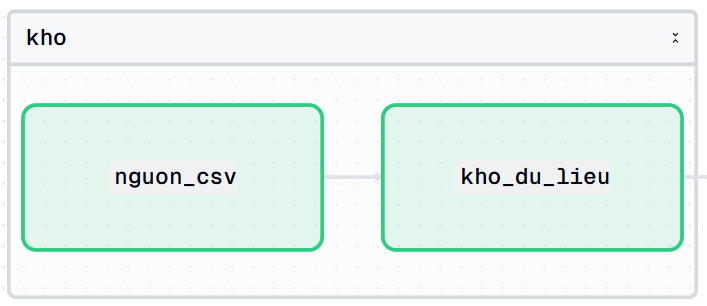
\includegraphics[width=0.62\textwidth]{image/dagster_1_kho.png}};
\node[dagimg, below=0.55cm of g1] (g2) {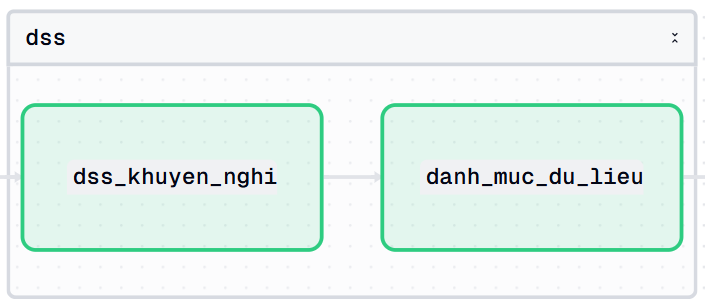
\includegraphics[width=0.62\textwidth]{image/dagster_1_dss.png}};
\node[dagimg, below=0.55cm of g2] (g3) {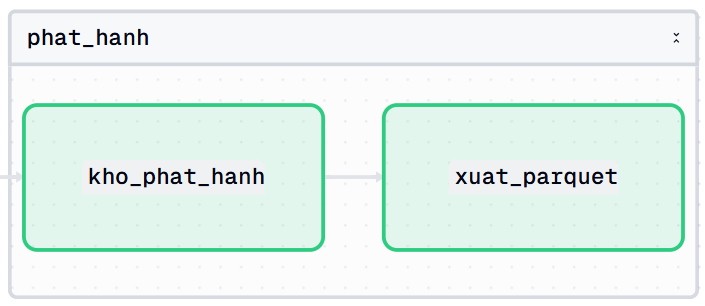
\includegraphics[width=0.62\textwidth]{image/dagster_1_phat_hanh.png}};
\draw[-{Stealth[length=2.6mm]}, line width=1pt, gray!70!black] (g1.south) -- (g2.north);
\draw[-{Stealth[length=2.6mm]}, line width=1pt, gray!70!black] (g2.south) -- (g3.north);
\end{tikzpicture}
\caption{Đồ thị phụ thuộc 6 asset trên Dagster (Global asset lineage), ba nhóm được xếp dọc để dễ đọc: kho $\rightarrow$ DSS $\rightarrow$ phát hành. Trong mỗi nhóm, asset bên trái chạy trước asset bên phải; viền xanh là đã chạy thành công}
\label{fig:dagster_lineage}
\end{figure}

Hình~\ref{fig:dagster_gantt} là biểu đồ Gantt của lần chạy job \texttt{dung\_lai\_toan\_bo} (mã \texttt{c0135898}), tương đương \emph{Gantt View} trong Airflow. Mỗi thanh là một bước, chiều dài là thời gian chạy:
\begin{itemize}
    \item Toàn bộ lần chạy mất \textbf{3 phút 14 giây}, cả \textbf{10/10 bước} thành công (6 asset và 4 kiểm tra), không bước nào lỗi.
    \item Bước dài nhất là \texttt{kho\_du\_lieu} (89 giây: dựng 26 đợt và lake), tiếp theo là kiểm tra \texttt{lakehouse\_va\_}\allowbreak\texttt{dbt} (38,5 giây, gồm test lakehouse và \texttt{dbt build}), \texttt{dss\_khuyen\_nghi} (18,6 giây: mô hình, MILP, đánh giá) và \texttt{kiem\_thu\_he\_thong} (15,5 giây).
    \item Hai kiểm tra \texttt{doi\_soat\_cac\_lop} và \texttt{bat\_thuong\_du\_lieu} chạy song song ngay sau khi kho dựng xong (khoảng 2 giây mỗi kiểm tra). Hai kiểm tra chặn \texttt{kiem\_thu\_he\_thong} và \texttt{lakehouse\_va\_dbt} cũng chạy song song; bước \texttt{kho\_phat\_hanh} (0,3 giây) chỉ bắt đầu khi cả hai đã đạt.
\end{itemize}
Lần chạy này phát hành bản kho \texttt{olist\_run\_c0135898.duckdb}. Bản này được đối chiếu với bản phát hành trước đó: số dòng và tổng tiền \texttt{fact\_sales\_item}, số phiên bản SCD2, số dòng cách ly, AUC và kế hoạch tại 01/07/2018 trùng khớp hoàn toàn, tức quy trình cho kết quả tái lập được (reproducible).

\appimage[0.98\textwidth]{image/dagster_4_run_gantt.png}{Biểu đồ Gantt lần chạy \texttt{dung\_lai\_toan\_bo} trên Dagster: 10 bước thành công trong 3 phút 14 giây}{fig:dagster_gantt}

Có ba job:
\begin{itemize}
    \item \texttt{dung\_lai\_toan\_bo}: chạy toàn bộ;
    \item \texttt{chay\_lai\_dss}: giữ kho, chép kho đang dùng kèm thư mục lake sang bản mới rồi chỉ tính lại DSS;
    \item \texttt{xuat\_power\_bi}: chỉ xuất lại Parquet.
\end{itemize}

\takeawaybox{Tóm tắt Chương 5}{
Ba lớp kiểm tra bổ sung cho nhau:
\begin{itemize}
    \item Đối soát theo đợt (286/286) bảo đảm không mất dòng, không lệch tiền giữa các lớp.
    \item Test hệ thống, test lakehouse và dbt bảo đảm cấu trúc đúng và hai cách dựng cho cùng kết quả.
    \item Cơ chế phát hành bảo đảm chỉ bản đã qua mọi kiểm tra mới tới tay người dùng.
\end{itemize}
Phép đối chiếu với dbt có giá trị thực tế: nó đã phát hiện một lỗi phình to dữ liệu (fan-out) với hệ số 4,56 mà các test của từng đường dựng riêng lẻ không bắt được.
}

    \newpage
    % !TEX root = ../main.tex
\section{OLAP VÀ GIAO DIỆN NGƯỜI DÙNG}
\suppressfloats[t]

Kho đã có dữ liệu và mô hình; câu hỏi tiếp theo là người dùng nhìn thấy gì. Chương này so sánh ROLAP và MOLAP trên cùng một kho, rồi giải thích vì sao Power BI dành cho người xem còn Streamlit dành cho người ra quyết định.

\subsection{Hai cách hiện thực OLAP trên cùng một kho}
\begin{table}[htbp]
\centering
\small
\caption{ROLAP và MOLAP trong hệ thống}
\label{tab:rolap_molap}
\begin{tabularx}{\textwidth}{|>{\raggedright\arraybackslash}m{2.4cm}|L|L|}
\hline
 & \textbf{ROLAP (DuckDB)} & \textbf{MOLAP (Power BI, chế độ Import)} \\
\hline
Nơi tính & SQL \texttt{GROUP BY}, \texttt{ROLLUP}, \texttt{CUBE} trên bảng Gold & Engine VertiPaq, dữ liệu nạp từ Parquet \\
\hline
Độ mới & Luôn là bản kho đang dùng & Bản chụp lúc xuất Parquet; phải bấm Làm mới \\
\hline
Ngữ nghĩa & Viết trong từng truy vấn & Semantic model: 50 measure DAX, quan hệ, hierarchy \\
\hline
Phân quyền & Không có & Row-level security theo vùng \\
\hline
Dùng ở & \texttt{src/sql/olap\_examples.sql}, Streamlit & 4 trang báo cáo cho R1, R2, R5 \\
\hline
\end{tabularx}
\end{table}

\subsubsection*{Tám truy vấn OLAP và thời gian chạy}
Bảng~\ref{tab:olap_time} đo thời gian trung bình của 5 lần chạy mỗi truy vấn trong \texttt{olap\_examples.sql}, trên bản kho đang dùng (DuckDB, máy thử nghiệm, kho đã nằm trong bộ nhớ đệm).

\begin{table}[htbp]
\centering
\small
\caption{Thời gian chạy tám truy vấn OLAP mẫu}
\label{tab:olap_time}
\begin{tabularx}{\textwidth}{|>{\raggedright\arraybackslash}m{2.3cm}|L|>{\raggedright\arraybackslash}m{3.5cm}|>{\raggedleft\arraybackslash}m{1.1cm}|>{\raggedleft\arraybackslash}m{1.3cm}|}
\hline
\textbf{Thao tác} & \textbf{Truy vấn} & \textbf{Đọc từ} & \textbf{Số dòng} & \textbf{ms} \\
\hline
ROLL-UP & GMV từ tháng lên quý, lên năm, kèm dòng tổng & \texttt{fact\_sales\_item} & 37 & 90,8 \\
\hline
DRILL-DOWN & Vùng $\rightarrow$ bang $\rightarrow$ seller, dùng dòng SCD2 có hiệu lực lúc mua & \texttt{fact\_sales\_item} & 20 & 11,3 \\
\hline
SLICE & Chỉ danh mục \texttt{housewares}: GMV và review theo tháng & \texttt{fact\_sales\_item} & 21 & 25,1 \\
\hline
DICE & Khách ở SP, quý 4/2017, đơn giao trễ & \texttt{fact\_order} & 19 & 6,4 \\
\hline
PIVOT & GMV theo tháng $\times$ hạng sức khỏe lúc bán & \texttt{fact\_seller\_monthly} & 9 & 28,5 \\
\hline
CUBE & KPI tính sẵn: tổng theo vùng của một tháng & \texttt{mart.kpi\_monthly} & 4 & 2,7 \\
\hline
SCD2 & Phân bố hạng tại một thời điểm trong quá khứ & \texttt{dim\_seller} & 7 & 1,8 \\
\hline
ROLE-PLAYING & Một \texttt{dim\_date} cho ngày mua và ngày giao: đơn Black Friday 2017 & \texttt{fact\_order} & 1 & 3,9 \\
\hline
\end{tabularx}
\end{table}

Truy vấn đọc bảng tính sẵn (\texttt{CUBE} trên \texttt{mart.kpi\_monthly}, 2,7 ms) nhanh hơn khoảng 34 lần so với ROLL-UP quét \texttt{fact\_sales\_item} (90,8 ms). Ở quy mô 112.650 dòng hàng, cả tám truy vấn đều dưới 0,1 giây, nên người dùng không cảm nhận được khác biệt. Lý do chính để giữ \texttt{kpi\_monthly} vì vậy \emph{không phải} tốc độ, mà là để có \textbf{số chốt sổ}: mỗi tháng được đóng băng lúc đóng đợt và không đổi khi dữ liệu sau này đến (Chương IV).

\subsection{Chia vai: Power BI cho người xem, Streamlit cho người ra quyết định}
Phân chia này đi theo bảng vai trò ở Chương I. Ban điều hành (R1) và quản lý vùng (R2) chỉ cần xem và lọc, nhưng cần phân quyền theo vùng; Power BI đáp ứng bằng RLS. Trưởng nhóm Seller Success (R3) lại cần giải lại bài toán tối ưu khi đổi ràng buộc, kéo thả để chỉnh tay và lưu kịch bản — những việc DAX không làm được và báo cáo Power BI không ghi lại thao tác người dùng. Vì thế phần này nằm ở Streamlit.

\subsubsection*{Power BI: 4 trang và phân quyền}
Asset \texttt{xuat\_parquet} xuất 12 bảng từ bản kho đang dùng: 7 dimension, 3 fact, \texttt{kpi\_monthly}, \texttt{dss\_recommendation}. Kèm theo là tệp \texttt{ke\_hoach\_da\_chot.parquet} do ứng dụng ghi khi người dùng chốt kế hoạch. Mô hình TMDL trong \texttt{powerbi/} gồm 4 trang (Bảng~\ref{tab:pbi_pages}).

\begin{table}[htbp]
\centering
\small
\caption{Bốn trang Power BI}
\label{tab:pbi_pages}
\begin{tabularx}{\textwidth}{|>{\raggedright\arraybackslash}m{3.2cm}|>{\centering\arraybackslash}m{1.3cm}|L|>{\centering\arraybackslash}m{1.4cm}|}
\hline
\textbf{Trang} & \textbf{Visual} & \textbf{Câu hỏi} & \textbf{Vai trò} \\
\hline
KPI tháng & 13 & GMV, đơn, seller có bán, trễ hẹn, review theo tháng; số chốt sổ & R1, R2 \\
\hline
Doanh số dồn ở đâu? & 11 & Cây phân rã vùng $\rightarrow$ bang $\rightarrow$ danh mục $\rightarrow$ hạng (drill-down, roll-up, slice, dice, pivot) & R1, R2 \\
\hline
Giao hàng & 11 & Trễ do seller hay do vận chuyển, theo tuyến & R5 \\
\hline
Kế hoạch & 14 & Kế hoạch đề xuất hoặc đã chốt, GMV rủi ro được xử lý & R1, R2 \\
\hline
\end{tabularx}
\end{table}

Role \texttt{Quản lý vùng Sudeste} lọc bảng \texttt{dim\_region} theo \texttt{region = "Sudeste"}. Bộ lọc lan qua \texttt{dim\_seller} tới mọi fact theo seller và tới \texttt{kpi\_monthly}. Trong DuckDB, Sudeste có 2.287 seller; số liệu Power BI dưới role này được đối chiếu với truy vấn DuckDB tương ứng. Hiện chỉ có một role làm mẫu. Các vùng khác dùng cùng mẫu nhưng chưa được tạo.

Hình~\ref{fig:pbi_kpi} tóm tắt bốn trang Power BI; Hình~\ref{fig:pbi_rls} mô tả cơ chế RLS — không phải ảnh chụp giao diện, mà là sơ đồ để đọc đúng phạm vi dữ liệu của từng trang.

\begin{figure}[htbp]
\centering
\begin{tikzpicture}[font=\erdfont\scriptsize]
\kcard[minimum height=1.9cm]{p1}{0,0}{hcmutnavy}{6.4cm}{kchart}{KPI tháng \textperiodcentered{} 13 visual}{GMV, đơn, seller, trễ hẹn, review theo tháng; số chốt sổ}
\kcard[minimum height=1.9cm]{p2}{6.9,0}{hcmutnavy}{6.4cm}{kchart}{Doanh số dồn ở đâu? \textperiodcentered{} 11 visual}{Cây phân rã vùng $\rightarrow$ bang $\rightarrow$ danh mục $\rightarrow$ hạng}
\kcard[minimum height=1.9cm]{p3}{0,-2.25}{hcmutnavy}{6.4cm}{kchart}{Giao hàng \textperiodcentered{} 11 visual}{Trễ do seller hay do vận chuyển, theo tuyến}
\kcard[minimum height=1.9cm]{p4}{6.9,-2.25}{hcmutnavy}{6.4cm}{kchart}{Kế hoạch \textperiodcentered{} 14 visual}{Kế hoạch đề xuất hoặc đã chốt, GMV rủi ro được xử lý}
\end{tikzpicture}
\caption{Sơ đồ bốn trang Power BI: mỗi trang trả lời một câu hỏi và dùng chung semantic model 50 measure; màu nền chỉ cùng một vai trò người xem}
\label{fig:pbi_kpi}
\end{figure}

\begin{figure}[htbp]
\centering
\begin{tikzpicture}[font=\erdfont\scriptsize]
\kcard[minimum height=1.9cm]{reg}{0,0}{kdss}{3.8cm}{kfilter}{Bộ lọc}{\texttt{dim\_region}\\ \texttt{region = "Sudeste"}}
\kcard[minimum height=1.9cm]{sel}{4.8,0}{kdss}{3.8cm}{kstar}{\texttt{dim\_seller}}{2.287 seller\\ thuộc Sudeste}
\kcard[minimum height=1.9cm]{fact}{9.6,0}{kdss}{3.8cm}{kdb}{Fact \& KPI}{\texttt{fact\_*} và \texttt{kpi\_monthly}\\ chỉ còn dòng Sudeste}
\draw[karrow] (reg.east) -- (sel.west);
\draw[karrow] (sel.east) -- (fact.west);
\node[anchor=north west, font=\erdfont\tiny, text=ksrc] at (0,-2.15) {Role mẫu hiện có một vùng; các vùng khác dùng cùng mẫu nhưng chưa tạo.};
\end{tikzpicture}
\caption{Cơ chế RLS: mũi tên đi từ lọc (\texttt{dim\_region}) sang lan (\texttt{dim\_seller}) rồi tới fact; số seller Sudeste 2.287 khớp truy vấn DuckDB}
\label{fig:pbi_rls}
\end{figure}


\subsubsection*{Streamlit: 5 màn, 2 luồng}
Mọi màn có một bộ chọn \textbf{mốc as-of} ở sidebar: người dùng ``tua thời gian'' và mọi màn chỉ thấy dữ liệu trước mốc đó. Các hình dưới đây chụp ở mốc 01/07/2018 với tham số mặc định.

\annotatedimage{image/app_1_can_chu_y_crop.png}{Luồng A, bước 1 -- Cần chú ý tháng này (mốc 01/07/2018). \uiref{1} Thẻ chỉ số rủi ro và kế hoạch; \uiref{2} danh sách seller mới vào Nguy cơ; \uiref{3} lý do seller chưa được xử lý; \uiref{4} GMV rủi ro theo hành động}{fig:ui_attention}{%
  \uimark{0.012}{0.90}{1}
  \uimark{0.010}{0.69}{2}
  \uimark{0.700}{0.69}{3}
  \uimark{0.700}{0.41}{4}}

\textbf{Màn Cần chú ý} (Hình~\ref{fig:ui_attention}) trả lời câu hỏi: seller nào \emph{vừa} rơi vào nhóm Nguy cơ. Thẻ chỉ số \uiref{1} cho biết tại 01/07/2018 có 70 seller mới vào Nguy cơ (tổng 89 seller đang ở hạng này); tổng GMV rủi ro 45 ngày của toàn sàn là 479 nghìn BRL, trong đó 70 seller mới đóng góp 29 nghìn BRL, và kế hoạch đề xuất xử lý 138 nghìn BRL qua 32 seller.

Bảng \uiref{2} xếp 70 seller theo GMV rủi ro, kèm khả năng sụt, số ngày chưa bán, tỷ lệ giao vận chuyển trễ và hành động được đề xuất. Biểu đồ \uiref{3} giải thích vì sao phần lớn các seller này \emph{không} được gọi: chỉ 2/70 seller nằm trong kế hoạch; 52 seller ngoài top 20\% GMV; 14 seller bị loại vì hết ngân sách hoặc hết suất; 2 seller dưới ngưỡng rủi ro 30\%. Cuối màn, \uiref{4} phân bổ GMV rủi ro của toàn bộ seller đang bán theo bốn nhóm hành động. Màn này cho thấy hạng (luật mô tả) và kế hoạch (tối ưu) là hai thứ khác nhau, và cho người dùng biết lý do chênh lệch giữa hai thứ đó.

\annotatedimage{image/app_2_chi_tiet_seller_crop.png}{Luồng A, bước 2 -- Chi tiết seller: chẩn đoán khâu gây sụt. \uiref{1} Thẻ chỉ số; \uiref{2} khuyến nghị và chẩn đoán; \uiref{3} GMV theo tháng; \uiref{4} đóng góp của từng feature vào xác suất sụt; \uiref{5} lịch sử SCD2 và mini-dimension}{fig:ui_seller}{%
  \uimark{0.010}{0.885}{1}
  \uimark{0.008}{0.745}{2}
  \uimark{0.010}{0.665}{3}
  \uimark{0.010}{0.305}{4}
  \uimark{0.388}{0.305}{5}}

\textbf{Màn Chi tiết seller} (Hình~\ref{fig:ui_seller}) chẩn đoán một seller. Với seller \texttt{7d13fca1} (SP), GMV 90 ngày là 62.232 BRL với 349 đơn, nhưng GMV tháng gần nhất thấp hơn bình quân 3 tháng liền trước 65\% (theo trend 90 ngày của mô hình là −54\%). Khả năng sụt GMV là 97\%; 18\% sản phẩm được bàn giao cho vận chuyển trễ hạn, và trung bình 3 tháng seller mất 4,2 ngày để bàn giao, vận chuyển mất 14,9 ngày.

Vì tỷ lệ bàn giao trễ vượt ngưỡng 15\%, hệ thống chẩn đoán lỗi ở khâu seller và đề xuất \texttt{OPS} thay vì \texttt{CALL}. Biểu đồ ``Vì sao khả năng sụt GMV 97\%'' tách log-odds thành đóng góp của từng feature (Chương VII). Đóng góp lớn nhất là cặp \emph{số đơn 90 ngày cao} (+) và \emph{số đơn 30 ngày} (−). Mô hình do đó nhận diện được mẫu hình seller có quy mô lớn nhưng suy giảm mạnh trong tháng gần nhất. Hai thẻ cuối hiển thị lịch sử SCD2 (3 phiên bản) và hồ sơ mini-dimension theo tháng của seller này.

\annotatedimage{image/app_3_bang_ke_hoach_crop.png}{Luồng A, bước 3 -- Bảng kế hoạch: bộ tối ưu đề xuất, người dùng kéo thả để chỉnh. \uiref{1} Ràng buộc và tham số; \uiref{2} kết quả kế hoạch; \uiref{3} đường cong ngân sách; \uiref{4} bốn cột hành động kéo thả; \uiref{5} chi tiết seller, Xuất CSV, Chốt kế hoạch}{fig:ui_board}{%
  \uimark{0.008}{0.955}{1}
  \uimark{0.008}{0.80}{2}
  \uimark{0.727}{0.80}{3}
  \uimark{0.008}{0.655}{4}
  \uimark{0.775}{0.20}{5}}

\textbf{Màn Bảng kế hoạch} (Hình~\ref{fig:ui_board}) là nơi ra quyết định. \uiref{1} Bốn thanh trượt là ràng buộc và tham số: ngân sách, số suất, ngưỡng rủi ro, top giá trị. Mỗi lần đổi, bộ tối ưu giải lại và cho ra một danh sách seller mới, không chỉ một con số mới.

\uiref{2} Ở cấu hình mặc định, kế hoạch dùng hết 2.000 BRL và 36/40 suất cho 28 seller \texttt{CALL} và 4 seller \texttt{OPS}. Kế hoạch bao phủ 138 nghìn trên tổng 378 nghìn BRL GMV rủi ro của các seller vượt ngưỡng; GMV giữ được kỳ vọng là 37 nghìn BRL (P10--P90: 28--46 nghìn). \uiref{3} Biểu đồ góc phải cho thấy chi trên khoảng 2.500 BRL gần như không thêm lợi ích (phân tích ở Chương VII). \uiref{4} Mỗi cột là một hành động; thẻ seller có thể kéo giữa các cột. \uiref{5} Bảng bên phải hiển thị chẩn đoán của seller đang chọn cùng hai nút Xuất CSV và Chốt kế hoạch.

Người dùng có thể kéo thẻ giữa các cột. Hình~\ref{fig:ui_drag} và Hình~\ref{fig:ui_violate} (Phụ lục B) chụp ở mốc 01/03/2018; đề xuất gốc tại mốc này là 16 seller \texttt{CALL} và 8 seller \texttt{OPS}. Khi kéo một seller khỏi cột \texttt{CALL} (Hình~\ref{fig:ui_drag}), tiền dùng giảm từ 2.000 xuống 1.950 BRL, suất dùng còn 31/40, GMV giữ được kỳ vọng thấp hơn đề xuất 1.116 BRL; hệ thống ghi ``Đã đổi 1 seller so với đề xuất, vẫn trong ràng buộc''. Khi chuyển một seller từ \texttt{CALL} sang \texttt{OPS} (Hình~\ref{fig:ui_violate}), tiền dùng thành 2.100 BRL; hệ thống cảnh báo ``Vượt ngân sách 100 BRL'' và khóa nút Chốt kế hoạch. Người dùng được quyền sửa đề xuất nhưng không thể chốt một kế hoạch vượt ràng buộc. Nút \textbf{Chốt kế hoạch} ghi kế hoạch cuối cùng, gồm cả thao tác tay, ra Parquet để Power BI đọc; nút \textbf{Xuất CSV} tạo danh sách cho nhân viên (R4).





\textbf{Màn Kiểm chứng} (Hình~\ref{fig:ui_validation}, Phụ lục B) đặt kế hoạch của các tháng trước cạnh kết quả thật 45 ngày sau. Phân tích chi tiết ở Chương VIII. Màn này cố ý hiển thị cả chỉ số mà DSS thua (bao phủ GMV mất thấp hơn cách chọn theo GMV ở 4/5 tháng), để người dùng không tin kế hoạch nhiều hơn mức số liệu cho phép.


\textbf{Màn What-if hẹn giao theo tuyến} (Hình~\ref{fig:ui_whatif}, Phụ lục B) phục vụ quản lý vận hành (R5). Với một tuyến, lấy các đơn mua từ 180 đến 60 ngày trước mốc (để mọi đơn đã kịp giao). Nếu hứa thêm $n$ ngày, tỷ lệ trễ được ước lượng bằng:
\begin{equation}
\text{late}(n) = \frac{1}{N} \sum_{o=1}^{N} \mathbb{I}(\text{delay\_days}_o > n)
\end{equation}
trong đó $\text{delay\_days}_o$ là số ngày nhận hàng muộn so với ngày hẹn (âm nếu sớm). Số ngày cần hứa thêm để đạt mục tiêu $\tau$ là $n^* = \min\{n : \text{late}(n) \le \tau\}$. Kết quả ở mốc 01/07/2018 với $\tau = 5\%$:
\begin{itemize}
    \item \textbf{SP$\rightarrow$SP} (9.052 đơn, lời hẹn trung bình 18,5 ngày): trễ 5,0\%, đạt mục tiêu chỉ với $n^* = +1$ ngày.
    \item \textbf{SP$\rightarrow$RJ} (2.338 đơn, lời hẹn 28,6 ngày): trễ 24,7\%. Hứa thêm 5 ngày còn 18,9\%, thêm 10 ngày còn 12,5\%, và cần $n^* = 23$ ngày. 86,0\% đơn trễ trên tuyến này có seller bàn giao đúng hạn.
    \item \textbf{SP$\rightarrow$CE} (283 đơn): trễ 32,5\%, cần 28 ngày; 91,3\% đơn trễ có seller đúng hạn.
\end{itemize}
Màn này dựa trên một giả định quan trọng: thời gian giao thực tế không đổi khi lời hẹn đổi. Nó cũng không đo được việc hứa lâu hơn làm mất bao nhiêu đơn. Với SP$\rightarrow$RJ, kết luận hợp lý là nới lời hẹn \emph{không} đủ (lời hẹn 51,6 ngày là không thực tế), và vấn đề cần chuyển sang đối tác vận chuyển. Đây đúng là loại quyết định mà R5 cần hỗ trợ.

\takeawaybox{Tóm tắt Chương VI}{
\begin{itemize}
    \item Power BI (MOLAP, có RLS) phục vụ người xem; Streamlit phục vụ người ra quyết định. Cả hai đọc cùng một bản kho đã phát hành.
    \item Hai giao diện được nối bằng kế hoạch đã chốt: quyết định của R3 trên Streamlit chảy sang trang Kế hoạch của Power BI cho R1, R2.
    \item Streamlit hiện chưa có đăng nhập. Quyền truy cập dựa vào việc ai có đường dẫn, và RLS mới có một vùng. Đây là giới hạn đã biết (Chương IX).
\end{itemize}
}

    \newpage
    % !TEX root = ../main.tex
\section{THIẾT KẾ VÀ HIỆN THỰC HỆ HỖ TRỢ QUYẾT ĐỊNH}
\suppressfloats[t]

Chương 6 đã chỉ ra nơi người dùng ra quyết định; chương này mô tả điều gì xảy ra phía sau nút bấm. Bốn phân hệ — dữ liệu, mô hình, giao diện, tri thức — được nối theo bốn pha của Simon, từ chấm điểm seller đến kế hoạch tối ưu và vòng kiểm chứng.

\subsection{Cấu trúc DSS và bốn pha Simon}
DSS gồm bốn phân hệ:
\begin{itemize}
    \item \textbf{Dữ liệu:} kho ở Chương 4--5;
    \item \textbf{Mô hình:} \texttt{src/dss/} gồm hồi quy logistic, bảng luật, MILP và Monte Carlo;
    \item \textbf{Giao diện:} Chương 6;
    \item \textbf{Tri thức:} luật phân hạng, lý do bằng chữ, định nghĩa KPI trong \texttt{metrics.yml}.
\end{itemize}
Bảng~\ref{tab:simon} gắn từng pha của Simon với dữ liệu và kết quả của luồng A.

\begin{table}[htbp]
\centering
\small
\caption{Bốn pha Simon trong luồng A (giữ chân seller)}
\label{tab:simon}
\begin{tabularx}{\textwidth}{|>{\raggedright\arraybackslash}m{2.2cm}|>{\raggedright\arraybackslash}m{2.6cm}|L|L|}
\hline
\textbf{Pha} & \textbf{Màn hình} & \textbf{Dữ liệu và mô hình} & \textbf{Kết quả ra} \\
\hline
Intelligence & Cần chú ý & \texttt{mart.seller\_features}, hạng tháng, \texttt{dss.scores} & Seller mới vào Nguy cơ, xếp theo GMV rủi ro \\
\hline
Design & Chi tiết seller & \texttt{fact\_seller\_monthly}, \texttt{fact\_order\_seller}, \texttt{dss.explain} & Chẩn đoán: lỗi khâu seller (\texttt{OPS}) hay giảm cầu (\texttt{CALL}) \\
\hline
Choice & Bảng kế hoạch & MILP trên \texttt{dss.scores} với tham số người dùng & Kế hoạch tối ưu, chỉnh tay, kịch bản, CSV \\
\hline
Implementation & Kiểm chứng; Power BI Kế hoạch & \texttt{dss.eval\_lists}, \texttt{dss.sensitivity}, kế hoạch đã chốt & Điều chỉnh ngưỡng, ngân sách cho tháng sau \\
\hline
\end{tabularx}
\end{table}

Hình~\ref{fig:influence} là sơ đồ ảnh hưởng (influence diagram) của bài toán. Mô hình có ba loại biến:
\begin{itemize}
    \item \textbf{Biến quyết định:} hành động cho từng seller.
    \item \textbf{Biến không kiểm soát được:} seller có sụt thật hay không, và hiệu quả thật của can thiệp.
    \item \textbf{Biến kết quả:} GMV giữ được, tiền dùng, suất dùng.
\end{itemize}

\begin{figure}[htbp]
\centering
\resizebox{0.95\textwidth}{!}{% Hình 7.1 -- Sơ đồ ảnh hưởng của bài toán phân bổ can thiệp
\begin{tikzpicture}[
  font=\erdfont\scriptsize,
  dec/.style={rectangle, draw=kdss, fill=kdss!9, line width=1pt, minimum height=0.95cm, align=center, inner sep=5pt, kshadow},
  unc/.style={ellipse, draw=kwarn, fill=kwarn!9, line width=1pt, align=center, inner sep=2pt, kshadow},
  res/.style={rectangle, rounded corners=9pt, draw=klake, fill=klake!9, line width=1pt, minimum height=0.95cm, align=center, inner sep=5pt, kshadow},
  par/.style={rectangle, rounded corners=2pt, draw=ksrc!55, fill=ksrc!6, line width=0.7pt, align=center, inner sep=5pt, kshadow},
  arr/.style={-{Stealth[length=5pt,width=4.5pt]}, line width=0.9pt, draw=ksrc!75}
]
\node[par] (feat) at (0,0) {\textbf{Feature tại as-of}\\\texttt{mart.seller\_features}};
\node[unc] (p) at (3.7,0) {\textbf{Khả năng sụt} $p_i$\\(hồi quy logistic)};
\node[par] (val) at (0,-1.7) {\textbf{Giá trị} $V_i = \text{GMV}_{90}/2$};
\node[par] (thr) at (0,1.7) {\textbf{Ngưỡng} rủi ro 0,30\\top 20\% giá trị};
\node[dec] (cand) at (3.7,1.7) {\textbf{Tập ứng viên} $C$};
\node[par] (res) at (7.4,2.8) {\textbf{Nguồn lực}: ngân sách $B$, số suất $S$\\chi phí, số suất mỗi hành động};
\node[dec] (act) at (7.4,1.05) {\textbf{Hành động} $x_{i,a}$\\(MILP)};
\node[unc] (eff) at (7.4,-1.05) {\textbf{Hiệu quả} $e(a)$\\(tham số giả định)};
\node[res] (out) at (11.2,0) {\textbf{GMV giữ được}\\$\sum p_i V_i\, e(a)\, x_{i,a}$};
\node[res] (cost) at (11.2,2.0) {\textbf{Tiền dùng, suất dùng}};
\draw[arr] (feat) -- (p);
\draw[arr] (thr) -- (cand); \draw[arr] (p) -- (cand); \draw[arr] (val) -- (cand);
\draw[arr] (cand) -- (act); \draw[arr] (res) -- (act);
\draw[arr] (act) -- (out); \draw[arr] (eff) -- (out); \draw[arr] (p) -- (out);
\draw[arr] (val.east) -- ++(0.4,0) |- ($(eff.south)+(0,-0.5)$) -| (out.south);
\draw[arr] (act) -- (cost);

% chú giải
\begin{scope}[shift={(0.3,-3.35)}, every node/.style={font=\erdfont\scriptsize}]
  \node[dec, minimum height=0.4cm, minimum width=0.7cm, inner sep=1pt] at (0,0) {};
  \node[anchor=west] at (0.5,0) {quyết định};
  \node[unc, minimum height=0.4cm, minimum width=0.8cm, inner sep=1pt] at (2.6,0) {};
  \node[anchor=west] at (3.1,0) {bất định};
  \node[res, minimum height=0.4cm, minimum width=0.7cm, inner sep=1pt, rounded corners=5pt] at (5.1,0) {};
  \node[anchor=west] at (5.6,0) {kết quả};
  \node[par, minimum height=0.4cm, minimum width=0.7cm, inner sep=1pt] at (7.5,0) {};
  \node[anchor=west] at (8.0,0) {tham số, dữ liệu};
\end{scope}
\end{tikzpicture}
}
\caption{Sơ đồ ảnh hưởng của bài toán phân bổ can thiệp}
\label{fig:influence}
\end{figure}

\subsection{Intelligence: feature và mô hình dự báo}
\subsubsection*{12 feature tại mốc as-of}
Mỗi feature chỉ dùng dữ liệu trước mốc $t$ (\texttt{mart.seller\_features}, Bảng~\ref{tab:features}). Hai biến tiền được biến đổi $\log(1+x)$; giá trị thiếu được thay bằng trung vị của tập huấn luyện; sau đó mọi biến được chuẩn hóa $z = (x - \mu)/\sigma$.

\begin{table}[htbp]
\centering
\small
\caption{Feature đầu vào và hệ số chuẩn hóa trung bình qua 13 mốc huấn luyện (\texttt{dss.model\_coef})}
\label{tab:features}
\begin{tabularx}{\textwidth}{|>{\raggedright\arraybackslash\ttfamily}m{3.1cm}|L|>{\raggedleft\arraybackslash}m{1.7cm}|>{\raggedleft\arraybackslash}m{1.7cm}|}
\hline
\textbf{\rmfamily Feature} & \textbf{\rmfamily Định nghĩa} & \textbf{\rmfamily $\beta$ decline} & \textbf{\rmfamily $\beta$ dormant} \\
\hline
orders\_30 & Số đơn 30 ngày & $-1{,}271$ & $-3{,}094$ \\
\hline
orders\_90 & Số đơn 90 ngày & $+0{,}701$ & $-0{,}892$ \\
\hline
recency & Số ngày từ đơn gần nhất tới $t$ & $+0{,}598$ & $+0{,}624$ \\
\hline
seller\_late\_rate & Tỷ lệ dòng hàng bàn giao trễ (đơn đã tới hạn) & $+0{,}180$ & $+0{,}212$ \\
\hline
trend & $\text{GMV}_{30}/(\text{GMV}_{90}/3) - 1$ & $+0{,}122$ & $+0{,}275$ \\
\hline
avg\_review & Review trung bình & $-0{,}100$ & $-0{,}076$ \\
\hline
cust\_late\_rate & Tỷ lệ đơn khách nhận trễ & $+0{,}093$ & $+0{,}087$ \\
\hline
days\_to\_carrier & Số ngày bàn giao trung bình & $-0{,}051$ & $-0{,}022$ \\
\hline
tenure & Số ngày từ đơn đầu tiên tới $t$ & $-0{,}042$ & $-0{,}069$ \\
\hline
gmv\_30 & $\log(1+\text{GMV}_{30})$ & $-0{,}042$ & $-0{,}042$ \\
\hline
gmv\_90 & $\log(1+\text{GMV}_{90})$ & $+0{,}033$ & $-0{,}145$ \\
\hline
n\_cat & Số danh mục đã bán & $+0{,}003$ & $-0{,}003$ \\
\hline
\end{tabularx}
\end{table}

\subsubsection*{Hồi quy logistic huấn luyện cuộn theo thời gian}
Với mỗi mục tiêu $y \in \{\text{decline}, \text{dormant}\}$:
\begin{equation}
p_i = P(y_i = 1 \mid z_i) = \sigma\!\left(\beta_0 + \sum_{j=1}^{12} \beta_j z_{ij}\right), \qquad \sigma(u) = \frac{1}{1 + e^{-u}}
\end{equation}
Mô hình tại mốc $t$ chỉ học từ các mốc $t' \le t - 45$ ngày, để nhãn của tập huấn luyện đã quan sát xong và không rò rỉ tương lai. Có 13 mốc được chấm điểm (09/2017--09/2018). Tập huấn luyện tăng từ 2.982 dòng (mốc 09/2017) lên 14.835 dòng (mốc 07/2018).

\textbf{Đọc hệ số (Bảng~\ref{tab:features}).} Ba biến mạnh nhất cho \texttt{decline} là \texttt{orders\_30} ($-1{,}27$), \texttt{orders\_90} ($+0{,}70$) và \texttt{recency} ($+0{,}60$). Khi giữ số đơn 90 ngày cố định, ít đơn trong 30 ngày gần nhất làm tăng rủi ro. Dấu dương của \texttt{orders\_90} không có nghĩa ``bán nhiều thì dễ sụt'': nó xuất hiện vì \texttt{orders\_90} và \texttt{orders\_30} tương quan mạnh, và mô hình đang đo \emph{độ giảm} từ 90 ngày về 30 ngày. Vì các biến tương quan với nhau, từng hệ số không được diễn giải như tác động nhân quả.

Các biến vận hành (\texttt{seller\_late\_rate}, \texttt{cust\_late\_rate}, \texttt{avg\_review}, \texttt{days\_to\_carrier}) có hệ số nhỏ. Chương 8 cho thấy bỏ chúng ra, AUC chỉ giảm 0,003--0,004. Hệ thống vẫn dùng các biến này, nhưng để \emph{chọn hành động} (\texttt{OPS} hay \texttt{CALL}), không phải để dự báo.

\subsubsection*{Giải thích từng dự báo}
Vì mô hình là tuyến tính trong log-odds, có thể tách đúng từng phần:
\begin{equation}
\log\frac{p_i}{1-p_i} = \underbrace{\beta_0}_{\text{hệ số chặn}} + \sum_{j} \underbrace{\beta_j z_{ij}}_{\text{đóng góp của feature } j}
\end{equation}
Bảng \texttt{dss.explain} lưu từng số hạng (230.451 dòng $= 13$ feature-hoặc-hệ-số-chặn $\times$ 17.727 cặp seller--mốc). Màn Chi tiết seller vẽ các số hạng này (Hình~\ref{fig:ui_seller}). Cộng mọi số hạng của một seller rồi qua hàm $\sigma$ thì được đúng $p_i$.

\subsection{Design: phân khúc và chọn hành động}
\texttt{src/dss/rules.py} gán phân khúc cho mỗi seller dựa trên ba cờ:
\begin{align}
\text{risk\_high}_i &= \mathbb{I}(p_i \ge 0{,}30) \\
\text{value\_high}_i &= \mathbb{I}(\text{GMV}_{90,i} \ge Q_{0{,}8}(\text{GMV}_{90})) \\
\text{ops\_poor}_i &= \mathbb{I}(\text{seller\_late\_rate}_i \ge 15\% \;\land\; n_{\text{đơn đã tới hạn}} \ge 5)
\end{align}
$Q_{0{,}8}$ là phân vị 80 của GMV 90 ngày trên các seller đang bán tại mốc đó (1.892,6 BRL tại 01/07/2018).

\begin{table}[htbp]
\centering
\small
\caption{Phân khúc, hành động khả dĩ và số seller tại mốc 01/07/2018 (1.658 seller)}
\label{tab:action_matrix}
\begin{tabularx}{\textwidth}{|>{\raggedright\arraybackslash}m{2.8cm}|L|>{\raggedright\arraybackslash}m{3.1cm}|>{\raggedleft\arraybackslash}m{1.9cm}|}
\hline
\textbf{Phân khúc} & \textbf{Điều kiện} & \textbf{Hành động} & \textbf{Số seller} \\
\hline
Giữ chân ngay & risk\_high $\land$ value\_high $\land$ $\neg$ops\_poor & \texttt{CALL} hoặc \texttt{OPS} qua MILP & 152 (28 được gọi) \\
\hline
Hỗ trợ vận hành & risk\_high $\land$ value\_high $\land$ ops\_poor & \texttt{CALL} hoặc \texttt{OPS} qua MILP & 35 (4 \texttt{OPS}) \\
\hline
Email tự động & risk\_high $\land$ $\neg$value\_high & \texttt{EMAIL} & 1.212 \\
\hline
Cảnh báo vận hành & $\neg$risk\_high $\land$ ops\_poor & \texttt{EMAIL} & 21 \\
\hline
Seller vàng & $\neg$risk\_high $\land$ value\_high $\land$ $\neg$ops\_poor & Không làm gì & 131 \\
\hline
Theo dõi & Còn lại & Không làm gì & 107 \\
\hline
\end{tabularx}
\end{table}

Chi phí, số suất và hiệu quả của từng hành động là \textbf{giả định} (Bảng~\ref{tab:assume}). Hiệu quả $e$ là tỷ lệ phần GMV đang có nguy cơ mất được giữ lại nếu seller thật sự sụt.

\begin{table}[htbp]
\centering
\small
\caption{Giả định chi phí và hiệu quả (\texttt{Params} trong \texttt{src/dss/rules.py})}
\label{tab:assume}
\begin{tabularx}{\textwidth}{|>{\raggedright\arraybackslash}m{2.6cm}|>{\centering\arraybackslash}m{1.8cm}|>{\centering\arraybackslash}m{1.4cm}|C|C|}
\hline
\textbf{Hành động} & \textbf{Chi phí (BRL)} & \textbf{Số suất} & \textbf{$e$ nếu vận hành tốt} & \textbf{$e$ nếu vận hành kém} \\
\hline
\texttt{CALL} & 50 & 1 & 20\% & 8\% \\
\hline
\texttt{OPS} & 150 & 2 & 5\% & 30\% \\
\hline
\texttt{EMAIL} & 0 & 0 & 3\% & 3\% \\
\hline
\end{tabularx}
\end{table}

Logic của bảng giả định: nếu seller trễ bàn giao, gọi điện kích cầu ít tác dụng (8\%) vì vấn đề nằm ở vận hành; ngược lại, hỗ trợ vận hành cho seller không có vấn đề vận hành gần như vô ích (5\%).

\subsubsection*{Bản chất và cách sử dụng các tham số hiệu quả}
Do bộ dữ liệu Olist không lưu trữ lịch sử can thiệp đối với seller, và trong phạm vi khảo sát tài liệu của đề tài chưa xác định được công bố nào cung cấp hệ số giữ chân seller cho sàn thương mại điện tử trung gian ở Brazil với định nghĩa ``sụt 50\% GMV trong 45 ngày'', các tham số hiệu quả 20\% (\texttt{CALL}) và 30\% (\texttt{OPS}) được thiết lập dưới dạng \textbf{tham số tiên nghiệm} (heuristic prior) do nhà quản trị xác định, không phải ước lượng thống kê. Theo đó, bài toán DSS đóng vai trò một \emph{khung phân tích độ nhạy} (sensitivity analysis framework) chứ không phải công cụ dự báo doanh thu. Cách tiếp cận này được bảo đảm bởi bốn cơ chế:
\begin{enumerate}
    \item \textbf{Tham số hóa minh bạch:} các giá trị nằm trong \texttt{Params} (\texttt{src/dss/rules.py}), hiển thị trên giao diện (nút Giả định) và người dùng R3 có thể thay bằng số liệu của chính tổ chức.
    \item \textbf{Chỉ có thứ tự tương đối là quan trọng với việc chọn seller:} khi mọi hiệu quả cùng nhân với một hệ số $\lambda > 0$, hàm mục tiêu (\ref{eq:milp_obj}) nhân với $\lambda$ nên tập seller tối ưu không đổi. Danh sách chỉ thay đổi khi \emph{tỷ lệ} hiệu quả giữa \texttt{CALL} và \texttt{OPS} thay đổi, và Chương 8 (Bảng~\ref{tab:sens}) đo mức thay đổi đó: khi hiệu quả \texttt{OPS} sai $\pm 50\%$, độ trùng Jaccard của danh sách vẫn đạt 0,82--0,83.
    \item \textbf{Định lượng bất định:} mô phỏng Monte Carlo (Mục 5) lan truyền sai số $\pm 25\%$ đến $\pm 75\%$ của tham số hiệu quả thành khoảng P10--P90 của GMV giữ được.
    \item \textbf{Lộ trình thay giả định bằng số đo:} thử nghiệm có nhóm đối chứng (Chương 9) cho phép ước lượng trực tiếp $e(a)$ sau khi hệ thống được vận hành.
\end{enumerate}
Do đó, mọi con số ``GMV giữ được'' trong báo cáo chỉ dùng để \emph{so sánh các phương án dưới cùng một bộ giả định}, không dùng để báo cáo doanh thu kỳ vọng tuyệt đối.

\subsection{Choice: tối ưu bằng quy hoạch nguyên}
Gọi $C$ là tập seller \texttt{risk\_high} $\land$ \texttt{value\_high}, $A = \{\texttt{CALL}, \texttt{OPS}\}$ là tập hành động và $V_i = \text{GMV}_{90,i}/2$ là GMV 45 ngày bình thường của seller $i$. Biến quyết định $x_{i,a} = 1$ nếu seller $i$ được giao hành động $a$, ngược lại bằng 0. Bài toán quy hoạch nguyên nhị phân (\texttt{src/dss/optimize.py}):
\begin{align}
\max_{x} \quad & \sum_{i \in C} \sum_{a \in A} \underbrace{p_i \, V_i \, e(a, \text{ops\_poor}_i)}_{g_{i,a}} \; x_{i,a} \label{eq:milp_obj} \\
\text{với} \quad & \sum_{i \in C} \sum_{a \in A} c_a \, x_{i,a} \le B = 2.000 \text{ BRL} \label{eq:milp_budget} \\
& \sum_{i \in C} \sum_{a \in A} s_a \, x_{i,a} \le S = 40 \text{ suất} \label{eq:milp_slot} \\
& \sum_{a \in A} x_{i,a} \le 1 \qquad \forall i \in C \label{eq:milp_one} \\
& x_{i,a} \in \{0, 1\} \qquad \forall i \in C,\; a \in A \label{eq:milp_bin}
\end{align}
Ràng buộc (\ref{eq:milp_bin}) là điều kiện nguyên nhị phân; thiếu nó, bài toán suy biến thành quy hoạch tuyến tính liên tục (LP) với nghiệm có thể ``gọi 0,4 seller''. Ràng buộc (\ref{eq:milp_budget}) và (\ref{eq:milp_slot}) là hai chiều tài nguyên, (\ref{eq:milp_one}) là ràng buộc chọn một. Đây là bài toán cái túi đa chiều (multi-dimensional knapsack) có ràng buộc chọn một, thuộc lớp NP-khó (Chương 2). Tại 01/07/2018, $|C| = 187$, nên bài toán có 374 biến nhị phân và $2 + 187 = 189$ ràng buộc. Bài toán được giải bằng HiGHS qua \texttt{scipy.optimize.milp} với giới hạn 10 giây; nếu bộ giải không chứng minh được tối ưu, \texttt{src/dss/optimize.py} phát cảnh báo kèm trạng thái và gap. Kiểm tra bằng \texttt{scripts/audit\_milp.py}, kết quả lưu ở \texttt{evidence/}\allowbreak\texttt{milp\_audit.json}, cho thấy cả 13 kế hoạch mặc định (114--502 biến) và 70 kế hoạch của phân tích độ nhạy đều kết thúc ở trạng thái \emph{Optimal}, gap bằng 0, lần giải lâu nhất dưới 0,15 giây. Như vậy giới hạn 10 giây chưa bao giờ bị chạm và mọi kế hoạch trong báo cáo là nghiệm tối ưu đã được chứng minh. Seller trong phân khúc Email tự động và Cảnh báo vận hành nhận \texttt{EMAIL}, vì hành động này có chi phí 0 nên không cần đưa vào bài toán.

\subsubsection*{Kết quả tại một mốc}
Tại 01/07/2018, nghiệm tối ưu chọn 28 \texttt{CALL} và 4 \texttt{OPS}. Chi phí là $28 \times 50 + 4 \times 150 = 2.000$ BRL, tức \textbf{ngân sách bị chặn}; số suất là $28 \times 1 + 4 \times 2 = 36 \le 40$, còn dư 4 suất. 32 seller được chọn đại diện cho 137.855 BRL GMV rủi ro ($p_i V_i$), bằng 36,5\% tổng GMV rủi ro của 1.399 seller vượt ngưỡng (377.524 BRL). GMV giữ được kỳ vọng là 32.459 BRL từ \texttt{CALL}/\texttt{OPS}, cộng 4.225 BRL từ 1.233 email, tổng \textbf{36.683 BRL}.

\subsubsection*{Kết quả qua 13 mốc}
\begin{figure}[htbp]
\centering
\begin{tikzpicture}
\begin{axis}[
    width=0.95\textwidth, height=5.6cm,
    ymin=0, ymax=420, ylabel={nghìn BRL},
    symbolic x coords={09/17,10/17,11/17,12/17,01/18,02/18,03/18,04/18,05/18,06/18,07/18,08/18,09/18},
    xtick=data, x tick label style={font=\footnotesize}, xlabel={Mốc as-of},
    legend style={at={(0.02,0.98)}, anchor=north west}, grid=major, grid style={gray!20},
]
\addplot[red!70!black, thick, mark=*, mark size=1.4pt] coordinates {(09/17,103.4) (10/17,131.1) (11/17,152.4) (12/17,129.8) (01/18,282.3) (02/18,288.7) (03/18,233.0) (04/18,246.3) (05/18,262.7) (06/18,309.9) (07/18,377.5) (08/18,340.5) (09/18,378.6)};
\addlegendentry{GMV rủi ro của seller vượt ngưỡng}
\addplot[hcmutnavy, thick, mark=square*, mark size=1.4pt] coordinates {(09/17,42.3) (10/17,48.0) (11/17,52.6) (12/17,40.0) (01/18,97.6) (02/18,111.4) (03/18,80.5) (04/18,60.6) (05/18,78.1) (06/18,84.8) (07/18,137.9) (08/18,114.7) (09/18,89.9)};
\addlegendentry{GMV rủi ro trong kế hoạch (CALL, OPS)}
\end{axis}
\end{tikzpicture}
\caption{GMV rủi ro toàn bộ và phần kế hoạch xử lý qua 13 mốc, ngân sách cố định 2.000 BRL}
\label{fig:risk_over_time}
\end{figure}

Hình~\ref{fig:risk_over_time} cho thấy ngân sách luôn là ràng buộc chặt: kế hoạch dùng đúng 2.000 BRL ở cả 13 mốc, trong khi số suất chỉ dùng 32--39/40. Phần được xử lý tụt lại so với rủi ro: GMV rủi ro của seller vượt ngưỡng tăng 3,66 lần (từ 103 lên 379 nghìn BRL, do sàn có nhiều seller hơn), còn phần kế hoạch xử lý chỉ dao động 40--138 nghìn BRL; tỷ lệ bao phủ giảm từ 40,9\% (09/2017) xuống 23,7\% (09/2018). Đây là thông tin dành cho R1: với ngân sách cố định, phần rủi ro được xử lý giảm dần khi sàn lớn lên.

\subsubsection*{Đường cong ngân sách}
Giải lại bài toán với $B$ từ 0 đến 8.000 BRL, giữ nguyên mọi tham số khác (\texttt{budget\_curve}, mốc 01/07/2018, chỉ tính \texttt{CALL}/\texttt{OPS}):

\begin{figure}[htbp]
\centering
\begin{tikzpicture}
\begin{axis}[
    width=0.62\textwidth, height=5.2cm,
    xmin=0, xmax=8000, ymin=0, ymax=38000,
    xlabel={Ngân sách $B$ (BRL)}, ylabel={GMV giữ được kỳ vọng (BRL)},
    scaled ticks=false, grid=major, grid style={gray!20},
    xtick={0,1000,2000,3000,4000,5000,6000,7000,8000},
]
\addplot[hcmutnavy, very thick, mark=*, mark size=1.6pt] coordinates {(0,0) (1000,26294) (2000,32459) (3000,33575) (4000,33575) (5000,33575) (6000,33575) (7000,33575) (8000,33575)};
\node[font=\scriptsize, anchor=west] at (axis cs:1150,24800) {14 seller};
\node[font=\scriptsize, anchor=north west] at (axis cs:2150,31300) {32 seller};
\node[font=\scriptsize, anchor=north] at (axis cs:5500,32300) {35 seller, chặn bởi 40 suất};
\end{axis}
\end{tikzpicture}
\caption{GMV giữ được kỳ vọng theo ngân sách (mốc 01/07/2018, 40 suất)}
\label{fig:budget_curve}
\end{figure}

Lợi ích biên giảm nhanh (Hình~\ref{fig:budget_curve}). 1.000 BRL đầu tiên giữ được 26.294 BRL (26,3 BRL cho mỗi BRL chi) vì bộ tối ưu chọn các seller có $g_{i,a}/c_a$ cao nhất trước; 1.000 BRL thứ hai chỉ thêm 6.165 BRL (6,2 BRL/BRL); 1.000 BRL thứ ba thêm 1.116 BRL (1,1 BRL/BRL). Từ 3.000 BRL trở lên không thêm gì, vì 35 seller được chọn đã dùng hết 40 suất và số suất trở thành ràng buộc chặt. Kết luận cho R1: việc mở rộng hạn mức ngân sách vượt quá ngưỡng 3.000 BRL mang lại hiệu suất biên tế tiệm cận 0 do vướng phải điểm nghẽn năng lực nhân sự; kết luận này phụ thuộc vào giả định hiệu quả ở Bảng~\ref{tab:assume}.

\subsubsection*{Chọn ngưỡng rủi ro}
Ngưỡng $0{,}30$ được chọn trên giai đoạn 09/2017--02/2018, tách biệt với giai đoạn kiểm chứng 03--07/2018 ở Chương 8. Bảng~\ref{tab:threshold} là kết quả chạy lại \texttt{scripts/tune\_threshold.py} trên kho hiện tại (trung bình 6 mốc).

\begin{table}[htbp]
\centering
\small
\caption{Ảnh hưởng của ngưỡng rủi ro trên giai đoạn chọn tham số 09/2017--02/2018}
\label{tab:threshold}
\begin{tabularx}{\textwidth}{|>{\centering\arraybackslash}m{1.3cm}|C|C|C|C|C|}
\hline
\textbf{Ngưỡng} & \textbf{Số ứng viên} & \textbf{Seller được chọn} & \textbf{Tiền dùng (BRL)} & \textbf{Gọi trúng} & \textbf{Bao phủ GMV mất} \\
\hline
0,20 & 147,0 & 31,7 & 2.000 & 46,3\% & 21,0\% \\
\hline
0,25 & 118,2 & 32,0 & 2.000 & 48,7\% & 21,3\% \\
\hline
\textbf{0,30} & \textbf{86,5} & \textbf{31,0} & \textbf{2.000} & \textbf{52,8\%} & \textbf{19,5\%} \\
\hline
0,35 & 61,0 & 31,0 & 2.000 & 56,0\% & 17,7\% \\
\hline
0,40 & 42,7 & 27,7 & 1.900 & 59,6\% & 16,5\% \\
\hline
0,45 & 32,2 & 23,8 & 1.725 & 62,2\% & 14,8\% \\
\hline
0,50 & 23,8 & 19,7 & 1.433 & 65,5\% & 12,5\% \\
\hline
\end{tabularx}
\end{table}

Bảng~\ref{tab:threshold} cho thấy không có ngưỡng nào trội trên cả hai chỉ số: ngưỡng càng cao thì gọi trúng càng cao nhưng bao phủ GMV mất càng thấp. Từ 0,40 trở lên, số ứng viên không đủ để dùng hết ngân sách. Giữa 0,30 và 0,35, ngưỡng 0,35 gọi trúng cao hơn 3,2 điểm \% nhưng bao phủ thấp hơn 1,8 điểm \% và chỉ có 61,0 ứng viên so với 86,5. So với 0,25, ngưỡng 0,30 đổi 1,8 điểm \% bao phủ lấy 4,1 điểm \% gọi trúng. Chọn 0,30 vì vậy là phán đoán ưu tiên gọi trúng trong khi vẫn giữ bao phủ gần mức cao nhất, không phải ưu tiên bao phủ thuần túy; người dùng đổi được ngưỡng trên giao diện.

\subsection{Rủi ro: mô phỏng Monte Carlo}
Giá trị kỳ vọng che đi độ bất định. \texttt{src/dss/simulate.py} mô phỏng $N = 2.000$ lần với hai nguồn bất định:
\begin{itemize}
    \item Seller $i$ có sụt thật hay không: $D_i \sim \text{Bernoulli}(p_i)$, độc lập giữa các seller.
    \item Hiệu quả thật của từng loại hành động $k$: $E_k \sim \text{Triangular}\big(e_k(1-\delta),\, e_k,\, e_k(1+\delta)\big)$, dùng \emph{chung} cho mọi seller cùng loại (sai số của giả định hiệu quả mang tính hệ thống, tác động đồng thời lên mọi seller cùng loại hành động). Độ bất định mặc định $\delta = 0{,}5$.
\end{itemize}
\begin{equation}
\text{Giữ được}^{(r)} = \sum_{i \in \text{kế hoạch}} D_i^{(r)} \, V_i \, E_{k(i)}^{(r)}, \qquad r = 1, \dots, N
\end{equation}

\begin{table}[htbp]
\centering
\small
\caption{Phân phối GMV giữ được của kế hoạch mặc định tại 01/07/2018 (2.000 lần mô phỏng, BRL)}
\label{tab:mc}
\begin{tabularx}{\textwidth}{|>{\raggedright\arraybackslash}m{3.6cm}|C|C|C|C|}
\hline
\textbf{Độ bất định $\delta$} & \textbf{P10} & \textbf{P50} & \textbf{P90} & \textbf{Kỳ vọng} \\
\hline
$\pm 25\%$ & 28.906 & 36.618 & 44.365 & 36.683 \\
\hline
$\pm 50\%$ (mặc định) & 27.584 & 36.355 & 46.207 & 36.683 \\
\hline
$\pm 75\%$ & 25.529 & 36.227 & 48.969 & 36.683 \\
\hline
\end{tabularx}
\end{table}

Trung bình mẫu ở $\delta = 0{,}5$ là 36.745 BRL, lệch 0,2\% so với kỳ vọng giải tích 36.683 BRL. Đây là kiểm tra chéo giữa bộ mô phỏng và bộ tối ưu. Trung vị P50 gần như không đổi (36.618 BRL ở $\delta = 0{,}25$, 36.227 BRL ở $\delta = 0{,}75$), trong khi khoảng P10--P90 rộng ra khi $\delta$ tăng: từ 15.459 BRL ($\delta = 0{,}25$) lên 23.440 BRL ($\delta = 0{,}75$). Trong 2.000 lần mô phỏng, không lần nào giữ được ít hơn 2.000 BRL tiền chi. Điều này \textbf{không} chứng minh kế hoạch có lãi: nó chỉ là hệ quả của giả định hiệu quả, vì nếu hiệu quả thật gần 0 thì GMV giữ được cũng gần 0.

\subsection{Implementation: chốt, khép vòng và What-if}
Kế hoạch được chỉnh trên Bảng kế hoạch (Hình~\ref{fig:ui_board}), lưu thành kịch bản để so sánh, rồi chốt. Khi chốt, \texttt{src/app/decisions.py} ghi kế hoạch kèm thao tác tay ra \texttt{ke\_hoach\_da\_chot.parquet}. Power BI nối tệp này với \texttt{dim\_seller} và \texttt{dim\_date}, nên RLS theo vùng vẫn áp dụng; các measure ``(áp dụng)'' dùng bản đã chốt nếu mốc đó đã chốt, nếu không thì dùng đề xuất của MILP. Cơ chế này đưa quyết định thật của R3 tới R1 và R2. Đây là bước ``thực hiện và theo dõi'' của Simon. Power BI chỉ cập nhật khi bấm Làm mới, không phải thời gian thực.

Luồng B dùng công thức $\text{late}(n)$ ở Chương 6. Hai luồng gặp nhau ở màn Chi tiết seller: nếu \texttt{ops\_poor}, đề xuất \texttt{OPS} (luồng A); nếu trễ nằm ở vận chuyển, màn hình dẫn sang What-if tuyến (luồng B).

\takeawaybox{Tóm tắt Chương 7}{
\begin{itemize}
    \item DSS chuyển xác suất dự báo thành một kế hoạch cụ thể dưới hai ràng buộc. Ở cấu hình mặc định, ngân sách là ràng buộc chặt ở cả 13 mốc; quá khoảng 3.000 BRL thì số suất chặn.
    \item Mọi con số ``GMV giữ được'' (ví dụ 36.683 BRL, P10--P90 27.584--46.207 BRL tại 01/07/2018) phụ thuộc vào giả định hiệu quả chưa được kiểm chứng. Chúng dùng để \emph{so sánh phương án}, không dùng để báo cáo doanh thu.
\end{itemize}
}

    \newpage
    % !TEX root = ../main.tex
\section{KIỂM THỬ VÀ ĐÁNH GIÁ}
\suppressfloats[t]

Chương 7 đã trình bày cách hệ thống ra quyết định; câu hỏi còn lại là nó đúng đến đâu. Chương này kiểm thử hệ thống, đo khả năng xếp hạng của mô hình, kiểm chứng ngược kế hoạch trên năm tháng, và đo độ nhạy của kế hoạch trước các giả định.

\subsection{Kiểm thử tự động}
Bảng~\ref{tab:tests} tổng hợp các bộ kiểm thử trên bản kho đang phát hành. Ba bộ đầu và dbt là \emph{cổng phát hành}: chỉ cần một bộ hỏng là bản kho mới không được dùng (Chương 5).

\begin{table}[htbp]
\centering
\small
\caption{Các bộ kiểm thử và kết quả}
\label{tab:tests}
\begin{tabularx}{\textwidth}{|>{\raggedright\arraybackslash}m{4.3cm}|>{\centering\arraybackslash}m{1.6cm}|L|}
\hline
\textbf{Bộ kiểm thử} & \textbf{Kết quả} & \textbf{Kiểm tra gì} \\
\hline
Đối soát theo đợt (\texttt{13\_batch\_checks.sql}) & 286/286 & 11 phép đối soát số dòng, số tiền $\times$ 26 đợt \\
\hline
\texttt{tests/test\_system.py} & 133/133 & Hash nguồn, số dòng các lớp, khóa, SCD2, chống rò rỉ tương lai, tối ưu trên bài toán tính tay, mô phỏng, cổng chất lượng, catalog \\
\hline
\texttt{tests/test\_lakehouse\_\allowbreak medallion.py} & 11/11 & Đủ tệp Parquet, Parquet khớp kho, sổ cái, cách ly \\
\hline
\texttt{dbt build} & 79/79 & 27 model, 52 test gồm đối chiếu với kho chính \\
\hline
\texttt{tests/test\_release.py} & 15/15 & Phát hành khi app đang mở, quay lui, từ chối bản lỗi \\
\hline
\texttt{tests/test\_edges.py} & 65/65 & Mỗi màn hình $\times$ các mốc as-of và tổ hợp lọc biên, không lỗi \\
\hline
\texttt{tests/test\_ui.py} (trình duyệt thật) & 45/45 & Kéo thả, ràng buộc, xuất CSV, What-if, không cuộn trang \\
\hline
\end{tabularx}
\end{table}

Một số kịch bản kiểm thử trong \texttt{test\_system.py} được xây dựng theo tinh thần kiểm thử đột biến (mutation testing): chủ động tiêm lỗi vào hệ thống nhằm kích hoạt các trạng thái lỗi biên và xác nhận cơ chế phòng vệ phản ứng đúng:
\begin{itemize}
    \item Xóa 1 dòng ở \texttt{fact\_sales\_item} trên bản sao kho rồi chạy lại đợt cuối: đợt bị dừng, ghi \texttt{failed} kèm nội dung lỗi, và watermark không tiến.
    \item Chạy lại đợt cuối khi không có thay đổi: không bảng nào trong 15 bảng được kiểm có thêm dòng (idempotent).
    \item Kiểm tra chống rò rỉ tương lai:
    \begin{itemize}
        \item không đợt nào ở Bronze chứa ngày giao vận chuyển hoặc ngày nhận sau mốc chốt của đợt (0 dòng);
        \item không review nào vào kho trước khi khách trả lời (0 dòng);
        \item khoảng cách giữa mốc huấn luyện cuối và mốc chấm điểm nhỏ nhất là 59 ngày, đạt yêu cầu $\ge 45$ ngày.
    \end{itemize}
    \item Kiểm tra giải thích: cộng các số hạng trong \texttt{dss.explain} rồi qua hàm sigmoid phải ra đúng $p_{\text{decline}}$ đã lưu.
\end{itemize}
Kiểm thử trả lời câu hỏi ``hệ thống có làm đúng điều nó định làm không''. Nó không trả lời câu hỏi ``điều đó có đúng về nghiệp vụ không''. Câu hỏi thứ hai được xét ở các mục dưới.

\subsection{Khả năng xếp hạng của mô hình}
Mô hình được đánh giá trên 11 mốc có nhãn đầy đủ (09/2017--07/2018). Tại mỗi mốc, mô hình chỉ được huấn luyện trên các mốc trước đó ít nhất 45 ngày. Ngoài mô hình đầy đủ, có hai mô hình để so sánh:
\begin{itemize}
    \item \textbf{Bỏ biến vận hành:} logistic không có 4 biến vận hành;
    \item \textbf{Chỉ dùng recency:} xếp hạng seller theo số ngày chưa bán, không cần mô hình.
\end{itemize}

\begin{figure}[htbp]
\centering
\begin{tikzpicture}
\begin{axis}[
    width=0.95\textwidth, height=5.8cm,
    ymin=0.62, ymax=0.88, ylabel={AUC},
    symbolic x coords={09/17,10/17,11/17,12/17,01/18,02/18,03/18,04/18,05/18,06/18,07/18},
    xtick=data, x tick label style={font=\footnotesize}, xlabel={Mốc as-of},
    legend columns=2, legend style={at={(0.5,1.03)}, anchor=south}, grid=major, grid style={gray!20},
    /pgf/number format/precision=2,
]
\addplot[hcmutnavy, thick, mark=*, mark size=1.4pt] coordinates {(09/17,0.817) (10/17,0.839) (11/17,0.805) (12/17,0.825) (01/18,0.815) (02/18,0.843) (03/18,0.844) (04/18,0.841) (05/18,0.834) (06/18,0.803) (07/18,0.817)};
\addlegendentry{dormant: mô hình}
\addplot[hcmutnavy, dashed, mark=o, mark size=1.4pt] coordinates {(09/17,0.776) (10/17,0.771) (11/17,0.778) (12/17,0.788) (01/18,0.778) (02/18,0.796) (03/18,0.801) (04/18,0.798) (05/18,0.788) (06/18,0.772) (07/18,0.789)};
\addlegendentry{dormant: chỉ recency}
\addplot[red!70!black, thick, mark=square*, mark size=1.4pt] coordinates {(09/17,0.703) (10/17,0.719) (11/17,0.733) (12/17,0.697) (01/18,0.703) (02/18,0.742) (03/18,0.731) (04/18,0.705) (05/18,0.709) (06/18,0.674) (07/18,0.707)};
\addlegendentry{decline: mô hình}
\addplot[red!70!black, dashed, mark=square, mark size=1.4pt] coordinates {(09/17,0.683) (10/17,0.698) (11/17,0.715) (12/17,0.687) (01/18,0.708) (02/18,0.730) (03/18,0.726) (04/18,0.690) (05/18,0.691) (06/18,0.664) (07/18,0.697)};
\addlegendentry{decline: chỉ recency}
\end{axis}
\end{tikzpicture}
\caption{AUC theo mốc của mô hình và của cách xếp theo số ngày chưa bán (\texttt{dss.eval\_auc})}
\label{fig:auc}
\end{figure}

\begin{table}[htbp]
\centering
\small
\caption{AUC trung bình trên 11 mốc}
\label{tab:auc}
\begin{tabularx}{\textwidth}{|>{\raggedright\arraybackslash}m{2.4cm}|>{\centering\arraybackslash}m{2.4cm}|C|C|C|C|}
\hline
\textbf{Mục tiêu} & \textbf{Tỷ lệ dương} & \textbf{Mô hình đầy đủ (min--max)} & \textbf{Bỏ biến vận hành} & \textbf{Chỉ recency} & \textbf{Chênh so với recency} \\
\hline
\texttt{decline} & 35,6--51,1\% & 0,711 (0,674--0,742) & 0,708 & 0,699 & +0,012 \\
\hline
\texttt{dormant} & 26,6--33,5\% & 0,826 (0,803--0,844) & 0,822 & 0,785 & +0,041 \\
\hline
\end{tabularx}
\end{table}

Hình~\ref{fig:auc} và Bảng~\ref{tab:auc} cho thấy mô hình dự báo tạm ngừng tốt hơn rõ rệt so với dự báo sụt GMV: AUC trung bình 0,826 so với 0,711. Điều này có lý: không có đơn nào trong 45 ngày tới là hiện tượng gần với “đã lâu không bán”, còn sụt dưới 50\% phụ thuộc biến động nhu cầu khó đoán hơn. Tuy vậy, so với quy tắc đơn biến theo độ tươi mới giao dịch, mô hình 12 biến chỉ hơn 0,012 AUC ở mục tiêu \texttt{decline} — và còn thua ở 01/2018 (0,703 so với 0,708); với \texttt{dormant}, khoảng cách là 0,041 và mô hình hơn ở cả 11 mốc.

Bốn biến vận hành gần như không giúp dự báo: bỏ chúng đi, AUC chỉ giảm 0,003 (\texttt{decline}) và 0,004 (\texttt{dormant}). AUC cũng ổn định theo thời gian (độ lệch giữa các mốc dưới 0,07) dù tập huấn luyện tăng gấp 5 lần, từ 2.982 lên 14.835 dòng. Thêm dữ liệu không làm mô hình tốt lên rõ — giới hạn nằm ở feature, không ở cỡ mẫu.

Để kiểm tra giới hạn này nằm ở dữ liệu hay ở dạng mô hình, nhóm thử thay hồi quy logistic bằng gradient boosting (\texttt{HistGradientBoostingClassifier}, 200 cây), mô hình phi tuyến bắt được tương tác giữa các feature, với cùng 12 feature và cùng cách huấn luyện theo thời gian trên 11 mốc 09/2017--07/2018 (\texttt{scripts/compare\_models.py}). Gradient boosting đạt AUC trung bình 0,703, thấp hơn logistic (0,711), và Brier score kém hơn (0,220 so với 0,215). Xác suất của logistic cũng gần đúng mức: trung bình xác suất dự báo 0,39--0,45 so với tỷ lệ sụt thật 0,36--0,51. Vì vậy nhóm giữ logistic: mô hình phức tạp hơn không thêm khả năng xếp hạng, còn logistic cho phép tách chính xác đóng góp của từng feature để giải thích cho người dùng (Chương 7). Muốn dự báo tốt hơn thì cần feature mới (lượt xem, tồn kho, giá so với đối thủ), mà tập dữ liệu Olist không có.
\subsubsection*{Đường cong ROC và Precision-Recall tại mốc 01/07/2018}
AUC trung bình che mất hành vi của mô hình ở từng ngưỡng cắt. Hình~\ref{fig:roc_pr} vẽ đường cong ROC và Precision-Recall của mục tiêu \texttt{decline} tại mốc chuẩn 01/07/2018 (1.658 seller đang bán, tỷ lệ sụt thật 45,1\%), cho cả mô hình và quy tắc recency. Các điểm được tính trực tiếp từ \texttt{dss.scores}, \texttt{dss.labels} và \texttt{mart.seller\_features}; AUC tại mốc này là 0,707 (mô hình) và 0,697 (recency), độ chính xác trung bình (average precision) là 0,655 và 0,650.

\begin{figure}[htbp]
\centering
\begin{tikzpicture}
\begin{axis}[
    name=roc, width=0.49\textwidth, height=0.49\textwidth,
    xmin=0, xmax=1, ymin=0, ymax=1,
    xlabel={Tỷ lệ dương giả (FPR)}, ylabel={Tỷ lệ dương thật (TPR, recall)},
    title={\footnotesize (a) ROC -- \texttt{decline}},
    grid=major, grid style={gray!20},
    xtick={0,0.2,0.4,0.6,0.8,1}, ytick={0,0.2,0.4,0.6,0.8,1},
    xticklabels={0,{0,2},{0,4},{0,6},{0,8},1}, yticklabels={0,{0,2},{0,4},{0,6},{0,8},1},
    legend style={at={(0.97,0.03)}, anchor=south east, font=\tiny},
]
\addplot[gray, dashed] coordinates {(0,0) (1,1)};
\addlegendentry{Ngẫu nhiên (0,5)}
\addplot[hcmutnavy, thick] coordinates {(0.000,0.009) (0.025,0.122) (0.050,0.178) (0.075,0.248) (0.100,0.345) (0.125,0.373) (0.150,0.411) (0.175,0.455) (0.200,0.489) (0.225,0.537) (0.250,0.556) (0.275,0.581) (0.300,0.616) (0.325,0.632) (0.350,0.661) (0.375,0.676) (0.400,0.687) (0.425,0.701) (0.450,0.724) (0.475,0.747) (0.500,0.767) (0.525,0.786) (0.550,0.803) (0.575,0.826) (0.600,0.842) (0.625,0.859) (0.650,0.874) (0.675,0.884) (0.700,0.893) (0.725,0.898) (0.750,0.909) (0.775,0.920) (0.800,0.941) (0.825,0.950) (0.850,0.957) (0.875,0.972) (0.900,0.987) (0.925,0.989) (0.950,0.995) (0.975,1.000) (1.000,1.000)};
\addlegendentry{Mô hình (0,707)}
\addplot[red!70!black, thick, dash dot] coordinates {(0.000,0.005) (0.025,0.103) (0.050,0.191) (0.075,0.261) (0.100,0.316) (0.125,0.341) (0.150,0.384) (0.175,0.442) (0.200,0.474) (0.225,0.518) (0.250,0.544) (0.275,0.565) (0.300,0.597) (0.325,0.618) (0.350,0.627) (0.375,0.653) (0.400,0.671) (0.425,0.699) (0.450,0.726) (0.475,0.744) (0.500,0.767) (0.525,0.782) (0.550,0.797) (0.575,0.821) (0.600,0.834) (0.625,0.853) (0.650,0.867) (0.675,0.871) (0.700,0.886) (0.725,0.901) (0.750,0.914) (0.775,0.925) (0.800,0.930) (0.825,0.933) (0.850,0.949) (0.875,0.956) (0.900,0.964) (0.925,0.973) (0.950,0.985) (0.975,0.991) (1.000,1.000)};
\addlegendentry{Recency (0,697)}
\addplot[only marks, mark=*, mark size=2.4pt, color=orange!85!black] coordinates {(0.779,0.922)};
\node[font=\tiny, anchor=north west, align=left] at (axis cs:0.50,0.80) {ngưỡng $p \ge 0{,}30$\\(1.399 seller)};
\addplot[only marks, mark=diamond*, mark size=2.8pt, color=orange!85!black] coordinates {(0.204,0.491)};
\node[font=\tiny, anchor=west] at (axis cs:0.22,0.46) {$p \ge 0{,}50$ (553 seller)};
\end{axis}
\begin{axis}[
    at={(roc.east)}, anchor=west, xshift=1.3cm,
    width=0.49\textwidth, height=0.49\textwidth,
    xmin=0, xmax=1, ymin=0.3, ymax=1,
    xlabel={Recall}, ylabel={Precision (tỷ lệ gọi trúng)},
    title={\footnotesize (b) Precision-Recall -- \texttt{decline}},
    grid=major, grid style={gray!20},
    xtick={0,0.2,0.4,0.6,0.8,1},
    ytick={0.4,0.6,0.8,1}, xticklabels={0,{0,2},{0,4},{0,6},{0,8},1}, yticklabels={{0,4},{0,6},{0,8},1},
    legend style={at={(0.03,0.03)}, anchor=south west, font=\tiny},
]
\addplot[gray, dashed] coordinates {(0,0.451) (1,0.451)};
\addlegendentry{Tỷ lệ cơ sở (0,451)}
\addplot[hcmutnavy, thick] coordinates {(0.025,0.809) (0.050,0.809) (0.075,0.809) (0.100,0.809) (0.125,0.808) (0.150,0.792) (0.175,0.750) (0.200,0.749) (0.225,0.746) (0.250,0.746) (0.275,0.746) (0.300,0.746) (0.325,0.746) (0.350,0.740) (0.375,0.710) (0.400,0.699) (0.425,0.692) (0.450,0.685) (0.475,0.670) (0.500,0.667) (0.525,0.666) (0.550,0.653) (0.575,0.641) (0.600,0.631) (0.625,0.624) (0.650,0.609) (0.675,0.598) (0.700,0.579) (0.725,0.568) (0.750,0.563) (0.775,0.556) (0.800,0.546) (0.825,0.541) (0.850,0.531) (0.875,0.524) (0.900,0.501) (0.925,0.493) (0.950,0.487) (0.975,0.477) (1.000,0.459)};
\addlegendentry{Mô hình (AP 0,655)}
\addplot[red!70!black, thick, dash dot] coordinates {(0.025,0.913) (0.050,0.847) (0.075,0.826) (0.100,0.781) (0.125,0.765) (0.150,0.765) (0.175,0.765) (0.200,0.765) (0.225,0.757) (0.250,0.754) (0.275,0.729) (0.300,0.728) (0.325,0.711) (0.350,0.687) (0.375,0.683) (0.400,0.681) (0.425,0.681) (0.450,0.669) (0.475,0.664) (0.500,0.659) (0.525,0.651) (0.550,0.635) (0.575,0.624) (0.600,0.619) (0.625,0.602) (0.650,0.589) (0.675,0.578) (0.700,0.575) (0.725,0.570) (0.750,0.560) (0.775,0.558) (0.800,0.544) (0.825,0.538) (0.850,0.529) (0.875,0.515) (0.900,0.505) (0.925,0.495) (0.950,0.477) (0.975,0.462) (1.000,0.451)};
\addlegendentry{Recency (AP 0,650)}
\addplot[only marks, mark=*, mark size=2.4pt, color=orange!85!black] coordinates {(0.922,0.492)};
\addplot[only marks, mark=diamond*, mark size=2.8pt, color=orange!85!black] coordinates {(0.491,0.664)};
\node[font=\tiny, anchor=south] at (axis cs:0.49,0.68) {$p \ge 0{,}50$};
\node[font=\tiny, anchor=south] at (axis cs:0.88,0.51) {$p \ge 0{,}30$};
\end{axis}
\end{tikzpicture}
\caption[ROC và Precision-Recall của \texttt{decline} tại 01/07/2018]{Đường cong ROC (a) và Precision-Recall (b) của mục tiêu \texttt{decline} tại mốc 01/07/2018; điểm cam là các ngưỡng cắt trên xác suất dự báo (precision trong hình (b) được nội suy theo cực đại bên phải)}
\label{fig:roc_pr}
\end{figure}

Hình~\ref{fig:roc_pr} cho thấy hai đường ROC gần như chồng lên nhau, xác nhận ở cấp từng ngưỡng điều mà AUC trung bình đã chỉ ra: thông tin dự báo chủ yếu nằm ở độ tươi mới của giao dịch. Ở vùng đầu danh sách (recall dưới khoảng 7\%), recency còn cho precision cao hơn mô hình (0,78--0,91 so với 0,81); đến recall 10\% thì hai đường xấp xỉ nhau (0,781 so với 0,809).

Ngưỡng $p \ge 0{,}30$ là một điểm làm việc thiên về độ phủ: 1.399/1.658 seller vượt ngưỡng, recall 92,2\% nhưng precision chỉ 49,2\%, gần tỷ lệ cơ sở. Điều này có chủ đích, vì ngưỡng 0,30 chỉ là bộ lọc thô để tạo tập ứng viên; việc chọn ai trong số đó do bộ tối ưu quyết định theo $p_i V_i$ dưới ràng buộc ngân sách. Nếu nâng ngưỡng lên 0,50, precision tăng lên 66,4\% nhưng recall giảm còn 49,1\%. Precision của mô hình giảm đơn điệu theo recall và luôn nằm trên tỷ lệ cơ sở 0,451, tức mô hình có giá trị xếp hạng ở mọi ngưỡng, dù không vượt trội so với quy tắc recency.

Kết luận: giá trị của DSS \emph{không} nằm ở độ chính xác dự báo. Nếu nó tạo ra khác biệt, khác biệt đó phải đến từ cách chuyển xác suất thành lựa chọn dưới ràng buộc. Mục tiếp theo kiểm tra điều này.

\subsection{Kiểm chứng ngược kế hoạch trên 5 tháng}
Trên 5 mốc 03--07/2018 (không dùng để chọn tham số), so sánh hai danh sách \textbf{cùng số seller} $k$:
\begin{itemize}
    \item \textbf{Kế hoạch DSS:} các seller được MILP chọn \texttt{CALL} hoặc \texttt{OPS};
    \item \textbf{Theo GMV:} $k$ seller có $\text{GMV}_{90}$ lớn nhất, đây là cách làm phổ biến khi không có mô hình.
\end{itemize}
Hai chỉ số dùng nhãn thật 45 ngày sau mốc:
\begin{align}
\text{Gọi trúng} &= \frac{|\{i \in L : \text{decline}_i = 1\}|}{|L|} \\
\text{Bao phủ GMV mất} &= \frac{\sum_{i \in L} \text{loss}_i}{\sum_{i \in \text{mọi seller}} \text{loss}_i}
\end{align}

\begin{table}[htbp]
\centering
\small
\caption{Kế hoạch DSS và chọn theo GMV, cùng số seller (\texttt{dss.eval\_lists}, scope \texttt{plan})}
\label{tab:backtest_comparison}
\begin{tabularx}{\textwidth}{|>{\centering\arraybackslash}m{1.6cm}|>{\centering\arraybackslash}m{0.8cm}|>{\centering\arraybackslash}m{1.9cm}|C|C|C|C|}
\hline
\multirow{2}{*}{\textbf{Mốc}} & \multirow{2}{*}{$k$} & \multirow{2}{*}{\textbf{Tỷ lệ decline}} & \multicolumn{2}{c|}{\textbf{Gọi trúng}} & \multicolumn{2}{c|}{\textbf{Bao phủ GMV mất}} \\
\cline{4-7}
 & & & \textbf{DSS} & \textbf{GMV} & \textbf{DSS} & \textbf{GMV} \\
\hline
03/2018 & 24 & 44,2\% & 50,0\% & 20,8\% & 19,5\% & 23,7\% \\
\hline
04/2018 & 28 & 45,0\% & 64,3\% & 21,4\% & 17,0\% & 16,1\% \\
\hline
05/2018 & 32 & 48,5\% & 62,5\% & 31,3\% & 19,1\% & 24,4\% \\
\hline
06/2018 & 36 & 51,1\% & 44,4\% & 27,8\% & 15,7\% & 30,1\% \\
\hline
07/2018 & 32 & 45,1\% & 56,3\% & 28,1\% & 25,5\% & 31,0\% \\
\hline
\textbf{TB} & 30,4 & 46,8\% & \textbf{55,5\%} & 25,9\% & 19,3\% & \textbf{25,1\%} \\
\hline
\end{tabularx}
\end{table}

Bảng~\ref{tab:backtest_comparison} cho thấy DSS gọi trúng cao hơn chọn theo GMV ở cả 5 tháng, trung bình 55,5\% so với 25,9\%. Tuy vậy, so với tỷ lệ cơ sở 46,8\% — mức của một danh sách chọn ngẫu nhiên — DSS chỉ cao hơn 8,7 điểm \%; ở 06/2018, DSS (44,4\%) còn thấp hơn tỷ lệ cơ sở (51,1\%). Danh sách theo GMV thấp hơn tỷ lệ cơ sở vì seller lớn ít khi sụt.

Về bao phủ GMV mất, chọn theo GMV cao hơn DSS ở 4/5 tháng (trung bình 25,1\% so với 19,3\%). Lý do là phần lớn tiền mất nằm ở vài seller rất lớn có xác suất sụt thấp; danh sách GMV gom hết các seller này, còn DSS loại họ vì $p_i < 0{,}30$. Vì vậy \textbf{không thể kết luận DSS tốt hơn chọn theo GMV}: hai cách chọn tối ưu cho hai mục tiêu khác nhau. DSS ít cuộc gọi phí hơn — khoảng 55\% cuộc gọi đến đúng seller đang sụt, so với khoảng 26\% — còn danh sách theo GMV chạm tới nhiều tiền đang mất hơn nhưng gần 3/4 cuộc gọi đến seller không sụt. Bên nào đáng giá hơn phụ thuộc hiệu quả thật của một cuộc gọi tới seller không sụt, và dữ liệu không có thông tin này.

\subsubsection*{Biện luận kinh tế: đánh đổi giữa độ chính xác và độ bao phủ}
Vì sao doanh nghiệp có thể chấp nhận hy sinh một phần độ bao phủ GMV mất (19,3\% so với 25,1\%) để đổi lấy tỷ lệ gọi trúng cao gấp hơn hai lần (55,5\% so với 25,9\%)? Có thể lập luận định lượng bằng chi phí cơ hội của nguồn lực khan hiếm. Gọi $k$ là số suất can thiệp mỗi tháng, $\pi$ là tỷ lệ gọi trúng và $\bar{\ell}$ là GMV mất bình quân của một seller \emph{đang sụt} được gọi. Phần GMV có thể cứu được xấp xỉ $k \cdot \pi \cdot \bar{\ell} \cdot e$, trong khi phần nguồn lực bị lãng phí là $k(1 - \pi)$ cuộc gọi. Với $k \approx 30$ seller mỗi tháng:
\begin{itemize}
    \item \textbf{Năng suất đội ngũ Seller Success:} danh sách theo GMV dành khoảng $30 \times (1 - 0{,}259) \approx 22$ suất mỗi tháng cho seller không sụt, so với khoảng $30 \times (1 - 0{,}555) \approx 13$ suất của DSS. Khoảng 9 suất chênh lệch mỗi tháng là năng lực nhân sự có thể dùng cho seller thực sự cần hỗ trợ. Khi số suất là ràng buộc chặt (Chương 7, ngân sách trên 3.000 BRL), giá trị của mỗi suất bị lãng phí chính là giá bóng (shadow price) của ràng buộc nhân sự.
    \item \textbf{Chi phí quan hệ với seller lớn:} danh sách theo GMV liên tục gọi các seller lớn nhất, phần lớn đang kinh doanh bình thường (gọi trúng chỉ 25,9\%, thấp hơn tỷ lệ cơ sở 46,8\%). Các cuộc gọi ``giữ chân'' lặp lại với đối tác lớn không có vấn đề vừa không tạo giá trị, vừa có nguy cơ gây phiền hà và làm suy giảm uy tín của sàn với chính nhóm tạo ra 82,6\% GMV. Các seller lớn này phù hợp với kênh quản lý tài khoản (key account) thường xuyên hơn là kênh can thiệp khẩn cấp.
    \item \textbf{Bao phủ GMV là cận trên, gọi trúng là điều kiện cần:} chỉ số bao phủ đo lượng tiền \emph{đang mất} nằm trong danh sách, nhưng tiền chỉ được cứu nếu seller đó thực sự đang sụt \emph{và} can thiệp có tác dụng. Một phần lớn ``tiền mất'' của danh sách GMV nằm ở vài seller rất lớn có biến động tự nhiên; can thiệp vào những biến động đó khó tạo khác biệt.
\end{itemize}
Tuy nhiên, lập luận trên không bác bỏ giá trị của danh sách GMV. Một cấu hình hợp lý cho R1 là \textbf{kết hợp hai kênh}: giữ một kênh quản lý tài khoản định kỳ cho nhóm seller lớn nhất, và dùng DSS để phân bổ ngân sách can thiệp còn lại cho các seller có rủi ro cao. Tham số ``top giá trị'' trên Bảng kế hoạch cho phép R3 dịch chuyển dọc theo đường đánh đổi này (Bảng~\ref{tab:threshold}).

\subsubsection*{Năm cách xếp hạng 50 seller}
Để tách vai trò của ngưỡng và của thứ tự xếp, Bảng~\ref{tab:top50} so 5 cách lấy top 50 seller \emph{không qua ngưỡng hay ràng buộc} (trung bình 5 mốc).

\begin{table}[htbp]
\centering
\small
\caption{Top 50 seller theo 5 cách xếp (\texttt{dss.eval\_lists}, scope \texttt{top50})}
\label{tab:top50}
\begin{tabularx}{\textwidth}{|L|>{\raggedright\arraybackslash}m{4.7cm}|>{\centering\arraybackslash}m{1.7cm}|>{\centering\arraybackslash}m{2cm}|}
\hline
\textbf{Cách xếp} & \textbf{Tiêu chí} & \textbf{Gọi trúng} & \textbf{Bao phủ GMV mất} \\
\hline
Theo số ngày không bán & recency giảm dần & 78,8\% & 0,9\% \\
\hline
Luật đơn giản & trend $< -50\%$ và recency $> 21$, rồi theo GMV & 66,0\% & 8,6\% \\
\hline
DSS (rủi ro $\times$ giá trị) & $p_i \times V_i$ giảm dần & 47,2\% & 31,1\% \\
\hline
Chọn ngẫu nhiên (kỳ vọng) & -- & 46,8\% & 3,4\% \\
\hline
Theo GMV & $\text{GMV}_{90}$ giảm dần & 29,2\% & 33,5\% \\
\hline
\end{tabularx}
\end{table}

\begin{figure}[htbp]
\centering
\begin{tikzpicture}
\begin{axis}[
    width=0.62\textwidth, height=5.6cm,
    xmin=20, xmax=90, ymin=-2, ymax=40,
    xlabel={Gọi trúng (\%)}, ylabel={Bao phủ GMV mất (\%)},
    grid=major, grid style={gray!20},
    nodes near coords, point meta=explicit symbolic,
    every node near coord/.append style={font=\scriptsize, anchor=south},
]
\addplot[only marks, mark=*, mark size=2.2pt, color=hcmutnavy] coordinates {
  (78.8,0.9) [Số ngày không bán]
  (66.0,8.6) [Luật đơn giản]
  (47.2,31.1) [DSS]
  (46.8,3.4) [Ngẫu nhiên]
  (29.2,33.5) [Theo GMV]
};
\end{axis}
\end{tikzpicture}
\caption{Đánh đổi giữa gọi trúng và bao phủ GMV mất của 5 cách xếp top 50}
\label{fig:tradeoff}
\end{figure}

Hình~\ref{fig:tradeoff} cho thấy một đánh đổi rõ ràng:
\begin{itemize}
    \item Xếp theo số ngày không bán trúng nhiều nhất (78,8\%) nhưng gần như không chạm tới tiền (0,9\%): đó là các seller nhỏ đã ngừng bán.
    \item Xếp theo GMV làm điều ngược lại.
    \item Thứ tự xếp của DSS ($p_i V_i$) có \emph{gọi trúng bằng chọn ngẫu nhiên} (47,2\% so với 46,8\%), nhưng bao phủ 31,1\% GMV mất, gần mức của GMV (33,5\%) và gấp 9 lần ngẫu nhiên. So với GMV, DSS đổi 2,4 điểm \% bao phủ lấy 18 điểm \% gọi trúng.
\end{itemize}
Tỷ lệ gọi trúng 55,5\% của kế hoạch ở Bảng~\ref{tab:backtest_comparison} phần lớn đến từ \textbf{ngưỡng $p \ge 0{,}30$}, không đến từ thứ tự xếp $p_i V_i$. Điều này nhất quán với Bảng~\ref{tab:threshold}: tăng ngưỡng thì gọi trúng tăng, bao phủ giảm.

\subsection{Độ nhạy theo giả định}
\label{sec:sens}
Giả định chi phí và hiệu quả không được kiểm chứng, nên cần biết kế hoạch đổi bao nhiêu khi giả định sai. Với mỗi thay đổi, \texttt{sensitivity} giải lại MILP tại 7 mốc (03--09/2018). Kết quả được đo bằng hai đại lượng:
\begin{itemize}
    \item độ trùng Jaccard của tập seller được chọn so với phương án gốc: $J = |A \cap A'| / |A \cup A'|$;
    \item GMV giữ được kỳ vọng.
\end{itemize}

\begin{table}[htbp]
\centering
\small
\caption{Độ nhạy của kế hoạch (trung bình 7 mốc; phương án gốc chọn 31,1 seller, giữ được 25.450 BRL)}
\label{tab:sens}
\begin{tabularx}{\textwidth}{|L|>{\centering\arraybackslash}m{2.6cm}|>{\centering\arraybackslash}m{1.8cm}|>{\centering\arraybackslash}m{2.4cm}|}
\hline
\textbf{Thay đổi} & \textbf{Jaccard TB (min--max)} & \textbf{Seller chọn} & \textbf{GMV giữ được so với gốc} \\
\hline
Số suất 80 & 1,00 (1,00--1,00) & 31,1 & 0\% \\
\hline
Hiệu quả gọi điện 30\% (gốc 20\%) & 0,88 (0,77--1,00) & 33,1 & +26,1\% \\
\hline
Ngân sách 4.000 BRL & 0,87 (0,74--0,97) & 33,0 & +5,0\% \\
\hline
Chi phí \texttt{OPS} gấp đôi & 0,87 (0,78--0,97) & 30,0 & $-8{,}0\%$ \\
\hline
Hiệu quả \texttt{OPS} 45\% (gốc 30\%) & 0,83 (0,71--0,89) & 28,3 & +17,4\% \\
\hline
Hiệu quả \texttt{OPS} 15\% & 0,82 (0,69--1,00) & 37,1 & $-14{,}6\%$ \\
\hline
Hiệu quả gọi điện 10\% & 0,65 (0,54--0,88) & 25,1 & $-23{,}6\%$ \\
\hline
Số suất 20 & 0,51 (0,50--0,54) & 15,9 & $-18{,}5\%$ \\
\hline
Ngân sách 1.000 BRL & 0,47 (0,42--0,50) & 14,6 & $-23{,}4\%$ \\
\hline
\end{tabularx}
\end{table}

Bảng~\ref{tab:sens} cho thấy danh sách khá vững khi giả định hiệu quả \texttt{OPS} sai $\pm 50\%$ ($J \approx 0{,}82$--$0{,}83$), nhưng nhạy hơn khi hiệu quả gọi điện giảm một nửa ($J = 0{,}65$, bỏ 6 seller). Lý do là phần lớn seller được chọn là \texttt{CALL}, nên giả định về \texttt{CALL} quan trọng hơn; danh sách đổi mạnh nhất khi cắt nguồn lực ($J \approx 0{,}47$--$0{,}51$), hợp lý vì danh sách chỉ còn khoảng một nửa.

Tăng gấp đôi ngân sách chỉ thêm 5,3\%, còn tăng gấp đôi số suất không đổi gì. Hai kết quả này đo hai điểm nghẽn khác nhau: ở 2.000 BRL ngân sách còn là ràng buộc chặt (36/40 suất); khi nới lên 4.000 BRL, 40 suất trở thành ràng buộc. Mức thay đổi GMV giữ được ($-24\%$ đến $+26\%$) chủ yếu phản ánh việc đổi chính con số hiệu quả trong hàm mục tiêu, không phải bằng chứng rằng kế hoạch đúng.

\takeawaybox{Đánh giá tổng hợp}{
\begin{itemize}
    \item \textbf{Về kho:} đo được và đạt: 286/286 đối soát, 133 + 11 + 79 + 15 kiểm tra cổng phát hành, hai cách dựng độc lập khớp nhau.
    \item \textbf{Về mô hình:} khả năng xếp hạng ở mức trung bình (AUC 0,71 cho sụt GMV, 0,83 cho tạm ngừng), chỉ hơn cách xếp theo số ngày chưa bán 0,01--0,04.
    \item \textbf{Về kế hoạch:} gọi trúng cao hơn chọn theo GMV (55,5\% so với 25,9\%) nhưng bao phủ ít tiền đang mất hơn ở 4/5 tháng (19,3\% so với 25,1\%), và gọi trúng chỉ cao hơn tỷ lệ cơ sở 8,7 điểm \%.
    \item \textbf{Điều chưa đo được:} can thiệp có thật sự giữ được GMV hay không. Đánh giá này chỉ đo việc chọn đúng seller \emph{sẽ sụt}, chưa đo hiệu quả của việc gọi họ.
\end{itemize}
}

    \newpage
    % !TEX root = ../main.tex
\section{KẾT LUẬN, HẠN CHẾ VÀ HƯỚNG PHÁT TRIỂN}
\suppressfloats[t]

Sau tám chương, bức tranh đã đủ để trả lời câu hỏi ban đầu: kho dữ liệu này có giúp chọn đúng seller không, và nếu có thì ở mức nào. Chương này tổng hợp kết quả đo được, nói rõ phần chưa đo được, và đề xuất ba hướng phát triển có thể kiểm chứng.

\subsection{Kết quả đạt được}
Bảng~\ref{tab:summary} tóm tắt từng phần của hệ thống, kèm bằng chứng đo được và giới hạn tương ứng.

\begin{table}[htbp]
\centering
\small
\caption{Tóm tắt kết quả}
\label{tab:summary}
\begin{tabularx}{\textwidth}{|>{\raggedright\arraybackslash}m{2.4cm}|L|L|}
\hline
\textbf{Phần} & \textbf{Kết quả đo được} & \textbf{Giới hạn} \\
\hline
Kho dữ liệu & Galaxy schema 8 dimension, 6 fact; SCD2 với luật 2 kỳ giảm 44,8\% số phiên bản; 26 đợt, 286/286 đối soát khớp & Nạp theo tháng là giả lập từ một bản CSV cuối \\
\hline
Lakehouse, dbt & 123 tệp Parquet đi kèm bản kho, sổ cái SHA-256; dbt dựng lại 11 đại lượng lõi khớp kho chính, đã phát hiện 1 lỗi phình to dữ liệu (fan-out, hệ số 4,56) & Model tháng và mart của dbt là bản rút gọn, không được đối chiếu \\
\hline
Vận hành & Phát hành theo bản sau 4 cổng kiểm tra; quay lui được; Dagster cùng tiêu chuẩn với \texttt{run\_all.py} & DuckDB không chạy được giao dịch lớn, nên đợt lỗi không tự rollback mà dừng và chạy lại \\
\hline
OLAP & ROLAP (8 truy vấn, 1,8--90,8 ms) và MOLAP (Power BI 4 trang, 50 measure, RLS) & RLS mới có 1 vùng; Power BI phải bấm Làm mới \\
\hline
Mô hình & AUC 0,711 (sụt GMV), 0,826 (tạm ngừng) & Chỉ hơn xếp theo số ngày chưa bán 0,012 và 0,041 \\
\hline
Kế hoạch & Gọi trúng 55,5\% so với 25,9\% khi chọn theo GMV & Bao phủ GMV mất thấp hơn ở 4/5 tháng (19,3\% so với 25,1\%) \\
\hline
Giao diện & 5 màn Streamlit cho 2 luồng; 45/45 test trình duyệt & Streamlit chưa có đăng nhập \\
\hline
\end{tabularx}
\end{table}

\subsection{Hạn chế}
\begin{enumerate}
    \item \textbf{Chưa đo được hiệu quả can thiệp.} Olist không có dữ liệu về các lần gọi hoặc hỗ trợ seller. Mọi con số ``GMV giữ được'' dựa trên giả định hiệu quả ở Bảng~\ref{tab:assume}. Kiểm chứng ngược chỉ cho biết DSS chọn đúng seller \emph{sẽ sụt}, không cho biết gọi họ có giúp gì.
    \item \textbf{Mô hình dự báo yếu với mục tiêu chính.} AUC 0,71 cho sụt GMV; hai biến \texttt{orders\_30} và \texttt{recency} mang phần lớn thông tin. Biến vận hành gần như không giúp dự báo (bỏ đi chỉ giảm 0,003 AUC).
    \item \textbf{Dữ liệu cuối kỳ bị cắt.} Từ 08/2018 gần như không còn đơn mới; \texttt{dss.labels} vì vậy kết thúc ở 07/2018. Tỷ lệ seller tạm ngừng quay lại ở các mốc cuối bị đánh giá thấp. Hạng hiện hành ở mốc cuối (75\% Tạm ngừng) không phản ánh sức khỏe thật của sàn.
    \item \textbf{Giả lập nguồn.} Trạng thái trung gian của đơn được tái dựng từ các mốc thời gian trong bản CSV cuối. Nguồn không có ngày hủy, nên đơn hủy được coi như hủy từ tháng mua.
    \item \textbf{What-if hẹn giao} giả định thời gian giao không đổi khi lời hẹn đổi, và không đo được việc hứa lâu hơn làm mất bao nhiêu đơn.
    \item \textbf{Sổ cái xử lý của Silver chưa có nội dung.} Với \texttt{orders} và \texttt{order\_items}, \texttt{silver.processing\_}\allowbreak\texttt{batches} ghi số dòng nhận bằng số dòng vào, nên phép kiểm tra ``vào = nhận + cách ly + trùng'' luôn đúng và chưa có giá trị kiểm tra.
    \item \textbf{Phân quyền chưa đầy đủ.} Streamlit không có đăng nhập. RLS của Power BI mới có role Sudeste. Kịch bản đã lưu nằm ở máy cục bộ, không chia sẻ giữa người dùng.
    \item \textbf{Luật cách ly tọa độ chưa tính tới hải đảo.} Khung chữ nhật $[-34; 6] \times [-74; -34]$ chỉ bao phần đất liền, nên 11 dòng hợp lệ của đảo Fernando de Noronha (ZIP 53990) bị cách ly nhầm (Chương III). Sai sót này không ảnh hưởng tới các bảng fact vì không có khách hay seller nào ở ZIP này, nhưng cần được khắc phục bằng danh sách hộp tọa độ ngoại lệ cho các quần đảo Fernando de Noronha, Trindade--Martim Vaz và São Pedro e São Paulo.
    \item \textbf{Power BI cần đường dẫn tuyệt đối.} Bước xuất Parquet tự trỏ tham số \texttt{ThuMucParquet} về máy đang chạy, nên tệp \texttt{.tmdl} đổi theo từng máy.
\end{enumerate}

\subsection{Hướng phát triển}
\subsubsection*{1. Thử nghiệm có nhóm đối chứng}
Đây là việc cần nhất, vì nó thay giả định hiệu quả bằng số đo. Mỗi tháng, chia ngẫu nhiên các seller được MILP chọn thành nhóm can thiệp và nhóm đối chứng (không gọi), rồi so tỷ lệ sụt GMV sau 45 ngày. Cỡ mẫu mỗi nhóm để phát hiện chênh lệch $\Delta$ giữa hai tỷ lệ, với mức ý nghĩa $\alpha = 0{,}05$ (hai phía) và độ mạnh $1-\beta = 0{,}8$:
\begin{equation}
n \approx \frac{2\,(z_{1-\alpha/2} + z_{1-\beta})^2\, \bar p(1-\bar p)}{\Delta^2} = \frac{2 \times (1{,}96 + 0{,}84)^2 \times \bar p(1-\bar p)}{\Delta^2}
\end{equation}
Lấy $\bar p = 0{,}5$ (gần tỷ lệ gọi trúng 55,5\% của kế hoạch; đây cũng là trường hợp cần nhiều mẫu nhất):
\begin{itemize}
    \item để phát hiện giảm 10 điểm \% tỷ lệ sụt ($\Delta = 0{,}10$): $n \approx 392$ seller mỗi nhóm;
    \item để phát hiện giảm 20 điểm \% ($\Delta = 0{,}20$): $n \approx 98$.
\end{itemize}
Kế hoạch hiện chọn trung bình 30,4 seller/tháng. Nếu chia đôi, mỗi nhóm có khoảng 15 seller/tháng, nên cần khoảng \textbf{26 tháng} cho $\Delta = 0{,}10$ và khoảng 7 tháng cho $\Delta = 0{,}20$. Ở quy mô ngân sách hiện tại, thử nghiệm chỉ khả thi nếu hiệu quả can thiệp lớn, hoặc nếu mở rộng nhóm đối chứng sang các seller ứng viên không được chọn.

\subsubsection*{2. Đo kết quả của kế hoạch đã chốt}
Kế hoạch đã chốt (kể cả thao tác tay) đã được lưu. Bước tiếp theo là sau 45 ngày tự động nối kế hoạch này với nhãn thật, rồi so sánh kế hoạch đề xuất với kế hoạch người dùng chốt. Phép so sánh này cho biết việc chỉnh tay của người dùng làm kế hoạch tốt lên hay xấu đi.

\subsubsection*{3. Các việc kỹ thuật}
\begin{itemize}
    \item Hiệu chỉnh xác suất của mô hình (calibration), vì bài toán tối ưu dùng trực tiếp giá trị $p_i$.
    \item Thử feature mới về nhu cầu theo danh mục và mùa vụ, vì feature hiện tại đã bão hòa: tăng dữ liệu huấn luyện gấp 5 lần không làm AUC tăng.
    \item Thêm xác thực và phân quyền theo màn cho Streamlit; tạo role RLS cho các vùng còn lại.
    \item Đưa kế hoạch đã chốt vào kho thay vì qua một tệp Parquet, để Power BI đọc bằng DirectQuery.
    \item Hoàn thiện sổ cái Silver: đếm thật số dòng bị loại hoặc gộp ở mỗi bước làm sạch.
\end{itemize}

\takeawaybox{Kết luận}{
Đề tài xây dựng được một kho dữ liệu có lịch sử theo tháng, đối soát khớp ở mọi đợt và được kiểm tra bằng hai cách dựng độc lập, cùng một DSS chuyển xác suất sụt GMV thành kế hoạch can thiệp tối ưu dưới ràng buộc ngân sách và nhân sự. Phần kho đã được kiểm chứng định lượng; phần DSS mới được kiểm chứng ở mức chọn đúng seller sẽ sụt. Hệ thống có ích thật hay không phụ thuộc vào hiệu quả can thiệp, và điều đó chỉ đo được bằng thử nghiệm có nhóm đối chứng ở trên.
}


    \newpage
    \renewcommand{\refname}{TÀI LIỆU THAM KHẢO}
    \phantomsection
    \addcontentsline{toc}{section}{TÀI LIỆU THAM KHẢO}
    \begin{thebibliography}{99}
    \markboth{TÀI LIỆU THAM KHẢO}{TÀI LIỆU THAM KHẢO}
        \bibitem{kimball2013}
        Ralph Kimball and Margy Ross,
        \textit{The Data Warehouse Toolkit: The Definitive Guide to Dimensional Modeling},
        3rd Edition, Wiley, 2013.

        \bibitem{inmon2005}
        William H. Inmon,
        \textit{Building the Data Warehouse},
        4th Edition, John Wiley \& Sons, 2005.

        \bibitem{turban2020}
        Ramesh Sharda, Dursun Delen, and Efraim Turban,
        \textit{Analytics, Data Science, \& Artificial Intelligence: Systems for Decision Support},
        7th Edition, Pearson, 2020.

        \bibitem{simon1960}
        Herbert A. Simon,
        \textit{The New Science of Management Decision},
        Harper \& Row, 1960.

        \bibitem{holsapple1996}
        Clyde W. Holsapple and Andrew B. Whinston,
        \textit{Decision Support Systems: A Knowledge-Based Approach},
        West Publishing, 1996.

        \bibitem{alter1980}
        Steven L. Alter,
        \textit{Decision Support Systems: Current Practice and Continuing Challenges},
        Addison-Wesley, 1980.

        \bibitem{armbrust2021}
        Michael Armbrust, Ali Ghodsi, Reynold Xin, and Matei Zaharia,
        ``Lakehouse: A New Generation of Open Platforms that Unify Data Warehousing and Advanced Analytics'',
        \textit{Conference on Innovative Data Systems Research (CIDR)}, 2021.

        \bibitem{kellerer2004}
        Hans Kellerer, Ulrich Pferschy, and David Pisinger,
        \textit{Knapsack Problems},
        Springer, 2004.

        \bibitem{gareyjohnson1979}
        Michael R. Garey and David S. Johnson,
        \textit{Computers and Intractability: A Guide to the Theory of NP-Completeness},
        W. H. Freeman, 1979.

        \bibitem{wolsey1998}
        Laurence A. Wolsey,
        \textit{Integer Programming},
        John Wiley \& Sons, 1998.

        \bibitem{huangfu2018}
        Qi Huangfu and J. A. Julian Hall,
        ``Parallelizing the dual revised simplex method'',
        \textit{Mathematical Programming Computation}, vol.~10, no.~1, pp.~119--142, 2018.

        \bibitem{fawcett2006}
        Tom Fawcett,
        ``An introduction to ROC analysis'',
        \textit{Pattern Recognition Letters}, vol.~27, no.~8, pp.~861--874, 2006.

        \bibitem{saito2015}
        Takaya Saito and Marc Rehmsmeier,
        ``The Precision-Recall Plot Is More Informative than the ROC Plot When Evaluating Binary Classifiers on Imbalanced Datasets'',
        \textit{PLoS ONE}, vol.~10, no.~3, e0118432, 2015.

        \bibitem{hosmer2013}
        David W. Hosmer, Stanley Lemeshow, and Rodney X. Sturdivant,
        \textit{Applied Logistic Regression},
        3rd Edition, Wiley, 2013.

        \bibitem{saltelli2008}
        Andrea Saltelli et al.,
        \textit{Global Sensitivity Analysis: The Primer},
        John Wiley \& Sons, 2008.

        \bibitem{hcmut2026}
        Khoa Khoa học và Kỹ thuật Máy tính -- Trường Đại học Bách Khoa, ĐHQG-HCM,
        \textit{Quy định Bài tập lớn môn Kho dữ liệu và Hệ hỗ trợ Quyết định (CO4031) -- Học kỳ 261},
        2026.
    \end{thebibliography}

    \newpage
    % !TEX root = ../main.tex
% ===================== PHỤ LỤC =====================
\setcounter{section}{0}
\renewcommand\thesection{\Alph{section}.}
\renewcommand{\thefigure}{\Alph{section}.\arabic{figure}}
\renewcommand{\thetable}{\Alph{section}.\arabic{table}}
\renewcommand{\theHsection}{app.\Alph{section}}
\renewcommand{\theHfigure}{app.\thefigure}
\renewcommand{\theHtable}{app.\thetable}
\renewcommand\sectionmark[1]{\markboth{Phụ lục \Alph{section}}{Phụ lục \Alph{section}}}
\phantomsection
\addcontentsline{toc}{section}{PHỤ LỤC}

\section{LƯỢC ĐỒ THIÊN HÀ MỨC CỘT}
Phụ lục này trình bày chi tiết ở mức cột của lược đồ thiên hà ở Hình~\ref{fig:galaxy}, chia theo hai nhóm quy trình. Hai sơ đồ được sinh tự động từ \texttt{information\_schema} của bản kho đang phát hành (\texttt{scripts/make\_erd\_tikz.py}), nên tên cột và kiểu dữ liệu khớp đúng với kho. Ký hiệu: \tikz\fill[erdkey] (0,0) circle (0.075) ++(0.06,-0.02) rectangle ++(0.14,0.04); khóa chính (khóa thay thế), vòng tròn rỗng là khóa ngoại, \tikz\fill[erdnk] (0,0) circle (0.09); khóa tự nhiên từ nguồn, \tikz\fill[erdcol, rounded corners=0.5pt] (0,-0.1) rectangle (0.09,0.1); thuộc tính hoặc số đo. Đầu ``chân chim'' ở phía fact biểu diễn bản số nhiều, hai vạch ở phía dimension biểu diễn bản số đúng một. Với các fact nhiều cột, sơ đồ giữ đủ mọi khóa và lược bớt một phần số đo (ghi chú ``+ $n$ cột khác'').

\begin{figure}[p]
\centering
\resizebox{\textwidth}{!}{\begin{tikzpicture}[x=1cm, y=1cm, erdline/.style={draw=erdwire, line width=0.55pt}]
\fill[erdbg] (-0.4,0.4) rectangle (26.8,-19.6);
\fill[erdbody, rounded corners=1.5pt] (0,0) rectangle (5.6,-5.98);
\fill[erdhead] (0,0) rectangle (5.6,-0.46);
\draw[erdred, line width=0.8pt, fill=white] (0.25,-0.23) ++(0,0.1) -- ++(0.1,-0.1) -- ++(-0.1,-0.1) -- ++(-0.1,0.1) -- cycle;
\node[anchor=west, text=erdtext, font=\erdfont\scriptsize\bfseries] at (0.45,-0.23) {core};
\draw[erdtbl, line width=0.6pt] (0.17,-0.78) rectangle (0.35,-0.6000000000000001); \draw[erdtbl] (0.17,-0.66) -- (0.35,-0.66);
\node[anchor=west, text=erdtext, font=\erdfont\scriptsize\bfseries] at (0.45,-0.6900000000000001) {dim\_date};
\draw[erdgrid, line width=0.4pt] (0,-0.92) -- (5.6,-0.92);
\fill[erdkey] (0.150,-1.150) circle (0.075); \fill[erdkey] (0.150+0.06,-1.150-0.02) rectangle (0.150+0.2,-1.150+0.02);
\node[anchor=west, text=erdtext, font=\erdfont\scriptsize] at (0.45,-1.1500000000000001) {date\_key \textcolor{erdmuted}{integer}};
\draw[erdgrid, line width=0.4pt] (0,-1.3800000000000001) -- (5.6,-1.3800000000000001);
\fill[erdcol, rounded corners=0.5pt] (0.150+0.03,-1.610-0.1) rectangle (0.150+0.12,-1.610+0.1);
\node[anchor=west, text=erdtext, font=\erdfont\scriptsize] at (0.45,-1.61) {full\_date \textcolor{erdmuted}{date}};
\draw[erdgrid, line width=0.4pt] (0,-1.84) -- (5.6,-1.84);
\fill[erdcol, rounded corners=0.5pt] (0.150+0.03,-2.070-0.1) rectangle (0.150+0.12,-2.070+0.1);
\node[anchor=west, text=erdtext, font=\erdfont\scriptsize] at (0.45,-2.0700000000000003) {year \textcolor{erdmuted}{bigint}};
\draw[erdgrid, line width=0.4pt] (0,-2.3000000000000003) -- (5.6,-2.3000000000000003);
\fill[erdcol, rounded corners=0.5pt] (0.150+0.03,-2.530-0.1) rectangle (0.150+0.12,-2.530+0.1);
\node[anchor=west, text=erdtext, font=\erdfont\scriptsize] at (0.45,-2.5300000000000002) {quarter \textcolor{erdmuted}{bigint}};
\draw[erdgrid, line width=0.4pt] (0,-2.7600000000000002) -- (5.6,-2.7600000000000002);
\fill[erdcol, rounded corners=0.5pt] (0.150+0.03,-2.990-0.1) rectangle (0.150+0.12,-2.990+0.1);
\node[anchor=west, text=erdtext, font=\erdfont\scriptsize] at (0.45,-2.99) {month \textcolor{erdmuted}{bigint}};
\draw[erdgrid, line width=0.4pt] (0,-3.22) -- (5.6,-3.22);
\fill[erdcol, rounded corners=0.5pt] (0.150+0.03,-3.450-0.1) rectangle (0.150+0.12,-3.450+0.1);
\node[anchor=west, text=erdtext, font=\erdfont\scriptsize] at (0.45,-3.45) {year\_month \textcolor{erdmuted}{text}};
\draw[erdgrid, line width=0.4pt] (0,-3.68) -- (5.6,-3.68);
\fill[erdcol, rounded corners=0.5pt] (0.150+0.03,-3.910-0.1) rectangle (0.150+0.12,-3.910+0.1);
\node[anchor=west, text=erdtext, font=\erdfont\scriptsize] at (0.45,-3.91) {week \textcolor{erdmuted}{bigint}};
\draw[erdgrid, line width=0.4pt] (0,-4.140000000000001) -- (5.6,-4.140000000000001);
\fill[erdcol, rounded corners=0.5pt] (0.150+0.03,-4.370-0.1) rectangle (0.150+0.12,-4.370+0.1);
\node[anchor=west, text=erdtext, font=\erdfont\scriptsize] at (0.45,-4.370000000000001) {day\_of\_week \textcolor{erdmuted}{bigint}};
\draw[erdgrid, line width=0.4pt] (0,-4.6000000000000005) -- (5.6,-4.6000000000000005);
\fill[erdcol, rounded corners=0.5pt] (0.150+0.03,-4.830-0.1) rectangle (0.150+0.12,-4.830+0.1);
\node[anchor=west, text=erdtext, font=\erdfont\scriptsize] at (0.45,-4.830000000000001) {is\_weekend \textcolor{erdmuted}{boolean}};
\draw[erdgrid, line width=0.4pt] (0,-5.0600000000000005) -- (5.6,-5.0600000000000005);
\fill[erdcol, rounded corners=0.5pt] (0.150+0.03,-5.290-0.1) rectangle (0.150+0.12,-5.290+0.1);
\node[anchor=west, text=erdtext, font=\erdfont\scriptsize] at (0.45,-5.290000000000001) {is\_holiday\_br \textcolor{erdmuted}{boolean}};
\draw[erdgrid, line width=0.4pt] (0,-5.5200000000000005) -- (5.6,-5.5200000000000005);
\fill[erdcol, rounded corners=0.5pt] (0.150+0.03,-5.750-0.1) rectangle (0.150+0.12,-5.750+0.1);
\node[anchor=west, text=erdtext, font=\erdfont\scriptsize] at (0.45,-5.750000000000001) {is\_black\_friday \textcolor{erdmuted}{boolean}};
\draw[erdborder, line width=0.6pt, rounded corners=1.5pt] (0,0) rectangle (5.6,-5.98);
\fill[erdbody, rounded corners=1.5pt] (0,-7.2) rectangle (5.6,-9.96);
\fill[erdhead] (0,-7.2) rectangle (5.6,-7.66);
\draw[erdred, line width=0.8pt, fill=white] (0.25,-7.430000000000001) ++(0,0.1) -- ++(0.1,-0.1) -- ++(-0.1,-0.1) -- ++(-0.1,0.1) -- cycle;
\node[anchor=west, text=erdtext, font=\erdfont\scriptsize\bfseries] at (0.45,-7.430000000000001) {core};
\draw[erdtbl, line width=0.6pt] (0.17,-7.98) rectangle (0.35,-7.800000000000001); \draw[erdtbl] (0.17,-7.86) -- (0.35,-7.86);
\node[anchor=west, text=erdtext, font=\erdfont\scriptsize\bfseries] at (0.45,-7.890000000000001) {dim\_customer};
\draw[erdgrid, line width=0.4pt] (0,-8.120000000000001) -- (5.6,-8.120000000000001);
\fill[erdkey] (0.150,-8.350) circle (0.075); \fill[erdkey] (0.150+0.06,-8.350-0.02) rectangle (0.150+0.2,-8.350+0.02);
\node[anchor=west, text=erdtext, font=\erdfont\scriptsize] at (0.45,-8.350000000000001) {customer\_key \textcolor{erdmuted}{bigint}};
\draw[erdgrid, line width=0.4pt] (0,-8.58) -- (5.6,-8.58);
\fill[erdnk] (0.150+0.07,-8.810) circle (0.09); \node[text=white, font=\erdfont\fontsize{4}{4}\selectfont] at (0.150+0.07,-8.810) {1};
\node[anchor=west, text=erdtext, font=\erdfont\scriptsize] at (0.45,-8.81) {customer\_unique\_id \textcolor{erdmuted}{text}};
\draw[erdgrid, line width=0.4pt] (0,-9.040000000000001) -- (5.6,-9.040000000000001);
\fill[erdcol, rounded corners=0.5pt] (0.150+0.03,-9.270-0.1) rectangle (0.150+0.12,-9.270+0.1);
\node[anchor=west, text=erdtext, font=\erdfont\scriptsize] at (0.45,-9.270000000000001) {city \textcolor{erdmuted}{text}};
\draw[erdgrid, line width=0.4pt] (0,-9.5) -- (5.6,-9.5);
\fill[erdcol, rounded corners=0.5pt] (0.150+0.03,-9.730-0.1) rectangle (0.150+0.12,-9.730+0.1);
\node[anchor=west, text=erdtext, font=\erdfont\scriptsize] at (0.45,-9.73) {state \textcolor{erdmuted}{text}};
\draw[erdborder, line width=0.6pt, rounded corners=1.5pt] (0,-7.2) rectangle (5.6,-9.96);
\fill[erdbody, rounded corners=1.5pt] (0,-10.4) rectangle (5.6,-15.0);
\fill[erdhead] (0,-10.4) rectangle (5.6,-10.860000000000001);
\draw[erdred, line width=0.8pt, fill=white] (0.25,-10.63) ++(0,0.1) -- ++(0.1,-0.1) -- ++(-0.1,-0.1) -- ++(-0.1,0.1) -- cycle;
\node[anchor=west, text=erdtext, font=\erdfont\scriptsize\bfseries] at (0.45,-10.63) {core};
\draw[erdtbl, line width=0.6pt] (0.17,-11.18) rectangle (0.35,-11.0); \draw[erdtbl] (0.17,-11.06) -- (0.35,-11.06);
\node[anchor=west, text=erdtext, font=\erdfont\scriptsize\bfseries] at (0.45,-11.09) {dim\_location};
\draw[erdgrid, line width=0.4pt] (0,-11.32) -- (5.6,-11.32);
\fill[erdkey] (0.150,-11.550) circle (0.075); \fill[erdkey] (0.150+0.06,-11.550-0.02) rectangle (0.150+0.2,-11.550+0.02);
\node[anchor=west, text=erdtext, font=\erdfont\scriptsize] at (0.45,-11.55) {location\_key \textcolor{erdmuted}{bigint}};
\draw[erdgrid, line width=0.4pt] (0,-11.780000000000001) -- (5.6,-11.780000000000001);
\fill[erdnk] (0.150+0.07,-12.010) circle (0.09); \node[text=white, font=\erdfont\fontsize{4}{4}\selectfont] at (0.150+0.07,-12.010) {1};
\node[anchor=west, text=erdtext, font=\erdfont\scriptsize] at (0.45,-12.010000000000002) {zip\_prefix \textcolor{erdmuted}{text}};
\draw[erdgrid, line width=0.4pt] (0,-12.24) -- (5.6,-12.24);
\fill[erdcol, rounded corners=0.5pt] (0.150+0.03,-12.470-0.1) rectangle (0.150+0.12,-12.470+0.1);
\node[anchor=west, text=erdtext, font=\erdfont\scriptsize] at (0.45,-12.47) {city \textcolor{erdmuted}{text}};
\draw[erdgrid, line width=0.4pt] (0,-12.700000000000001) -- (5.6,-12.700000000000001);
\fill[erdcol, rounded corners=0.5pt] (0.150+0.03,-12.930-0.1) rectangle (0.150+0.12,-12.930+0.1);
\node[anchor=west, text=erdtext, font=\erdfont\scriptsize] at (0.45,-12.930000000000001) {state \textcolor{erdmuted}{text}};
\draw[erdgrid, line width=0.4pt] (0,-13.16) -- (5.6,-13.16);
\fill[erdcol, rounded corners=0.5pt] (0.150+0.03,-13.390-0.1) rectangle (0.150+0.12,-13.390+0.1);
\node[anchor=west, text=erdtext, font=\erdfont\scriptsize] at (0.45,-13.39) {region \textcolor{erdmuted}{text}};
\draw[erdgrid, line width=0.4pt] (0,-13.620000000000001) -- (5.6,-13.620000000000001);
\fill[erdcol, rounded corners=0.5pt] (0.150+0.03,-13.850-0.1) rectangle (0.150+0.12,-13.850+0.1);
\node[anchor=west, text=erdtext, font=\erdfont\scriptsize] at (0.45,-13.850000000000001) {lat \textcolor{erdmuted}{double}};
\draw[erdgrid, line width=0.4pt] (0,-14.08) -- (5.6,-14.08);
\fill[erdcol, rounded corners=0.5pt] (0.150+0.03,-14.310-0.1) rectangle (0.150+0.12,-14.310+0.1);
\node[anchor=west, text=erdtext, font=\erdfont\scriptsize] at (0.45,-14.31) {lng \textcolor{erdmuted}{double}};
\draw[erdgrid, line width=0.4pt] (0,-14.540000000000001) -- (5.6,-14.540000000000001);
\fill[erdcol, rounded corners=0.5pt] (0.150+0.03,-14.770-0.1) rectangle (0.150+0.12,-14.770+0.1);
\node[anchor=west, text=erdtext, font=\erdfont\scriptsize] at (0.45,-14.770000000000001) {has\_coordinates \textcolor{erdmuted}{boolean}};
\draw[erdborder, line width=0.6pt, rounded corners=1.5pt] (0,-10.4) rectangle (5.6,-15.0);
\fill[erdbody, rounded corners=1.5pt] (10.4,0) rectangle (16.0,-8.74);
\fill[erdhead] (10.4,0) rectangle (16.0,-0.46);
\draw[erdred, line width=0.8pt, fill=white] (10.65,-0.23) ++(0,0.1) -- ++(0.1,-0.1) -- ++(-0.1,-0.1) -- ++(-0.1,0.1) -- cycle;
\node[anchor=west, text=erdtext, font=\erdfont\scriptsize\bfseries] at (10.85,-0.23) {core};
\draw[erdtbl, line width=0.6pt] (10.57,-0.78) rectangle (10.75,-0.6000000000000001); \draw[erdtbl] (10.57,-0.66) -- (10.75,-0.66);
\node[anchor=west, text=erdtext, font=\erdfont\scriptsize\bfseries] at (10.85,-0.6900000000000001) {fact\_sales\_item};
\draw[erdgrid, line width=0.4pt] (10.4,-0.92) -- (16.0,-0.92);
\fill[erdnk] (10.550+0.07,-1.150) circle (0.09); \node[text=white, font=\erdfont\fontsize{4}{4}\selectfont] at (10.550+0.07,-1.150) {1};
\node[anchor=west, text=erdtext, font=\erdfont\scriptsize] at (10.85,-1.1500000000000001) {order\_id \textcolor{erdmuted}{text}};
\draw[erdgrid, line width=0.4pt] (10.4,-1.3800000000000001) -- (16.0,-1.3800000000000001);
\fill[erdcol, rounded corners=0.5pt] (10.550+0.03,-1.610-0.1) rectangle (10.550+0.12,-1.610+0.1);
\node[anchor=west, text=erdtext, font=\erdfont\scriptsize] at (10.85,-1.61) {order\_item\_id \textcolor{erdmuted}{integer}};
\draw[erdgrid, line width=0.4pt] (10.4,-1.84) -- (16.0,-1.84);
\draw[erdfk, line width=0.7pt] (10.550,-2.070) circle (0.07); \draw[erdfk, line width=0.7pt] (10.550+0.07,-2.070) -- (10.550+0.2,-2.070);
\node[anchor=west, text=erdtext, font=\erdfont\scriptsize] at (10.85,-2.0700000000000003) {product\_key \textcolor{erdmuted}{bigint}};
\draw[erdgrid, line width=0.4pt] (10.4,-2.3000000000000003) -- (16.0,-2.3000000000000003);
\draw[erdfk, line width=0.7pt] (10.550,-2.530) circle (0.07); \draw[erdfk, line width=0.7pt] (10.550+0.07,-2.530) -- (10.550+0.2,-2.530);
\node[anchor=west, text=erdtext, font=\erdfont\scriptsize] at (10.85,-2.5300000000000002) {seller\_key \textcolor{erdmuted}{bigint}};
\draw[erdgrid, line width=0.4pt] (10.4,-2.7600000000000002) -- (16.0,-2.7600000000000002);
\fill[erdnk] (10.550+0.07,-2.990) circle (0.09); \node[text=white, font=\erdfont\fontsize{4}{4}\selectfont] at (10.550+0.07,-2.990) {1};
\node[anchor=west, text=erdtext, font=\erdfont\scriptsize] at (10.85,-2.99) {seller\_id \textcolor{erdmuted}{text}};
\draw[erdgrid, line width=0.4pt] (10.4,-3.22) -- (16.0,-3.22);
\draw[erdfk, line width=0.7pt] (10.550,-3.450) circle (0.07); \draw[erdfk, line width=0.7pt] (10.550+0.07,-3.450) -- (10.550+0.2,-3.450);
\node[anchor=west, text=erdtext, font=\erdfont\scriptsize] at (10.85,-3.45) {customer\_key \textcolor{erdmuted}{bigint}};
\draw[erdgrid, line width=0.4pt] (10.4,-3.68) -- (16.0,-3.68);
\draw[erdfk, line width=0.7pt] (10.550,-3.910) circle (0.07); \draw[erdfk, line width=0.7pt] (10.550+0.07,-3.910) -- (10.550+0.2,-3.910);
\node[anchor=west, text=erdtext, font=\erdfont\scriptsize] at (10.85,-3.91) {route\_key \textcolor{erdmuted}{bigint}};
\draw[erdgrid, line width=0.4pt] (10.4,-4.140000000000001) -- (16.0,-4.140000000000001);
\draw[erdfk, line width=0.7pt] (10.550,-4.370) circle (0.07); \draw[erdfk, line width=0.7pt] (10.550+0.07,-4.370) -- (10.550+0.2,-4.370);
\node[anchor=west, text=erdtext, font=\erdfont\scriptsize] at (10.85,-4.370000000000001) {customer\_location\_key \textcolor{erdmuted}{bigint}};
\draw[erdgrid, line width=0.4pt] (10.4,-4.6000000000000005) -- (16.0,-4.6000000000000005);
\draw[erdfk, line width=0.7pt] (10.550,-4.830) circle (0.07); \draw[erdfk, line width=0.7pt] (10.550+0.07,-4.830) -- (10.550+0.2,-4.830);
\node[anchor=west, text=erdtext, font=\erdfont\scriptsize] at (10.85,-4.830000000000001) {seller\_location\_key \textcolor{erdmuted}{bigint}};
\draw[erdgrid, line width=0.4pt] (10.4,-5.0600000000000005) -- (16.0,-5.0600000000000005);
\draw[erdfk, line width=0.7pt] (10.550,-5.290) circle (0.07); \draw[erdfk, line width=0.7pt] (10.550+0.07,-5.290) -- (10.550+0.2,-5.290);
\node[anchor=west, text=erdtext, font=\erdfont\scriptsize] at (10.85,-5.290000000000001) {purchase\_date\_key \textcolor{erdmuted}{integer}};
\draw[erdgrid, line width=0.4pt] (10.4,-5.5200000000000005) -- (16.0,-5.5200000000000005);
\draw[erdfk, line width=0.7pt] (10.550,-5.750) circle (0.07); \draw[erdfk, line width=0.7pt] (10.550+0.07,-5.750) -- (10.550+0.2,-5.750);
\node[anchor=west, text=erdtext, font=\erdfont\scriptsize] at (10.85,-5.750000000000001) {shipping\_limit\_date\_key \textcolor{erdmuted}{integer}};
\draw[erdgrid, line width=0.4pt] (10.4,-5.98) -- (16.0,-5.98);
\fill[erdcol, rounded corners=0.5pt] (10.550+0.03,-6.210-0.1) rectangle (10.550+0.12,-6.210+0.1);
\node[anchor=west, text=erdtext, font=\erdfont\scriptsize] at (10.85,-6.210000000000001) {purchase\_ts \textcolor{erdmuted}{timestamp}};
\draw[erdgrid, line width=0.4pt] (10.4,-6.44) -- (16.0,-6.44);
\fill[erdcol, rounded corners=0.5pt] (10.550+0.03,-6.670-0.1) rectangle (10.550+0.12,-6.670+0.1);
\node[anchor=west, text=erdtext, font=\erdfont\scriptsize] at (10.85,-6.670000000000001) {shipping\_limit\_ts \textcolor{erdmuted}{timestamp}};
\draw[erdgrid, line width=0.4pt] (10.4,-6.9) -- (16.0,-6.9);
\fill[erdcol, rounded corners=0.5pt] (10.550+0.03,-7.130-0.1) rectangle (10.550+0.12,-7.130+0.1);
\node[anchor=west, text=erdtext, font=\erdfont\scriptsize] at (10.85,-7.130000000000001) {price \textcolor{erdmuted}{decimal(12,2)}};
\draw[erdgrid, line width=0.4pt] (10.4,-7.36) -- (16.0,-7.36);
\fill[erdcol, rounded corners=0.5pt] (10.550+0.03,-7.590-0.1) rectangle (10.550+0.12,-7.590+0.1);
\node[anchor=west, text=erdtext, font=\erdfont\scriptsize] at (10.85,-7.590000000000001) {freight\_value \textcolor{erdmuted}{decimal(12,2)}};
\draw[erdgrid, line width=0.4pt] (10.4,-7.82) -- (16.0,-7.82);
\fill[erdcol, rounded corners=0.5pt] (10.550+0.03,-8.050-0.1) rectangle (10.550+0.12,-8.050+0.1);
\node[anchor=west, text=erdtext, font=\erdfont\scriptsize] at (10.85,-8.05) {qty \textcolor{erdmuted}{integer}};
\draw[erdgrid, line width=0.4pt] (10.4,-8.280000000000001) -- (16.0,-8.280000000000001);
\fill[erdcol, rounded corners=0.5pt] (10.550+0.03,-8.510-0.1) rectangle (10.550+0.12,-8.510+0.1);
\node[anchor=west, text=erdtext, font=\erdfont\scriptsize] at (10.85,-8.510000000000002) {is\_valid\_sale \textcolor{erdmuted}{boolean}};
\draw[erdborder, line width=0.6pt, rounded corners=1.5pt] (10.4,0) rectangle (16.0,-8.74);
\fill[erdbody, rounded corners=1.5pt] (10.4,-9.6) rectangle (16.0,-18.8);
\fill[erdhead] (10.4,-9.6) rectangle (16.0,-10.06);
\draw[erdred, line width=0.8pt, fill=white] (10.65,-9.83) ++(0,0.1) -- ++(0.1,-0.1) -- ++(-0.1,-0.1) -- ++(-0.1,0.1) -- cycle;
\node[anchor=west, text=erdtext, font=\erdfont\scriptsize\bfseries] at (10.85,-9.83) {core};
\draw[erdtbl, line width=0.6pt] (10.57,-10.379999999999999) rectangle (10.75,-10.2); \draw[erdtbl] (10.57,-10.26) -- (10.75,-10.26);
\node[anchor=west, text=erdtext, font=\erdfont\scriptsize\bfseries] at (10.85,-10.29) {fact\_order\_seller};
\draw[erdgrid, line width=0.4pt] (10.4,-10.52) -- (16.0,-10.52);
\fill[erdnk] (10.550+0.07,-10.750) circle (0.09); \node[text=white, font=\erdfont\fontsize{4}{4}\selectfont] at (10.550+0.07,-10.750) {1};
\node[anchor=west, text=erdtext, font=\erdfont\scriptsize] at (10.85,-10.75) {order\_id \textcolor{erdmuted}{text}};
\draw[erdgrid, line width=0.4pt] (10.4,-10.98) -- (16.0,-10.98);
\fill[erdnk] (10.550+0.07,-11.210) circle (0.09); \node[text=white, font=\erdfont\fontsize{4}{4}\selectfont] at (10.550+0.07,-11.210) {1};
\node[anchor=west, text=erdtext, font=\erdfont\scriptsize] at (10.85,-11.21) {seller\_id \textcolor{erdmuted}{text}};
\draw[erdgrid, line width=0.4pt] (10.4,-11.44) -- (16.0,-11.44);
\draw[erdfk, line width=0.7pt] (10.550,-11.670) circle (0.07); \draw[erdfk, line width=0.7pt] (10.550+0.07,-11.670) -- (10.550+0.2,-11.670);
\node[anchor=west, text=erdtext, font=\erdfont\scriptsize] at (10.85,-11.67) {seller\_key \textcolor{erdmuted}{bigint}};
\draw[erdgrid, line width=0.4pt] (10.4,-11.9) -- (16.0,-11.9);
\draw[erdfk, line width=0.7pt] (10.550,-12.130) circle (0.07); \draw[erdfk, line width=0.7pt] (10.550+0.07,-12.130) -- (10.550+0.2,-12.130);
\node[anchor=west, text=erdtext, font=\erdfont\scriptsize] at (10.85,-12.13) {customer\_key \textcolor{erdmuted}{bigint}};
\draw[erdgrid, line width=0.4pt] (10.4,-12.36) -- (16.0,-12.36);
\draw[erdfk, line width=0.7pt] (10.550,-12.590) circle (0.07); \draw[erdfk, line width=0.7pt] (10.550+0.07,-12.590) -- (10.550+0.2,-12.590);
\node[anchor=west, text=erdtext, font=\erdfont\scriptsize] at (10.85,-12.59) {route\_key \textcolor{erdmuted}{bigint}};
\draw[erdgrid, line width=0.4pt] (10.4,-12.82) -- (16.0,-12.82);
\draw[erdfk, line width=0.7pt] (10.550,-13.050) circle (0.07); \draw[erdfk, line width=0.7pt] (10.550+0.07,-13.050) -- (10.550+0.2,-13.050);
\node[anchor=west, text=erdtext, font=\erdfont\scriptsize] at (10.85,-13.05) {customer\_location\_key \textcolor{erdmuted}{bigint}};
\draw[erdgrid, line width=0.4pt] (10.4,-13.28) -- (16.0,-13.28);
\draw[erdfk, line width=0.7pt] (10.550,-13.510) circle (0.07); \draw[erdfk, line width=0.7pt] (10.550+0.07,-13.510) -- (10.550+0.2,-13.510);
\node[anchor=west, text=erdtext, font=\erdfont\scriptsize] at (10.85,-13.51) {seller\_location\_key \textcolor{erdmuted}{bigint}};
\draw[erdgrid, line width=0.4pt] (10.4,-13.74) -- (16.0,-13.74);
\draw[erdfk, line width=0.7pt] (10.550,-13.970) circle (0.07); \draw[erdfk, line width=0.7pt] (10.550+0.07,-13.970) -- (10.550+0.2,-13.970);
\node[anchor=west, text=erdtext, font=\erdfont\scriptsize] at (10.85,-13.97) {purchase\_date\_key \textcolor{erdmuted}{integer}};
\draw[erdgrid, line width=0.4pt] (10.4,-14.2) -- (16.0,-14.2);
\draw[erdfk, line width=0.7pt] (10.550,-14.430) circle (0.07); \draw[erdfk, line width=0.7pt] (10.550+0.07,-14.430) -- (10.550+0.2,-14.430);
\node[anchor=west, text=erdtext, font=\erdfont\scriptsize] at (10.85,-14.43) {approved\_date\_key \textcolor{erdmuted}{integer}};
\draw[erdgrid, line width=0.4pt] (10.4,-14.66) -- (16.0,-14.66);
\draw[erdfk, line width=0.7pt] (10.550,-14.890) circle (0.07); \draw[erdfk, line width=0.7pt] (10.550+0.07,-14.890) -- (10.550+0.2,-14.890);
\node[anchor=west, text=erdtext, font=\erdfont\scriptsize] at (10.85,-14.89) {carrier\_date\_key \textcolor{erdmuted}{integer}};
\draw[erdgrid, line width=0.4pt] (10.4,-15.120000000000001) -- (16.0,-15.120000000000001);
\draw[erdfk, line width=0.7pt] (10.550,-15.350) circle (0.07); \draw[erdfk, line width=0.7pt] (10.550+0.07,-15.350) -- (10.550+0.2,-15.350);
\node[anchor=west, text=erdtext, font=\erdfont\scriptsize] at (10.85,-15.350000000000001) {delivered\_date\_key \textcolor{erdmuted}{integer}};
\draw[erdgrid, line width=0.4pt] (10.4,-15.58) -- (16.0,-15.58);
\draw[erdfk, line width=0.7pt] (10.550,-15.810) circle (0.07); \draw[erdfk, line width=0.7pt] (10.550+0.07,-15.810) -- (10.550+0.2,-15.810);
\node[anchor=west, text=erdtext, font=\erdfont\scriptsize] at (10.85,-15.81) {estimated\_date\_key \textcolor{erdmuted}{integer}};
\draw[erdgrid, line width=0.4pt] (10.4,-16.04) -- (16.0,-16.04);
\fill[erdcol, rounded corners=0.5pt] (10.550+0.03,-16.270-0.1) rectangle (10.550+0.12,-16.270+0.1);
\node[anchor=west, text=erdtext, font=\erdfont\scriptsize] at (10.85,-16.27) {purchase\_ts \textcolor{erdmuted}{timestamp}};
\draw[erdgrid, line width=0.4pt] (10.4,-16.5) -- (16.0,-16.5);
\fill[erdcol, rounded corners=0.5pt] (10.550+0.03,-16.730-0.1) rectangle (10.550+0.12,-16.730+0.1);
\node[anchor=west, text=erdtext, font=\erdfont\scriptsize] at (10.85,-16.73) {approved\_ts \textcolor{erdmuted}{timestamp}};
\draw[erdgrid, line width=0.4pt] (10.4,-16.96) -- (16.0,-16.96);
\fill[erdcol, rounded corners=0.5pt] (10.550+0.03,-17.190-0.1) rectangle (10.550+0.12,-17.190+0.1);
\node[anchor=west, text=erdtext, font=\erdfont\scriptsize] at (10.85,-17.19) {carrier\_ts \textcolor{erdmuted}{timestamp}};
\draw[erdgrid, line width=0.4pt] (10.4,-17.42) -- (16.0,-17.42);
\fill[erdcol, rounded corners=0.5pt] (10.550+0.03,-17.650-0.1) rectangle (10.550+0.12,-17.650+0.1);
\node[anchor=west, text=erdtext, font=\erdfont\scriptsize] at (10.85,-17.650000000000002) {delivered\_ts \textcolor{erdmuted}{timestamp}};
\draw[erdgrid, line width=0.4pt] (10.4,-17.880000000000003) -- (16.0,-17.880000000000003);
\fill[erdcol, rounded corners=0.5pt] (10.550+0.03,-18.110-0.1) rectangle (10.550+0.12,-18.110+0.1);
\node[anchor=west, text=erdtext, font=\erdfont\scriptsize] at (10.85,-18.110000000000003) {estimated\_ts \textcolor{erdmuted}{timestamp}};
\draw[erdgrid, line width=0.4pt] (10.4,-18.34) -- (16.0,-18.34);
\node[anchor=west, text=erdmuted, font=\erdfont\scriptsize\itshape] at (10.85,-18.57) {+ 14 cột khác};
\draw[erdborder, line width=0.6pt, rounded corners=1.5pt] (10.4,-9.6) rectangle (16.0,-18.8);
\fill[erdbody, rounded corners=1.5pt] (20.8,0) rectangle (26.4,-4.140000000000001);
\fill[erdhead] (20.8,0) rectangle (26.4,-0.46);
\draw[erdred, line width=0.8pt, fill=white] (21.05,-0.23) ++(0,0.1) -- ++(0.1,-0.1) -- ++(-0.1,-0.1) -- ++(-0.1,0.1) -- cycle;
\node[anchor=west, text=erdtext, font=\erdfont\scriptsize\bfseries] at (21.25,-0.23) {core};
\draw[erdtbl, line width=0.6pt] (20.970000000000002,-0.78) rectangle (21.150000000000002,-0.6000000000000001); \draw[erdtbl] (20.970000000000002,-0.66) -- (21.150000000000002,-0.66);
\node[anchor=west, text=erdtext, font=\erdfont\scriptsize\bfseries] at (21.25,-0.6900000000000001) {dim\_product};
\draw[erdgrid, line width=0.4pt] (20.8,-0.92) -- (26.4,-0.92);
\fill[erdkey] (20.950,-1.150) circle (0.075); \fill[erdkey] (20.950+0.06,-1.150-0.02) rectangle (20.950+0.2,-1.150+0.02);
\node[anchor=west, text=erdtext, font=\erdfont\scriptsize] at (21.25,-1.1500000000000001) {product\_key \textcolor{erdmuted}{bigint}};
\draw[erdgrid, line width=0.4pt] (20.8,-1.3800000000000001) -- (26.4,-1.3800000000000001);
\fill[erdnk] (20.950+0.07,-1.610) circle (0.09); \node[text=white, font=\erdfont\fontsize{4}{4}\selectfont] at (20.950+0.07,-1.610) {1};
\node[anchor=west, text=erdtext, font=\erdfont\scriptsize] at (21.25,-1.61) {product\_id \textcolor{erdmuted}{text}};
\draw[erdgrid, line width=0.4pt] (20.8,-1.84) -- (26.4,-1.84);
\fill[erdcol, rounded corners=0.5pt] (20.950+0.03,-2.070-0.1) rectangle (20.950+0.12,-2.070+0.1);
\node[anchor=west, text=erdtext, font=\erdfont\scriptsize] at (21.25,-2.0700000000000003) {category\_en \textcolor{erdmuted}{text}};
\draw[erdgrid, line width=0.4pt] (20.8,-2.3000000000000003) -- (26.4,-2.3000000000000003);
\fill[erdcol, rounded corners=0.5pt] (20.950+0.03,-2.530-0.1) rectangle (20.950+0.12,-2.530+0.1);
\node[anchor=west, text=erdtext, font=\erdfont\scriptsize] at (21.25,-2.5300000000000002) {weight\_g \textcolor{erdmuted}{double}};
\draw[erdgrid, line width=0.4pt] (20.8,-2.7600000000000002) -- (26.4,-2.7600000000000002);
\fill[erdcol, rounded corners=0.5pt] (20.950+0.03,-2.990-0.1) rectangle (20.950+0.12,-2.990+0.1);
\node[anchor=west, text=erdtext, font=\erdfont\scriptsize] at (21.25,-2.99) {volume\_cm3 \textcolor{erdmuted}{double}};
\draw[erdgrid, line width=0.4pt] (20.8,-3.22) -- (26.4,-3.22);
\fill[erdcol, rounded corners=0.5pt] (20.950+0.03,-3.450-0.1) rectangle (20.950+0.12,-3.450+0.1);
\node[anchor=west, text=erdtext, font=\erdfont\scriptsize] at (21.25,-3.45) {size\_group \textcolor{erdmuted}{text}};
\draw[erdgrid, line width=0.4pt] (20.8,-3.68) -- (26.4,-3.68);
\fill[erdcol, rounded corners=0.5pt] (20.950+0.03,-3.910-0.1) rectangle (20.950+0.12,-3.910+0.1);
\node[anchor=west, text=erdtext, font=\erdfont\scriptsize] at (21.25,-3.91) {photos\_qty \textcolor{erdmuted}{integer}};
\draw[erdborder, line width=0.6pt, rounded corners=1.5pt] (20.8,0) rectangle (26.4,-4.140000000000001);
\fill[erdbody, rounded corners=1.5pt] (20.8,-5.0) rectangle (26.4,-8.68);
\fill[erdhead] (20.8,-5.0) rectangle (26.4,-5.46);
\draw[erdred, line width=0.8pt, fill=white] (21.05,-5.23) ++(0,0.1) -- ++(0.1,-0.1) -- ++(-0.1,-0.1) -- ++(-0.1,0.1) -- cycle;
\node[anchor=west, text=erdtext, font=\erdfont\scriptsize\bfseries] at (21.25,-5.23) {core};
\draw[erdtbl, line width=0.6pt] (20.970000000000002,-5.78) rectangle (21.150000000000002,-5.6000000000000005); \draw[erdtbl] (20.970000000000002,-5.66) -- (21.150000000000002,-5.66);
\node[anchor=west, text=erdtext, font=\erdfont\scriptsize\bfseries] at (21.25,-5.69) {dim\_route};
\draw[erdgrid, line width=0.4pt] (20.8,-5.92) -- (26.4,-5.92);
\fill[erdkey] (20.950,-6.150) circle (0.075); \fill[erdkey] (20.950+0.06,-6.150-0.02) rectangle (20.950+0.2,-6.150+0.02);
\node[anchor=west, text=erdtext, font=\erdfont\scriptsize] at (21.25,-6.15) {route\_key \textcolor{erdmuted}{bigint}};
\draw[erdgrid, line width=0.4pt] (20.8,-6.38) -- (26.4,-6.38);
\fill[erdcol, rounded corners=0.5pt] (20.950+0.03,-6.610-0.1) rectangle (20.950+0.12,-6.610+0.1);
\node[anchor=west, text=erdtext, font=\erdfont\scriptsize] at (21.25,-6.61) {seller\_state \textcolor{erdmuted}{text}};
\draw[erdgrid, line width=0.4pt] (20.8,-6.84) -- (26.4,-6.84);
\fill[erdcol, rounded corners=0.5pt] (20.950+0.03,-7.070-0.1) rectangle (20.950+0.12,-7.070+0.1);
\node[anchor=west, text=erdtext, font=\erdfont\scriptsize] at (21.25,-7.07) {customer\_state \textcolor{erdmuted}{text}};
\draw[erdgrid, line width=0.4pt] (20.8,-7.300000000000001) -- (26.4,-7.300000000000001);
\fill[erdcol, rounded corners=0.5pt] (20.950+0.03,-7.530-0.1) rectangle (20.950+0.12,-7.530+0.1);
\node[anchor=west, text=erdtext, font=\erdfont\scriptsize] at (21.25,-7.530000000000001) {route\_name \textcolor{erdmuted}{text}};
\draw[erdgrid, line width=0.4pt] (20.8,-7.76) -- (26.4,-7.76);
\fill[erdcol, rounded corners=0.5pt] (20.950+0.03,-7.990-0.1) rectangle (20.950+0.12,-7.990+0.1);
\node[anchor=west, text=erdtext, font=\erdfont\scriptsize] at (21.25,-7.99) {same\_state \textcolor{erdmuted}{boolean}};
\draw[erdgrid, line width=0.4pt] (20.8,-8.22) -- (26.4,-8.22);
\fill[erdcol, rounded corners=0.5pt] (20.950+0.03,-8.450-0.1) rectangle (20.950+0.12,-8.450+0.1);
\node[anchor=west, text=erdtext, font=\erdfont\scriptsize] at (21.25,-8.450000000000001) {distance\_km \textcolor{erdmuted}{double}};
\draw[erdborder, line width=0.6pt, rounded corners=1.5pt] (20.8,-5.0) rectangle (26.4,-8.68);
\fill[erdbody, rounded corners=1.5pt] (20.8,-9.0) rectangle (26.4,-14.52);
\fill[erdhead] (20.8,-9.0) rectangle (26.4,-9.46);
\draw[erdred, line width=0.8pt, fill=white] (21.05,-9.23) ++(0,0.1) -- ++(0.1,-0.1) -- ++(-0.1,-0.1) -- ++(-0.1,0.1) -- cycle;
\node[anchor=west, text=erdtext, font=\erdfont\scriptsize\bfseries] at (21.25,-9.23) {core};
\draw[erdtbl, line width=0.6pt] (20.970000000000002,-9.78) rectangle (21.150000000000002,-9.6); \draw[erdtbl] (20.970000000000002,-9.66) -- (21.150000000000002,-9.66);
\node[anchor=west, text=erdtext, font=\erdfont\scriptsize\bfseries] at (21.25,-9.69) {dim\_seller};
\draw[erdgrid, line width=0.4pt] (20.8,-9.92) -- (26.4,-9.92);
\fill[erdkey] (20.950,-10.150) circle (0.075); \fill[erdkey] (20.950+0.06,-10.150-0.02) rectangle (20.950+0.2,-10.150+0.02);
\node[anchor=west, text=erdtext, font=\erdfont\scriptsize] at (21.25,-10.15) {seller\_key \textcolor{erdmuted}{bigint}};
\draw[erdgrid, line width=0.4pt] (20.8,-10.38) -- (26.4,-10.38);
\fill[erdnk] (20.950+0.07,-10.610) circle (0.09); \node[text=white, font=\erdfont\fontsize{4}{4}\selectfont] at (20.950+0.07,-10.610) {1};
\node[anchor=west, text=erdtext, font=\erdfont\scriptsize] at (21.25,-10.610000000000001) {seller\_id \textcolor{erdmuted}{text}};
\draw[erdgrid, line width=0.4pt] (20.8,-10.84) -- (26.4,-10.84);
\fill[erdnk] (20.950+0.07,-11.070) circle (0.09); \node[text=white, font=\erdfont\fontsize{4}{4}\selectfont] at (20.950+0.07,-11.070) {1};
\node[anchor=west, text=erdtext, font=\erdfont\scriptsize] at (21.25,-11.07) {zip\_prefix \textcolor{erdmuted}{text}};
\draw[erdgrid, line width=0.4pt] (20.8,-11.3) -- (26.4,-11.3);
\fill[erdcol, rounded corners=0.5pt] (20.950+0.03,-11.530-0.1) rectangle (20.950+0.12,-11.530+0.1);
\node[anchor=west, text=erdtext, font=\erdfont\scriptsize] at (21.25,-11.530000000000001) {city \textcolor{erdmuted}{text}};
\draw[erdgrid, line width=0.4pt] (20.8,-11.76) -- (26.4,-11.76);
\fill[erdcol, rounded corners=0.5pt] (20.950+0.03,-11.990-0.1) rectangle (20.950+0.12,-11.990+0.1);
\node[anchor=west, text=erdtext, font=\erdfont\scriptsize] at (21.25,-11.99) {state \textcolor{erdmuted}{text}};
\draw[erdgrid, line width=0.4pt] (20.8,-12.22) -- (26.4,-12.22);
\fill[erdcol, rounded corners=0.5pt] (20.950+0.03,-12.450-0.1) rectangle (20.950+0.12,-12.450+0.1);
\node[anchor=west, text=erdtext, font=\erdfont\scriptsize] at (21.25,-12.450000000000001) {region \textcolor{erdmuted}{text}};
\draw[erdgrid, line width=0.4pt] (20.8,-12.68) -- (26.4,-12.68);
\fill[erdcol, rounded corners=0.5pt] (20.950+0.03,-12.910-0.1) rectangle (20.950+0.12,-12.910+0.1);
\node[anchor=west, text=erdtext, font=\erdfont\scriptsize] at (21.25,-12.91) {health\_tier \textcolor{erdmuted}{text}};
\draw[erdgrid, line width=0.4pt] (20.8,-13.14) -- (26.4,-13.14);
\fill[erdcol, rounded corners=0.5pt] (20.950+0.03,-13.370-0.1) rectangle (20.950+0.12,-13.370+0.1);
\node[anchor=west, text=erdtext, font=\erdfont\scriptsize] at (21.25,-13.370000000000001) {valid\_from \textcolor{erdmuted}{timestamp}};
\draw[erdgrid, line width=0.4pt] (20.8,-13.600000000000001) -- (26.4,-13.600000000000001);
\fill[erdcol, rounded corners=0.5pt] (20.950+0.03,-13.830-0.1) rectangle (20.950+0.12,-13.830+0.1);
\node[anchor=west, text=erdtext, font=\erdfont\scriptsize] at (21.25,-13.830000000000002) {valid\_to \textcolor{erdmuted}{timestamp}};
\draw[erdgrid, line width=0.4pt] (20.8,-14.06) -- (26.4,-14.06);
\fill[erdcol, rounded corners=0.5pt] (20.950+0.03,-14.290-0.1) rectangle (20.950+0.12,-14.290+0.1);
\node[anchor=west, text=erdtext, font=\erdfont\scriptsize] at (21.25,-14.290000000000001) {is\_current \textcolor{erdmuted}{boolean}};
\draw[erdborder, line width=0.6pt, rounded corners=1.5pt] (20.8,-9.0) rectangle (26.4,-14.52);
\draw[erdline] (10.4,-5.290000000000001) -- (6.0,-5.290000000000001) -- (6.0,-1.1500000000000001) -- (5.6,-1.1500000000000001);
\draw[erdline] (10.08,-5.290000000000001) -- (10.4,-5.160000000000001) (10.08,-5.290000000000001) -- (10.4,-5.420000000000001);
\fill[erdline] (9.98,-5.290000000000001) circle (0.045);
\draw[erdline] (5.779999999999999,-1.2800000000000002) -- (5.779999999999999,-1.02);
\draw[erdline] (5.88,-1.2800000000000002) -- (5.88,-1.02);
\draw[erdline] (10.4,-5.750000000000001) -- (6.32,-5.750000000000001) -- (6.32,-1.1500000000000001) -- (5.6,-1.1500000000000001);
\draw[erdline] (10.08,-5.750000000000001) -- (10.4,-5.620000000000001) (10.08,-5.750000000000001) -- (10.4,-5.880000000000001);
\fill[erdline] (9.98,-5.750000000000001) circle (0.045);
\draw[erdline] (5.779999999999999,-1.2800000000000002) -- (5.779999999999999,-1.02);
\draw[erdline] (5.88,-1.2800000000000002) -- (5.88,-1.02);
\draw[erdline] (10.4,-3.45) -- (6.64,-3.45) -- (6.64,-8.350000000000001) -- (5.6,-8.350000000000001);
\draw[erdline] (10.08,-3.45) -- (10.4,-3.3200000000000003) (10.08,-3.45) -- (10.4,-3.58);
\fill[erdline] (9.98,-3.45) circle (0.045);
\draw[erdline] (5.779999999999999,-8.480000000000002) -- (5.779999999999999,-8.22);
\draw[erdline] (5.88,-8.480000000000002) -- (5.88,-8.22);
\draw[erdline] (10.4,-4.370000000000001) -- (6.96,-4.370000000000001) -- (6.96,-11.55) -- (5.6,-11.55);
\draw[erdline] (10.08,-4.370000000000001) -- (10.4,-4.240000000000001) (10.08,-4.370000000000001) -- (10.4,-4.500000000000001);
\fill[erdline] (9.98,-4.370000000000001) circle (0.045);
\draw[erdline] (5.779999999999999,-11.680000000000001) -- (5.779999999999999,-11.42);
\draw[erdline] (5.88,-11.680000000000001) -- (5.88,-11.42);
\draw[erdline] (10.4,-4.830000000000001) -- (7.28,-4.830000000000001) -- (7.28,-11.55) -- (5.6,-11.55);
\draw[erdline] (10.08,-4.830000000000001) -- (10.4,-4.700000000000001) (10.08,-4.830000000000001) -- (10.4,-4.960000000000001);
\fill[erdline] (9.98,-4.830000000000001) circle (0.045);
\draw[erdline] (5.779999999999999,-11.680000000000001) -- (5.779999999999999,-11.42);
\draw[erdline] (5.88,-11.680000000000001) -- (5.88,-11.42);
\draw[erdline] (10.4,-13.97) -- (7.6,-13.97) -- (7.6,-1.1500000000000001) -- (5.6,-1.1500000000000001);
\draw[erdline] (10.08,-13.97) -- (10.4,-13.84) (10.08,-13.97) -- (10.4,-14.100000000000001);
\fill[erdline] (9.98,-13.97) circle (0.045);
\draw[erdline] (5.779999999999999,-1.2800000000000002) -- (5.779999999999999,-1.02);
\draw[erdline] (5.88,-1.2800000000000002) -- (5.88,-1.02);
\draw[erdline] (10.4,-14.43) -- (7.92,-14.43) -- (7.92,-1.1500000000000001) -- (5.6,-1.1500000000000001);
\draw[erdline] (10.08,-14.43) -- (10.4,-14.299999999999999) (10.08,-14.43) -- (10.4,-14.56);
\fill[erdline] (9.98,-14.43) circle (0.045);
\draw[erdline] (5.779999999999999,-1.2800000000000002) -- (5.779999999999999,-1.02);
\draw[erdline] (5.88,-1.2800000000000002) -- (5.88,-1.02);
\draw[erdline] (10.4,-14.89) -- (8.24,-14.89) -- (8.24,-1.1500000000000001) -- (5.6,-1.1500000000000001);
\draw[erdline] (10.08,-14.89) -- (10.4,-14.76) (10.08,-14.89) -- (10.4,-15.020000000000001);
\fill[erdline] (9.98,-14.89) circle (0.045);
\draw[erdline] (5.779999999999999,-1.2800000000000002) -- (5.779999999999999,-1.02);
\draw[erdline] (5.88,-1.2800000000000002) -- (5.88,-1.02);
\draw[erdline] (10.4,-15.350000000000001) -- (8.56,-15.350000000000001) -- (8.56,-1.1500000000000001) -- (5.6,-1.1500000000000001);
\draw[erdline] (10.08,-15.350000000000001) -- (10.4,-15.22) (10.08,-15.350000000000001) -- (10.4,-15.480000000000002);
\fill[erdline] (9.98,-15.350000000000001) circle (0.045);
\draw[erdline] (5.779999999999999,-1.2800000000000002) -- (5.779999999999999,-1.02);
\draw[erdline] (5.88,-1.2800000000000002) -- (5.88,-1.02);
\draw[erdline] (10.4,-15.81) -- (8.88,-15.81) -- (8.88,-1.1500000000000001) -- (5.6,-1.1500000000000001);
\draw[erdline] (10.08,-15.81) -- (10.4,-15.68) (10.08,-15.81) -- (10.4,-15.940000000000001);
\fill[erdline] (9.98,-15.81) circle (0.045);
\draw[erdline] (5.779999999999999,-1.2800000000000002) -- (5.779999999999999,-1.02);
\draw[erdline] (5.88,-1.2800000000000002) -- (5.88,-1.02);
\draw[erdline] (10.4,-12.13) -- (9.2,-12.13) -- (9.2,-8.350000000000001) -- (5.6,-8.350000000000001);
\draw[erdline] (10.08,-12.13) -- (10.4,-12.0) (10.08,-12.13) -- (10.4,-12.260000000000002);
\fill[erdline] (9.98,-12.13) circle (0.045);
\draw[erdline] (5.779999999999999,-8.480000000000002) -- (5.779999999999999,-8.22);
\draw[erdline] (5.88,-8.480000000000002) -- (5.88,-8.22);
\draw[erdline] (10.4,-13.05) -- (9.52,-13.05) -- (9.52,-11.55) -- (5.6,-11.55);
\draw[erdline] (10.08,-13.05) -- (10.4,-12.92) (10.08,-13.05) -- (10.4,-13.180000000000001);
\fill[erdline] (9.98,-13.05) circle (0.045);
\draw[erdline] (5.779999999999999,-11.680000000000001) -- (5.779999999999999,-11.42);
\draw[erdline] (5.88,-11.680000000000001) -- (5.88,-11.42);
\draw[erdline] (10.4,-13.51) -- (9.84,-13.51) -- (9.84,-11.55) -- (5.6,-11.55);
\draw[erdline] (10.08,-13.51) -- (10.4,-13.379999999999999) (10.08,-13.51) -- (10.4,-13.64);
\fill[erdline] (9.98,-13.51) circle (0.045);
\draw[erdline] (5.779999999999999,-11.680000000000001) -- (5.779999999999999,-11.42);
\draw[erdline] (5.88,-11.680000000000001) -- (5.88,-11.42);
\draw[erdline] (16.0,-2.0700000000000003) -- (16.8,-2.0700000000000003) -- (16.8,-1.1500000000000001) -- (20.8,-1.1500000000000001);
\draw[erdline] (16.32,-2.0700000000000003) -- (16.0,-1.9400000000000004) (16.32,-2.0700000000000003) -- (16.0,-2.2);
\fill[erdline] (16.42,-2.0700000000000003) circle (0.045);
\draw[erdline] (20.62,-1.2800000000000002) -- (20.62,-1.02);
\draw[erdline] (20.52,-1.2800000000000002) -- (20.52,-1.02);
\draw[erdline] (16.0,-3.91) -- (17.4,-3.91) -- (17.4,-6.15) -- (20.8,-6.15);
\draw[erdline] (16.32,-3.91) -- (16.0,-3.7800000000000002) (16.32,-3.91) -- (16.0,-4.04);
\fill[erdline] (16.42,-3.91) circle (0.045);
\draw[erdline] (20.62,-6.28) -- (20.62,-6.0200000000000005);
\draw[erdline] (20.52,-6.28) -- (20.52,-6.0200000000000005);
\draw[erdline] (16.0,-2.5300000000000002) -- (18.0,-2.5300000000000002) -- (18.0,-10.15) -- (20.8,-10.15);
\draw[erdline] (16.32,-2.5300000000000002) -- (16.0,-2.4000000000000004) (16.32,-2.5300000000000002) -- (16.0,-2.66);
\fill[erdline] (16.42,-2.5300000000000002) circle (0.045);
\draw[erdline] (20.62,-10.280000000000001) -- (20.62,-10.02);
\draw[erdline] (20.52,-10.280000000000001) -- (20.52,-10.02);
\draw[erdline] (16.0,-12.59) -- (18.6,-12.59) -- (18.6,-6.15) -- (20.8,-6.15);
\draw[erdline] (16.32,-12.59) -- (16.0,-12.459999999999999) (16.32,-12.59) -- (16.0,-12.72);
\fill[erdline] (16.42,-12.59) circle (0.045);
\draw[erdline] (20.62,-6.28) -- (20.62,-6.0200000000000005);
\draw[erdline] (20.52,-6.28) -- (20.52,-6.0200000000000005);
\draw[erdline] (16.0,-11.67) -- (19.2,-11.67) -- (19.2,-10.15) -- (20.8,-10.15);
\draw[erdline] (16.32,-11.67) -- (16.0,-11.54) (16.32,-11.67) -- (16.0,-11.8);
\fill[erdline] (16.42,-11.67) circle (0.045);
\draw[erdline] (20.62,-10.280000000000001) -- (20.62,-10.02);
\draw[erdline] (20.52,-10.280000000000001) -- (20.52,-10.02);
\end{tikzpicture}
}
\caption[Lược đồ thiên hà mức cột (1/2)]{Lược đồ thiên hà mức cột (1/2) -- nhóm bán hàng và giao nhận: \texttt{fact\_sales\_item}, \texttt{fact\_order\_seller} và 6 dimension (sinh từ kho)}
\label{fig:erd_sales}
\end{figure}

\begin{figure}[p]
\centering
\resizebox{\textwidth}{!}{\begin{tikzpicture}[x=1cm, y=1cm, erdline/.style={draw=erdwire, line width=0.55pt}]
\fill[erdbg] (-0.4,0.4) rectangle (27.6,-23.0);
\fill[erdbody, rounded corners=1.5pt] (0,0) rectangle (5.6,-5.98);
\fill[erdhead] (0,0) rectangle (5.6,-0.46);
\draw[erdred, line width=0.8pt, fill=white] (0.25,-0.23) ++(0,0.1) -- ++(0.1,-0.1) -- ++(-0.1,-0.1) -- ++(-0.1,0.1) -- cycle;
\node[anchor=west, text=erdtext, font=\erdfont\scriptsize\bfseries] at (0.45,-0.23) {core};
\draw[erdtbl, line width=0.6pt] (0.17,-0.78) rectangle (0.35,-0.6000000000000001); \draw[erdtbl] (0.17,-0.66) -- (0.35,-0.66);
\node[anchor=west, text=erdtext, font=\erdfont\scriptsize\bfseries] at (0.45,-0.6900000000000001) {dim\_date};
\draw[erdgrid, line width=0.4pt] (0,-0.92) -- (5.6,-0.92);
\fill[erdkey] (0.150,-1.150) circle (0.075); \fill[erdkey] (0.150+0.06,-1.150-0.02) rectangle (0.150+0.2,-1.150+0.02);
\node[anchor=west, text=erdtext, font=\erdfont\scriptsize] at (0.45,-1.1500000000000001) {date\_key \textcolor{erdmuted}{integer}};
\draw[erdgrid, line width=0.4pt] (0,-1.3800000000000001) -- (5.6,-1.3800000000000001);
\fill[erdcol, rounded corners=0.5pt] (0.150+0.03,-1.610-0.1) rectangle (0.150+0.12,-1.610+0.1);
\node[anchor=west, text=erdtext, font=\erdfont\scriptsize] at (0.45,-1.61) {full\_date \textcolor{erdmuted}{date}};
\draw[erdgrid, line width=0.4pt] (0,-1.84) -- (5.6,-1.84);
\fill[erdcol, rounded corners=0.5pt] (0.150+0.03,-2.070-0.1) rectangle (0.150+0.12,-2.070+0.1);
\node[anchor=west, text=erdtext, font=\erdfont\scriptsize] at (0.45,-2.0700000000000003) {year \textcolor{erdmuted}{bigint}};
\draw[erdgrid, line width=0.4pt] (0,-2.3000000000000003) -- (5.6,-2.3000000000000003);
\fill[erdcol, rounded corners=0.5pt] (0.150+0.03,-2.530-0.1) rectangle (0.150+0.12,-2.530+0.1);
\node[anchor=west, text=erdtext, font=\erdfont\scriptsize] at (0.45,-2.5300000000000002) {quarter \textcolor{erdmuted}{bigint}};
\draw[erdgrid, line width=0.4pt] (0,-2.7600000000000002) -- (5.6,-2.7600000000000002);
\fill[erdcol, rounded corners=0.5pt] (0.150+0.03,-2.990-0.1) rectangle (0.150+0.12,-2.990+0.1);
\node[anchor=west, text=erdtext, font=\erdfont\scriptsize] at (0.45,-2.99) {month \textcolor{erdmuted}{bigint}};
\draw[erdgrid, line width=0.4pt] (0,-3.22) -- (5.6,-3.22);
\fill[erdcol, rounded corners=0.5pt] (0.150+0.03,-3.450-0.1) rectangle (0.150+0.12,-3.450+0.1);
\node[anchor=west, text=erdtext, font=\erdfont\scriptsize] at (0.45,-3.45) {year\_month \textcolor{erdmuted}{text}};
\draw[erdgrid, line width=0.4pt] (0,-3.68) -- (5.6,-3.68);
\fill[erdcol, rounded corners=0.5pt] (0.150+0.03,-3.910-0.1) rectangle (0.150+0.12,-3.910+0.1);
\node[anchor=west, text=erdtext, font=\erdfont\scriptsize] at (0.45,-3.91) {week \textcolor{erdmuted}{bigint}};
\draw[erdgrid, line width=0.4pt] (0,-4.140000000000001) -- (5.6,-4.140000000000001);
\fill[erdcol, rounded corners=0.5pt] (0.150+0.03,-4.370-0.1) rectangle (0.150+0.12,-4.370+0.1);
\node[anchor=west, text=erdtext, font=\erdfont\scriptsize] at (0.45,-4.370000000000001) {day\_of\_week \textcolor{erdmuted}{bigint}};
\draw[erdgrid, line width=0.4pt] (0,-4.6000000000000005) -- (5.6,-4.6000000000000005);
\fill[erdcol, rounded corners=0.5pt] (0.150+0.03,-4.830-0.1) rectangle (0.150+0.12,-4.830+0.1);
\node[anchor=west, text=erdtext, font=\erdfont\scriptsize] at (0.45,-4.830000000000001) {is\_weekend \textcolor{erdmuted}{boolean}};
\draw[erdgrid, line width=0.4pt] (0,-5.0600000000000005) -- (5.6,-5.0600000000000005);
\fill[erdcol, rounded corners=0.5pt] (0.150+0.03,-5.290-0.1) rectangle (0.150+0.12,-5.290+0.1);
\node[anchor=west, text=erdtext, font=\erdfont\scriptsize] at (0.45,-5.290000000000001) {is\_holiday\_br \textcolor{erdmuted}{boolean}};
\draw[erdgrid, line width=0.4pt] (0,-5.5200000000000005) -- (5.6,-5.5200000000000005);
\fill[erdcol, rounded corners=0.5pt] (0.150+0.03,-5.750-0.1) rectangle (0.150+0.12,-5.750+0.1);
\node[anchor=west, text=erdtext, font=\erdfont\scriptsize] at (0.45,-5.750000000000001) {is\_black\_friday \textcolor{erdmuted}{boolean}};
\draw[erdborder, line width=0.6pt, rounded corners=1.5pt] (0,0) rectangle (5.6,-5.98);
\fill[erdbody, rounded corners=1.5pt] (0,-7.2) rectangle (5.6,-9.96);
\fill[erdhead] (0,-7.2) rectangle (5.6,-7.66);
\draw[erdred, line width=0.8pt, fill=white] (0.25,-7.430000000000001) ++(0,0.1) -- ++(0.1,-0.1) -- ++(-0.1,-0.1) -- ++(-0.1,0.1) -- cycle;
\node[anchor=west, text=erdtext, font=\erdfont\scriptsize\bfseries] at (0.45,-7.430000000000001) {core};
\draw[erdtbl, line width=0.6pt] (0.17,-7.98) rectangle (0.35,-7.800000000000001); \draw[erdtbl] (0.17,-7.86) -- (0.35,-7.86);
\node[anchor=west, text=erdtext, font=\erdfont\scriptsize\bfseries] at (0.45,-7.890000000000001) {dim\_customer};
\draw[erdgrid, line width=0.4pt] (0,-8.120000000000001) -- (5.6,-8.120000000000001);
\fill[erdkey] (0.150,-8.350) circle (0.075); \fill[erdkey] (0.150+0.06,-8.350-0.02) rectangle (0.150+0.2,-8.350+0.02);
\node[anchor=west, text=erdtext, font=\erdfont\scriptsize] at (0.45,-8.350000000000001) {customer\_key \textcolor{erdmuted}{bigint}};
\draw[erdgrid, line width=0.4pt] (0,-8.58) -- (5.6,-8.58);
\fill[erdnk] (0.150+0.07,-8.810) circle (0.09); \node[text=white, font=\erdfont\fontsize{4}{4}\selectfont] at (0.150+0.07,-8.810) {1};
\node[anchor=west, text=erdtext, font=\erdfont\scriptsize] at (0.45,-8.81) {customer\_unique\_id \textcolor{erdmuted}{text}};
\draw[erdgrid, line width=0.4pt] (0,-9.040000000000001) -- (5.6,-9.040000000000001);
\fill[erdcol, rounded corners=0.5pt] (0.150+0.03,-9.270-0.1) rectangle (0.150+0.12,-9.270+0.1);
\node[anchor=west, text=erdtext, font=\erdfont\scriptsize] at (0.45,-9.270000000000001) {city \textcolor{erdmuted}{text}};
\draw[erdgrid, line width=0.4pt] (0,-9.5) -- (5.6,-9.5);
\fill[erdcol, rounded corners=0.5pt] (0.150+0.03,-9.730-0.1) rectangle (0.150+0.12,-9.730+0.1);
\node[anchor=west, text=erdtext, font=\erdfont\scriptsize] at (0.45,-9.73) {state \textcolor{erdmuted}{text}};
\draw[erdborder, line width=0.6pt, rounded corners=1.5pt] (0,-7.2) rectangle (5.6,-9.96);
\fill[erdbody, rounded corners=1.5pt] (0,-10.4) rectangle (5.6,-15.0);
\fill[erdhead] (0,-10.4) rectangle (5.6,-10.860000000000001);
\draw[erdred, line width=0.8pt, fill=white] (0.25,-10.63) ++(0,0.1) -- ++(0.1,-0.1) -- ++(-0.1,-0.1) -- ++(-0.1,0.1) -- cycle;
\node[anchor=west, text=erdtext, font=\erdfont\scriptsize\bfseries] at (0.45,-10.63) {core};
\draw[erdtbl, line width=0.6pt] (0.17,-11.18) rectangle (0.35,-11.0); \draw[erdtbl] (0.17,-11.06) -- (0.35,-11.06);
\node[anchor=west, text=erdtext, font=\erdfont\scriptsize\bfseries] at (0.45,-11.09) {dim\_location};
\draw[erdgrid, line width=0.4pt] (0,-11.32) -- (5.6,-11.32);
\fill[erdkey] (0.150,-11.550) circle (0.075); \fill[erdkey] (0.150+0.06,-11.550-0.02) rectangle (0.150+0.2,-11.550+0.02);
\node[anchor=west, text=erdtext, font=\erdfont\scriptsize] at (0.45,-11.55) {location\_key \textcolor{erdmuted}{bigint}};
\draw[erdgrid, line width=0.4pt] (0,-11.780000000000001) -- (5.6,-11.780000000000001);
\fill[erdnk] (0.150+0.07,-12.010) circle (0.09); \node[text=white, font=\erdfont\fontsize{4}{4}\selectfont] at (0.150+0.07,-12.010) {1};
\node[anchor=west, text=erdtext, font=\erdfont\scriptsize] at (0.45,-12.010000000000002) {zip\_prefix \textcolor{erdmuted}{text}};
\draw[erdgrid, line width=0.4pt] (0,-12.24) -- (5.6,-12.24);
\fill[erdcol, rounded corners=0.5pt] (0.150+0.03,-12.470-0.1) rectangle (0.150+0.12,-12.470+0.1);
\node[anchor=west, text=erdtext, font=\erdfont\scriptsize] at (0.45,-12.47) {city \textcolor{erdmuted}{text}};
\draw[erdgrid, line width=0.4pt] (0,-12.700000000000001) -- (5.6,-12.700000000000001);
\fill[erdcol, rounded corners=0.5pt] (0.150+0.03,-12.930-0.1) rectangle (0.150+0.12,-12.930+0.1);
\node[anchor=west, text=erdtext, font=\erdfont\scriptsize] at (0.45,-12.930000000000001) {state \textcolor{erdmuted}{text}};
\draw[erdgrid, line width=0.4pt] (0,-13.16) -- (5.6,-13.16);
\fill[erdcol, rounded corners=0.5pt] (0.150+0.03,-13.390-0.1) rectangle (0.150+0.12,-13.390+0.1);
\node[anchor=west, text=erdtext, font=\erdfont\scriptsize] at (0.45,-13.39) {region \textcolor{erdmuted}{text}};
\draw[erdgrid, line width=0.4pt] (0,-13.620000000000001) -- (5.6,-13.620000000000001);
\fill[erdcol, rounded corners=0.5pt] (0.150+0.03,-13.850-0.1) rectangle (0.150+0.12,-13.850+0.1);
\node[anchor=west, text=erdtext, font=\erdfont\scriptsize] at (0.45,-13.850000000000001) {lat \textcolor{erdmuted}{double}};
\draw[erdgrid, line width=0.4pt] (0,-14.08) -- (5.6,-14.08);
\fill[erdcol, rounded corners=0.5pt] (0.150+0.03,-14.310-0.1) rectangle (0.150+0.12,-14.310+0.1);
\node[anchor=west, text=erdtext, font=\erdfont\scriptsize] at (0.45,-14.31) {lng \textcolor{erdmuted}{double}};
\draw[erdgrid, line width=0.4pt] (0,-14.540000000000001) -- (5.6,-14.540000000000001);
\fill[erdcol, rounded corners=0.5pt] (0.150+0.03,-14.770-0.1) rectangle (0.150+0.12,-14.770+0.1);
\node[anchor=west, text=erdtext, font=\erdfont\scriptsize] at (0.45,-14.770000000000001) {has\_coordinates \textcolor{erdmuted}{boolean}};
\draw[erdborder, line width=0.6pt, rounded corners=1.5pt] (0,-10.4) rectangle (5.6,-15.0);
\fill[erdbody, rounded corners=1.5pt] (10.4,0) rectangle (16.0,-9.200000000000001);
\fill[erdhead] (10.4,0) rectangle (16.0,-0.46);
\draw[erdred, line width=0.8pt, fill=white] (10.65,-0.23) ++(0,0.1) -- ++(0.1,-0.1) -- ++(-0.1,-0.1) -- ++(-0.1,0.1) -- cycle;
\node[anchor=west, text=erdtext, font=\erdfont\scriptsize\bfseries] at (10.85,-0.23) {core};
\draw[erdtbl, line width=0.6pt] (10.57,-0.78) rectangle (10.75,-0.6000000000000001); \draw[erdtbl] (10.57,-0.66) -- (10.75,-0.66);
\node[anchor=west, text=erdtext, font=\erdfont\scriptsize\bfseries] at (10.85,-0.6900000000000001) {fact\_order};
\draw[erdgrid, line width=0.4pt] (10.4,-0.92) -- (16.0,-0.92);
\fill[erdnk] (10.550+0.07,-1.150) circle (0.09); \node[text=white, font=\erdfont\fontsize{4}{4}\selectfont] at (10.550+0.07,-1.150) {1};
\node[anchor=west, text=erdtext, font=\erdfont\scriptsize] at (10.85,-1.1500000000000001) {order\_id \textcolor{erdmuted}{text}};
\draw[erdgrid, line width=0.4pt] (10.4,-1.3800000000000001) -- (16.0,-1.3800000000000001);
\draw[erdfk, line width=0.7pt] (10.550,-1.610) circle (0.07); \draw[erdfk, line width=0.7pt] (10.550+0.07,-1.610) -- (10.550+0.2,-1.610);
\node[anchor=west, text=erdtext, font=\erdfont\scriptsize] at (10.85,-1.61) {customer\_key \textcolor{erdmuted}{bigint}};
\draw[erdgrid, line width=0.4pt] (10.4,-1.84) -- (16.0,-1.84);
\draw[erdfk, line width=0.7pt] (10.550,-2.070) circle (0.07); \draw[erdfk, line width=0.7pt] (10.550+0.07,-2.070) -- (10.550+0.2,-2.070);
\node[anchor=west, text=erdtext, font=\erdfont\scriptsize] at (10.85,-2.0700000000000003) {customer\_location\_key \textcolor{erdmuted}{bigint}};
\draw[erdgrid, line width=0.4pt] (10.4,-2.3000000000000003) -- (16.0,-2.3000000000000003);
\draw[erdfk, line width=0.7pt] (10.550,-2.530) circle (0.07); \draw[erdfk, line width=0.7pt] (10.550+0.07,-2.530) -- (10.550+0.2,-2.530);
\node[anchor=west, text=erdtext, font=\erdfont\scriptsize] at (10.85,-2.5300000000000002) {status\_key \textcolor{erdmuted}{bigint}};
\draw[erdgrid, line width=0.4pt] (10.4,-2.7600000000000002) -- (16.0,-2.7600000000000002);
\draw[erdfk, line width=0.7pt] (10.550,-2.990) circle (0.07); \draw[erdfk, line width=0.7pt] (10.550+0.07,-2.990) -- (10.550+0.2,-2.990);
\node[anchor=west, text=erdtext, font=\erdfont\scriptsize] at (10.85,-2.99) {purchase\_date\_key \textcolor{erdmuted}{integer}};
\draw[erdgrid, line width=0.4pt] (10.4,-3.22) -- (16.0,-3.22);
\draw[erdfk, line width=0.7pt] (10.550,-3.450) circle (0.07); \draw[erdfk, line width=0.7pt] (10.550+0.07,-3.450) -- (10.550+0.2,-3.450);
\node[anchor=west, text=erdtext, font=\erdfont\scriptsize] at (10.85,-3.45) {approved\_date\_key \textcolor{erdmuted}{integer}};
\draw[erdgrid, line width=0.4pt] (10.4,-3.68) -- (16.0,-3.68);
\draw[erdfk, line width=0.7pt] (10.550,-3.910) circle (0.07); \draw[erdfk, line width=0.7pt] (10.550+0.07,-3.910) -- (10.550+0.2,-3.910);
\node[anchor=west, text=erdtext, font=\erdfont\scriptsize] at (10.85,-3.91) {carrier\_date\_key \textcolor{erdmuted}{integer}};
\draw[erdgrid, line width=0.4pt] (10.4,-4.140000000000001) -- (16.0,-4.140000000000001);
\draw[erdfk, line width=0.7pt] (10.550,-4.370) circle (0.07); \draw[erdfk, line width=0.7pt] (10.550+0.07,-4.370) -- (10.550+0.2,-4.370);
\node[anchor=west, text=erdtext, font=\erdfont\scriptsize] at (10.85,-4.370000000000001) {delivered\_date\_key \textcolor{erdmuted}{integer}};
\draw[erdgrid, line width=0.4pt] (10.4,-4.6000000000000005) -- (16.0,-4.6000000000000005);
\draw[erdfk, line width=0.7pt] (10.550,-4.830) circle (0.07); \draw[erdfk, line width=0.7pt] (10.550+0.07,-4.830) -- (10.550+0.2,-4.830);
\node[anchor=west, text=erdtext, font=\erdfont\scriptsize] at (10.85,-4.830000000000001) {estimated\_date\_key \textcolor{erdmuted}{integer}};
\draw[erdgrid, line width=0.4pt] (10.4,-5.0600000000000005) -- (16.0,-5.0600000000000005);
\fill[erdcol, rounded corners=0.5pt] (10.550+0.03,-5.290-0.1) rectangle (10.550+0.12,-5.290+0.1);
\node[anchor=west, text=erdtext, font=\erdfont\scriptsize] at (10.85,-5.290000000000001) {purchase\_ts \textcolor{erdmuted}{timestamp}};
\draw[erdgrid, line width=0.4pt] (10.4,-5.5200000000000005) -- (16.0,-5.5200000000000005);
\fill[erdcol, rounded corners=0.5pt] (10.550+0.03,-5.750-0.1) rectangle (10.550+0.12,-5.750+0.1);
\node[anchor=west, text=erdtext, font=\erdfont\scriptsize] at (10.85,-5.750000000000001) {approved\_ts \textcolor{erdmuted}{timestamp}};
\draw[erdgrid, line width=0.4pt] (10.4,-5.98) -- (16.0,-5.98);
\fill[erdcol, rounded corners=0.5pt] (10.550+0.03,-6.210-0.1) rectangle (10.550+0.12,-6.210+0.1);
\node[anchor=west, text=erdtext, font=\erdfont\scriptsize] at (10.85,-6.210000000000001) {carrier\_ts \textcolor{erdmuted}{timestamp}};
\draw[erdgrid, line width=0.4pt] (10.4,-6.44) -- (16.0,-6.44);
\fill[erdcol, rounded corners=0.5pt] (10.550+0.03,-6.670-0.1) rectangle (10.550+0.12,-6.670+0.1);
\node[anchor=west, text=erdtext, font=\erdfont\scriptsize] at (10.85,-6.670000000000001) {delivered\_ts \textcolor{erdmuted}{timestamp}};
\draw[erdgrid, line width=0.4pt] (10.4,-6.9) -- (16.0,-6.9);
\fill[erdcol, rounded corners=0.5pt] (10.550+0.03,-7.130-0.1) rectangle (10.550+0.12,-7.130+0.1);
\node[anchor=west, text=erdtext, font=\erdfont\scriptsize] at (10.85,-7.130000000000001) {estimated\_ts \textcolor{erdmuted}{timestamp}};
\draw[erdgrid, line width=0.4pt] (10.4,-7.36) -- (16.0,-7.36);
\fill[erdcol, rounded corners=0.5pt] (10.550+0.03,-7.590-0.1) rectangle (10.550+0.12,-7.590+0.1);
\node[anchor=west, text=erdtext, font=\erdfont\scriptsize] at (10.85,-7.590000000000001) {days\_to\_approve \textcolor{erdmuted}{double}};
\draw[erdgrid, line width=0.4pt] (10.4,-7.82) -- (16.0,-7.82);
\fill[erdcol, rounded corners=0.5pt] (10.550+0.03,-8.050-0.1) rectangle (10.550+0.12,-8.050+0.1);
\node[anchor=west, text=erdtext, font=\erdfont\scriptsize] at (10.85,-8.05) {days\_to\_carrier \textcolor{erdmuted}{double}};
\draw[erdgrid, line width=0.4pt] (10.4,-8.280000000000001) -- (16.0,-8.280000000000001);
\fill[erdcol, rounded corners=0.5pt] (10.550+0.03,-8.510-0.1) rectangle (10.550+0.12,-8.510+0.1);
\node[anchor=west, text=erdtext, font=\erdfont\scriptsize] at (10.85,-8.510000000000002) {days\_in\_transit \textcolor{erdmuted}{double}};
\draw[erdgrid, line width=0.4pt] (10.4,-8.74) -- (16.0,-8.74);
\node[anchor=west, text=erdmuted, font=\erdfont\scriptsize\itshape] at (10.85,-8.97) {+ 15 cột khác};
\draw[erdborder, line width=0.6pt, rounded corners=1.5pt] (10.4,0) rectangle (16.0,-9.200000000000001);
\fill[erdbody, rounded corners=1.5pt] (10.4,-9.8) rectangle (16.0,-13.940000000000001);
\fill[erdhead] (10.4,-9.8) rectangle (16.0,-10.260000000000002);
\draw[erdred, line width=0.8pt, fill=white] (10.65,-10.030000000000001) ++(0,0.1) -- ++(0.1,-0.1) -- ++(-0.1,-0.1) -- ++(-0.1,0.1) -- cycle;
\node[anchor=west, text=erdtext, font=\erdfont\scriptsize\bfseries] at (10.85,-10.030000000000001) {core};
\draw[erdtbl, line width=0.6pt] (10.57,-10.58) rectangle (10.75,-10.4); \draw[erdtbl] (10.57,-10.46) -- (10.75,-10.46);
\node[anchor=west, text=erdtext, font=\erdfont\scriptsize\bfseries] at (10.85,-10.49) {fact\_payment};
\draw[erdgrid, line width=0.4pt] (10.4,-10.72) -- (16.0,-10.72);
\fill[erdnk] (10.550+0.07,-10.950) circle (0.09); \node[text=white, font=\erdfont\fontsize{4}{4}\selectfont] at (10.550+0.07,-10.950) {1};
\node[anchor=west, text=erdtext, font=\erdfont\scriptsize] at (10.85,-10.950000000000001) {order\_id \textcolor{erdmuted}{text}};
\draw[erdgrid, line width=0.4pt] (10.4,-11.180000000000001) -- (16.0,-11.180000000000001);
\fill[erdcol, rounded corners=0.5pt] (10.550+0.03,-11.410-0.1) rectangle (10.550+0.12,-11.410+0.1);
\node[anchor=west, text=erdtext, font=\erdfont\scriptsize] at (10.85,-11.410000000000002) {payment\_sequential \textcolor{erdmuted}{integer}};
\draw[erdgrid, line width=0.4pt] (10.4,-11.64) -- (16.0,-11.64);
\fill[erdcol, rounded corners=0.5pt] (10.550+0.03,-11.870-0.1) rectangle (10.550+0.12,-11.870+0.1);
\node[anchor=west, text=erdtext, font=\erdfont\scriptsize] at (10.85,-11.870000000000001) {payment\_type \textcolor{erdmuted}{text}};
\draw[erdgrid, line width=0.4pt] (10.4,-12.100000000000001) -- (16.0,-12.100000000000001);
\fill[erdcol, rounded corners=0.5pt] (10.550+0.03,-12.330-0.1) rectangle (10.550+0.12,-12.330+0.1);
\node[anchor=west, text=erdtext, font=\erdfont\scriptsize] at (10.85,-12.330000000000002) {payment\_installments \textcolor{erdmuted}{integer}};
\draw[erdgrid, line width=0.4pt] (10.4,-12.56) -- (16.0,-12.56);
\fill[erdcol, rounded corners=0.5pt] (10.550+0.03,-12.790-0.1) rectangle (10.550+0.12,-12.790+0.1);
\node[anchor=west, text=erdtext, font=\erdfont\scriptsize] at (10.85,-12.790000000000001) {payment\_value \textcolor{erdmuted}{decimal(12,2)}};
\draw[erdgrid, line width=0.4pt] (10.4,-13.020000000000001) -- (16.0,-13.020000000000001);
\draw[erdfk, line width=0.7pt] (10.550,-13.250) circle (0.07); \draw[erdfk, line width=0.7pt] (10.550+0.07,-13.250) -- (10.550+0.2,-13.250);
\node[anchor=west, text=erdtext, font=\erdfont\scriptsize] at (10.85,-13.250000000000002) {customer\_key \textcolor{erdmuted}{bigint}};
\draw[erdgrid, line width=0.4pt] (10.4,-13.48) -- (16.0,-13.48);
\draw[erdfk, line width=0.7pt] (10.550,-13.710) circle (0.07); \draw[erdfk, line width=0.7pt] (10.550+0.07,-13.710) -- (10.550+0.2,-13.710);
\node[anchor=west, text=erdtext, font=\erdfont\scriptsize] at (10.85,-13.71) {purchase\_date\_key \textcolor{erdmuted}{integer}};
\draw[erdborder, line width=0.6pt, rounded corners=1.5pt] (10.4,-9.8) rectangle (16.0,-13.940000000000001);
\fill[erdbody, rounded corners=1.5pt] (10.4,-14.3) rectangle (16.0,-21.200000000000003);
\fill[erdhead] (10.4,-14.3) rectangle (16.0,-14.760000000000002);
\draw[erdred, line width=0.8pt, fill=white] (10.65,-14.530000000000001) ++(0,0.1) -- ++(0.1,-0.1) -- ++(-0.1,-0.1) -- ++(-0.1,0.1) -- cycle;
\node[anchor=west, text=erdtext, font=\erdfont\scriptsize\bfseries] at (10.85,-14.530000000000001) {core};
\draw[erdtbl, line width=0.6pt] (10.57,-15.08) rectangle (10.75,-14.9); \draw[erdtbl] (10.57,-14.96) -- (10.75,-14.96);
\node[anchor=west, text=erdtext, font=\erdfont\scriptsize\bfseries] at (10.85,-14.99) {fact\_review};
\draw[erdgrid, line width=0.4pt] (10.4,-15.22) -- (16.0,-15.22);
\fill[erdnk] (10.550+0.07,-15.450) circle (0.09); \node[text=white, font=\erdfont\fontsize{4}{4}\selectfont] at (10.550+0.07,-15.450) {1};
\node[anchor=west, text=erdtext, font=\erdfont\scriptsize] at (10.85,-15.450000000000001) {review\_id \textcolor{erdmuted}{text}};
\draw[erdgrid, line width=0.4pt] (10.4,-15.680000000000001) -- (16.0,-15.680000000000001);
\fill[erdnk] (10.550+0.07,-15.910) circle (0.09); \node[text=white, font=\erdfont\fontsize{4}{4}\selectfont] at (10.550+0.07,-15.910) {1};
\node[anchor=west, text=erdtext, font=\erdfont\scriptsize] at (10.85,-15.910000000000002) {order\_id \textcolor{erdmuted}{text}};
\draw[erdgrid, line width=0.4pt] (10.4,-16.14) -- (16.0,-16.14);
\draw[erdfk, line width=0.7pt] (10.550,-16.370) circle (0.07); \draw[erdfk, line width=0.7pt] (10.550+0.07,-16.370) -- (10.550+0.2,-16.370);
\node[anchor=west, text=erdtext, font=\erdfont\scriptsize] at (10.85,-16.37) {customer\_key \textcolor{erdmuted}{bigint}};
\draw[erdgrid, line width=0.4pt] (10.4,-16.6) -- (16.0,-16.6);
\draw[erdfk, line width=0.7pt] (10.550,-16.830) circle (0.07); \draw[erdfk, line width=0.7pt] (10.550+0.07,-16.830) -- (10.550+0.2,-16.830);
\node[anchor=west, text=erdtext, font=\erdfont\scriptsize] at (10.85,-16.830000000000002) {created\_date\_key \textcolor{erdmuted}{integer}};
\draw[erdgrid, line width=0.4pt] (10.4,-17.060000000000002) -- (16.0,-17.060000000000002);
\draw[erdfk, line width=0.7pt] (10.550,-17.290) circle (0.07); \draw[erdfk, line width=0.7pt] (10.550+0.07,-17.290) -- (10.550+0.2,-17.290);
\node[anchor=west, text=erdtext, font=\erdfont\scriptsize] at (10.85,-17.290000000000003) {answered\_date\_key \textcolor{erdmuted}{integer}};
\draw[erdgrid, line width=0.4pt] (10.4,-17.52) -- (16.0,-17.52);
\fill[erdcol, rounded corners=0.5pt] (10.550+0.03,-17.750-0.1) rectangle (10.550+0.12,-17.750+0.1);
\node[anchor=west, text=erdtext, font=\erdfont\scriptsize] at (10.85,-17.75) {created\_ts \textcolor{erdmuted}{timestamp}};
\draw[erdgrid, line width=0.4pt] (10.4,-17.98) -- (16.0,-17.98);
\fill[erdcol, rounded corners=0.5pt] (10.550+0.03,-18.210-0.1) rectangle (10.550+0.12,-18.210+0.1);
\node[anchor=west, text=erdtext, font=\erdfont\scriptsize] at (10.85,-18.21) {answered\_ts \textcolor{erdmuted}{timestamp}};
\draw[erdgrid, line width=0.4pt] (10.4,-18.44) -- (16.0,-18.44);
\fill[erdcol, rounded corners=0.5pt] (10.550+0.03,-18.670-0.1) rectangle (10.550+0.12,-18.670+0.1);
\node[anchor=west, text=erdtext, font=\erdfont\scriptsize] at (10.85,-18.67) {review\_score \textcolor{erdmuted}{integer}};
\draw[erdgrid, line width=0.4pt] (10.4,-18.900000000000002) -- (16.0,-18.900000000000002);
\fill[erdcol, rounded corners=0.5pt] (10.550+0.03,-19.130-0.1) rectangle (10.550+0.12,-19.130+0.1);
\node[anchor=west, text=erdtext, font=\erdfont\scriptsize] at (10.85,-19.130000000000003) {has\_title \textcolor{erdmuted}{boolean}};
\draw[erdgrid, line width=0.4pt] (10.4,-19.36) -- (16.0,-19.36);
\fill[erdcol, rounded corners=0.5pt] (10.550+0.03,-19.590-0.1) rectangle (10.550+0.12,-19.590+0.1);
\node[anchor=west, text=erdtext, font=\erdfont\scriptsize] at (10.85,-19.59) {has\_comment \textcolor{erdmuted}{boolean}};
\draw[erdgrid, line width=0.4pt] (10.4,-19.82) -- (16.0,-19.82);
\fill[erdcol, rounded corners=0.5pt] (10.550+0.03,-20.050-0.1) rectangle (10.550+0.12,-20.050+0.1);
\node[anchor=west, text=erdtext, font=\erdfont\scriptsize] at (10.85,-20.05) {answer\_hours \textcolor{erdmuted}{double}};
\draw[erdgrid, line width=0.4pt] (10.4,-20.28) -- (16.0,-20.28);
\fill[erdcol, rounded corners=0.5pt] (10.550+0.03,-20.510-0.1) rectangle (10.550+0.12,-20.510+0.1);
\node[anchor=west, text=erdtext, font=\erdfont\scriptsize] at (10.85,-20.51) {customer\_late \textcolor{erdmuted}{boolean}};
\draw[erdgrid, line width=0.4pt] (10.4,-20.740000000000002) -- (16.0,-20.740000000000002);
\fill[erdcol, rounded corners=0.5pt] (10.550+0.03,-20.970-0.1) rectangle (10.550+0.12,-20.970+0.1);
\node[anchor=west, text=erdtext, font=\erdfont\scriptsize] at (10.85,-20.970000000000002) {is\_before\_delivery \textcolor{erdmuted}{boolean}};
\draw[erdborder, line width=0.6pt, rounded corners=1.5pt] (10.4,-14.3) rectangle (16.0,-21.200000000000003);
\fill[erdbody, rounded corners=1.5pt] (20.8,0) rectangle (26.4,-3.22);
\fill[erdhead] (20.8,0) rectangle (26.4,-0.46);
\draw[erdred, line width=0.8pt, fill=white] (21.05,-0.23) ++(0,0.1) -- ++(0.1,-0.1) -- ++(-0.1,-0.1) -- ++(-0.1,0.1) -- cycle;
\node[anchor=west, text=erdtext, font=\erdfont\scriptsize\bfseries] at (21.25,-0.23) {core};
\draw[erdtbl, line width=0.6pt] (20.970000000000002,-0.78) rectangle (21.150000000000002,-0.6000000000000001); \draw[erdtbl] (20.970000000000002,-0.66) -- (21.150000000000002,-0.66);
\node[anchor=west, text=erdtext, font=\erdfont\scriptsize\bfseries] at (21.25,-0.6900000000000001) {dim\_order\_status};
\draw[erdgrid, line width=0.4pt] (20.8,-0.92) -- (26.4,-0.92);
\fill[erdkey] (20.950,-1.150) circle (0.075); \fill[erdkey] (20.950+0.06,-1.150-0.02) rectangle (20.950+0.2,-1.150+0.02);
\node[anchor=west, text=erdtext, font=\erdfont\scriptsize] at (21.25,-1.1500000000000001) {status\_key \textcolor{erdmuted}{bigint}};
\draw[erdgrid, line width=0.4pt] (20.8,-1.3800000000000001) -- (26.4,-1.3800000000000001);
\fill[erdcol, rounded corners=0.5pt] (20.950+0.03,-1.610-0.1) rectangle (20.950+0.12,-1.610+0.1);
\node[anchor=west, text=erdtext, font=\erdfont\scriptsize] at (21.25,-1.61) {status \textcolor{erdmuted}{text}};
\draw[erdgrid, line width=0.4pt] (20.8,-1.84) -- (26.4,-1.84);
\fill[erdcol, rounded corners=0.5pt] (20.950+0.03,-2.070-0.1) rectangle (20.950+0.12,-2.070+0.1);
\node[anchor=west, text=erdtext, font=\erdfont\scriptsize] at (21.25,-2.0700000000000003) {stage \textcolor{erdmuted}{integer}};
\draw[erdgrid, line width=0.4pt] (20.8,-2.3000000000000003) -- (26.4,-2.3000000000000003);
\fill[erdcol, rounded corners=0.5pt] (20.950+0.03,-2.530-0.1) rectangle (20.950+0.12,-2.530+0.1);
\node[anchor=west, text=erdtext, font=\erdfont\scriptsize] at (21.25,-2.5300000000000002) {is\_delivered \textcolor{erdmuted}{boolean}};
\draw[erdgrid, line width=0.4pt] (20.8,-2.7600000000000002) -- (26.4,-2.7600000000000002);
\fill[erdcol, rounded corners=0.5pt] (20.950+0.03,-2.990-0.1) rectangle (20.950+0.12,-2.990+0.1);
\node[anchor=west, text=erdtext, font=\erdfont\scriptsize] at (21.25,-2.99) {is\_canceled \textcolor{erdmuted}{boolean}};
\draw[erdborder, line width=0.6pt, rounded corners=1.5pt] (20.8,0) rectangle (26.4,-3.22);
\fill[erdbody, rounded corners=1.5pt] (20.8,-4.0) rectangle (26.4,-9.52);
\fill[erdhead] (20.8,-4.0) rectangle (26.4,-4.46);
\draw[erdred, line width=0.8pt, fill=white] (21.05,-4.23) ++(0,0.1) -- ++(0.1,-0.1) -- ++(-0.1,-0.1) -- ++(-0.1,0.1) -- cycle;
\node[anchor=west, text=erdtext, font=\erdfont\scriptsize\bfseries] at (21.25,-4.23) {core};
\draw[erdtbl, line width=0.6pt] (20.970000000000002,-4.78) rectangle (21.150000000000002,-4.6000000000000005); \draw[erdtbl] (20.970000000000002,-4.66) -- (21.150000000000002,-4.66);
\node[anchor=west, text=erdtext, font=\erdfont\scriptsize\bfseries] at (21.25,-4.69) {dim\_seller};
\draw[erdgrid, line width=0.4pt] (20.8,-4.92) -- (26.4,-4.92);
\fill[erdkey] (20.950,-5.150) circle (0.075); \fill[erdkey] (20.950+0.06,-5.150-0.02) rectangle (20.950+0.2,-5.150+0.02);
\node[anchor=west, text=erdtext, font=\erdfont\scriptsize] at (21.25,-5.15) {seller\_key \textcolor{erdmuted}{bigint}};
\draw[erdgrid, line width=0.4pt] (20.8,-5.38) -- (26.4,-5.38);
\fill[erdnk] (20.950+0.07,-5.610) circle (0.09); \node[text=white, font=\erdfont\fontsize{4}{4}\selectfont] at (20.950+0.07,-5.610) {1};
\node[anchor=west, text=erdtext, font=\erdfont\scriptsize] at (21.25,-5.61) {seller\_id \textcolor{erdmuted}{text}};
\draw[erdgrid, line width=0.4pt] (20.8,-5.84) -- (26.4,-5.84);
\fill[erdnk] (20.950+0.07,-6.070) circle (0.09); \node[text=white, font=\erdfont\fontsize{4}{4}\selectfont] at (20.950+0.07,-6.070) {1};
\node[anchor=west, text=erdtext, font=\erdfont\scriptsize] at (21.25,-6.07) {zip\_prefix \textcolor{erdmuted}{text}};
\draw[erdgrid, line width=0.4pt] (20.8,-6.300000000000001) -- (26.4,-6.300000000000001);
\fill[erdcol, rounded corners=0.5pt] (20.950+0.03,-6.530-0.1) rectangle (20.950+0.12,-6.530+0.1);
\node[anchor=west, text=erdtext, font=\erdfont\scriptsize] at (21.25,-6.530000000000001) {city \textcolor{erdmuted}{text}};
\draw[erdgrid, line width=0.4pt] (20.8,-6.76) -- (26.4,-6.76);
\fill[erdcol, rounded corners=0.5pt] (20.950+0.03,-6.990-0.1) rectangle (20.950+0.12,-6.990+0.1);
\node[anchor=west, text=erdtext, font=\erdfont\scriptsize] at (21.25,-6.99) {state \textcolor{erdmuted}{text}};
\draw[erdgrid, line width=0.4pt] (20.8,-7.220000000000001) -- (26.4,-7.220000000000001);
\fill[erdcol, rounded corners=0.5pt] (20.950+0.03,-7.450-0.1) rectangle (20.950+0.12,-7.450+0.1);
\node[anchor=west, text=erdtext, font=\erdfont\scriptsize] at (21.25,-7.450000000000001) {region \textcolor{erdmuted}{text}};
\draw[erdgrid, line width=0.4pt] (20.8,-7.68) -- (26.4,-7.68);
\fill[erdcol, rounded corners=0.5pt] (20.950+0.03,-7.910-0.1) rectangle (20.950+0.12,-7.910+0.1);
\node[anchor=west, text=erdtext, font=\erdfont\scriptsize] at (21.25,-7.91) {health\_tier \textcolor{erdmuted}{text}};
\draw[erdgrid, line width=0.4pt] (20.8,-8.14) -- (26.4,-8.14);
\fill[erdcol, rounded corners=0.5pt] (20.950+0.03,-8.370-0.1) rectangle (20.950+0.12,-8.370+0.1);
\node[anchor=west, text=erdtext, font=\erdfont\scriptsize] at (21.25,-8.370000000000001) {valid\_from \textcolor{erdmuted}{timestamp}};
\draw[erdgrid, line width=0.4pt] (20.8,-8.600000000000001) -- (26.4,-8.600000000000001);
\fill[erdcol, rounded corners=0.5pt] (20.950+0.03,-8.830-0.1) rectangle (20.950+0.12,-8.830+0.1);
\node[anchor=west, text=erdtext, font=\erdfont\scriptsize] at (21.25,-8.830000000000002) {valid\_to \textcolor{erdmuted}{timestamp}};
\draw[erdgrid, line width=0.4pt] (20.8,-9.06) -- (26.4,-9.06);
\fill[erdcol, rounded corners=0.5pt] (20.950+0.03,-9.290-0.1) rectangle (20.950+0.12,-9.290+0.1);
\node[anchor=west, text=erdtext, font=\erdfont\scriptsize] at (21.25,-9.290000000000001) {is\_current \textcolor{erdmuted}{boolean}};
\draw[erdborder, line width=0.6pt, rounded corners=1.5pt] (20.8,-4.0) rectangle (26.4,-9.52);
\fill[erdbody, rounded corners=1.5pt] (20.8,-10.4) rectangle (26.4,-13.620000000000001);
\fill[erdhead] (20.8,-10.4) rectangle (26.4,-10.860000000000001);
\draw[erdred, line width=0.8pt, fill=white] (21.05,-10.63) ++(0,0.1) -- ++(0.1,-0.1) -- ++(-0.1,-0.1) -- ++(-0.1,0.1) -- cycle;
\node[anchor=west, text=erdtext, font=\erdfont\scriptsize\bfseries] at (21.25,-10.63) {core};
\draw[erdtbl, line width=0.6pt] (20.970000000000002,-11.18) rectangle (21.150000000000002,-11.0); \draw[erdtbl] (20.970000000000002,-11.06) -- (21.150000000000002,-11.06);
\node[anchor=west, text=erdtext, font=\erdfont\scriptsize\bfseries] at (21.25,-11.09) {dim\_seller\_health};
\draw[erdgrid, line width=0.4pt] (20.8,-11.32) -- (26.4,-11.32);
\fill[erdkey] (20.950,-11.550) circle (0.075); \fill[erdkey] (20.950+0.06,-11.550-0.02) rectangle (20.950+0.2,-11.550+0.02);
\node[anchor=west, text=erdtext, font=\erdfont\scriptsize] at (21.25,-11.55) {health\_key \textcolor{erdmuted}{bigint}};
\draw[erdgrid, line width=0.4pt] (20.8,-11.780000000000001) -- (26.4,-11.780000000000001);
\fill[erdcol, rounded corners=0.5pt] (20.950+0.03,-12.010-0.1) rectangle (20.950+0.12,-12.010+0.1);
\node[anchor=west, text=erdtext, font=\erdfont\scriptsize] at (21.25,-12.010000000000002) {health\_tier \textcolor{erdmuted}{text}};
\draw[erdgrid, line width=0.4pt] (20.8,-12.24) -- (26.4,-12.24);
\fill[erdcol, rounded corners=0.5pt] (20.950+0.03,-12.470-0.1) rectangle (20.950+0.12,-12.470+0.1);
\node[anchor=west, text=erdtext, font=\erdfont\scriptsize] at (21.25,-12.47) {size\_band \textcolor{erdmuted}{text}};
\draw[erdgrid, line width=0.4pt] (20.8,-12.700000000000001) -- (26.4,-12.700000000000001);
\fill[erdcol, rounded corners=0.5pt] (20.950+0.03,-12.930-0.1) rectangle (20.950+0.12,-12.930+0.1);
\node[anchor=west, text=erdtext, font=\erdfont\scriptsize] at (21.25,-12.930000000000001) {late\_band \textcolor{erdmuted}{text}};
\draw[erdgrid, line width=0.4pt] (20.8,-13.16) -- (26.4,-13.16);
\fill[erdcol, rounded corners=0.5pt] (20.950+0.03,-13.390-0.1) rectangle (20.950+0.12,-13.390+0.1);
\node[anchor=west, text=erdtext, font=\erdfont\scriptsize] at (21.25,-13.39) {review\_band \textcolor{erdmuted}{text}};
\draw[erdborder, line width=0.6pt, rounded corners=1.5pt] (20.8,-10.4) rectangle (26.4,-13.620000000000001);
\fill[erdbody, rounded corners=1.5pt] (20.8,-14.3) rectangle (26.4,-22.580000000000002);
\fill[erdhead] (20.8,-14.3) rectangle (26.4,-14.760000000000002);
\draw[erdred, line width=0.8pt, fill=white] (21.05,-14.530000000000001) ++(0,0.1) -- ++(0.1,-0.1) -- ++(-0.1,-0.1) -- ++(-0.1,0.1) -- cycle;
\node[anchor=west, text=erdtext, font=\erdfont\scriptsize\bfseries] at (21.25,-14.530000000000001) {core};
\draw[erdtbl, line width=0.6pt] (20.970000000000002,-15.08) rectangle (21.150000000000002,-14.9); \draw[erdtbl] (20.970000000000002,-14.96) -- (21.150000000000002,-14.96);
\node[anchor=west, text=erdtext, font=\erdfont\scriptsize\bfseries] at (21.25,-14.99) {fact\_seller\_monthly};
\draw[erdgrid, line width=0.4pt] (20.8,-15.22) -- (26.4,-15.22);
\fill[erdcol, rounded corners=0.5pt] (20.950+0.03,-15.450-0.1) rectangle (20.950+0.12,-15.450+0.1);
\node[anchor=west, text=erdtext, font=\erdfont\scriptsize] at (21.25,-15.450000000000001) {month \textcolor{erdmuted}{date}};
\draw[erdgrid, line width=0.4pt] (20.8,-15.680000000000001) -- (26.4,-15.680000000000001);
\draw[erdfk, line width=0.7pt] (20.950,-15.910) circle (0.07); \draw[erdfk, line width=0.7pt] (20.950+0.07,-15.910) -- (20.950+0.2,-15.910);
\node[anchor=west, text=erdtext, font=\erdfont\scriptsize] at (21.25,-15.910000000000002) {month\_key \textcolor{erdmuted}{integer}};
\draw[erdgrid, line width=0.4pt] (20.8,-16.14) -- (26.4,-16.14);
\draw[erdfk, line width=0.7pt] (20.950,-16.370) circle (0.07); \draw[erdfk, line width=0.7pt] (20.950+0.07,-16.370) -- (20.950+0.2,-16.370);
\node[anchor=west, text=erdtext, font=\erdfont\scriptsize] at (21.25,-16.37) {seller\_key \textcolor{erdmuted}{bigint}};
\draw[erdgrid, line width=0.4pt] (20.8,-16.6) -- (26.4,-16.6);
\draw[erdfk, line width=0.7pt] (20.950,-16.830) circle (0.07); \draw[erdfk, line width=0.7pt] (20.950+0.07,-16.830) -- (20.950+0.2,-16.830);
\node[anchor=west, text=erdtext, font=\erdfont\scriptsize] at (21.25,-16.830000000000002) {health\_key \textcolor{erdmuted}{bigint}};
\draw[erdgrid, line width=0.4pt] (20.8,-17.060000000000002) -- (26.4,-17.060000000000002);
\fill[erdnk] (20.950+0.07,-17.290) circle (0.09); \node[text=white, font=\erdfont\fontsize{4}{4}\selectfont] at (20.950+0.07,-17.290) {1};
\node[anchor=west, text=erdtext, font=\erdfont\scriptsize] at (21.25,-17.290000000000003) {seller\_id \textcolor{erdmuted}{text}};
\draw[erdgrid, line width=0.4pt] (20.8,-17.52) -- (26.4,-17.52);
\fill[erdcol, rounded corners=0.5pt] (20.950+0.03,-17.750-0.1) rectangle (20.950+0.12,-17.750+0.1);
\node[anchor=west, text=erdtext, font=\erdfont\scriptsize] at (21.25,-17.75) {n\_orders \textcolor{erdmuted}{bigint}};
\draw[erdgrid, line width=0.4pt] (20.8,-17.98) -- (26.4,-17.98);
\fill[erdcol, rounded corners=0.5pt] (20.950+0.03,-18.210-0.1) rectangle (20.950+0.12,-18.210+0.1);
\node[anchor=west, text=erdtext, font=\erdfont\scriptsize] at (21.25,-18.21) {n\_items \textcolor{erdmuted}{bigint}};
\draw[erdgrid, line width=0.4pt] (20.8,-18.44) -- (26.4,-18.44);
\fill[erdcol, rounded corners=0.5pt] (20.950+0.03,-18.670-0.1) rectangle (20.950+0.12,-18.670+0.1);
\node[anchor=west, text=erdtext, font=\erdfont\scriptsize] at (21.25,-18.67) {gmv \textcolor{erdmuted}{double}};
\draw[erdgrid, line width=0.4pt] (20.8,-18.900000000000002) -- (26.4,-18.900000000000002);
\fill[erdcol, rounded corners=0.5pt] (20.950+0.03,-19.130-0.1) rectangle (20.950+0.12,-19.130+0.1);
\node[anchor=west, text=erdtext, font=\erdfont\scriptsize] at (21.25,-19.130000000000003) {gmv\_prev\_3m\_avg \textcolor{erdmuted}{double}};
\draw[erdgrid, line width=0.4pt] (20.8,-19.36) -- (26.4,-19.36);
\fill[erdcol, rounded corners=0.5pt] (20.950+0.03,-19.590-0.1) rectangle (20.950+0.12,-19.590+0.1);
\node[anchor=west, text=erdtext, font=\erdfont\scriptsize] at (21.25,-19.59) {seller\_late\_rate \textcolor{erdmuted}{double}};
\draw[erdgrid, line width=0.4pt] (20.8,-19.82) -- (26.4,-19.82);
\fill[erdcol, rounded corners=0.5pt] (20.950+0.03,-20.050-0.1) rectangle (20.950+0.12,-20.050+0.1);
\node[anchor=west, text=erdtext, font=\erdfont\scriptsize] at (21.25,-20.05) {customer\_late\_rate \textcolor{erdmuted}{double}};
\draw[erdgrid, line width=0.4pt] (20.8,-20.28) -- (26.4,-20.28);
\fill[erdcol, rounded corners=0.5pt] (20.950+0.03,-20.510-0.1) rectangle (20.950+0.12,-20.510+0.1);
\node[anchor=west, text=erdtext, font=\erdfont\scriptsize] at (21.25,-20.51) {avg\_review \textcolor{erdmuted}{double}};
\draw[erdgrid, line width=0.4pt] (20.8,-20.740000000000002) -- (26.4,-20.740000000000002);
\fill[erdcol, rounded corners=0.5pt] (20.950+0.03,-20.970-0.1) rectangle (20.950+0.12,-20.970+0.1);
\node[anchor=west, text=erdtext, font=\erdfont\scriptsize] at (21.25,-20.970000000000002) {avg\_days\_to\_carrier \textcolor{erdmuted}{double}};
\draw[erdgrid, line width=0.4pt] (20.8,-21.200000000000003) -- (26.4,-21.200000000000003);
\fill[erdcol, rounded corners=0.5pt] (20.950+0.03,-21.430-0.1) rectangle (20.950+0.12,-21.430+0.1);
\node[anchor=west, text=erdtext, font=\erdfont\scriptsize] at (21.25,-21.430000000000003) {avg\_days\_in\_transit \textcolor{erdmuted}{double}};
\draw[erdgrid, line width=0.4pt] (20.8,-21.66) -- (26.4,-21.66);
\fill[erdcol, rounded corners=0.5pt] (20.950+0.03,-21.890-0.1) rectangle (20.950+0.12,-21.890+0.1);
\node[anchor=west, text=erdtext, font=\erdfont\scriptsize] at (21.25,-21.89) {days\_since\_last\_sale \textcolor{erdmuted}{double}};
\draw[erdgrid, line width=0.4pt] (20.8,-22.12) -- (26.4,-22.12);
\fill[erdcol, rounded corners=0.5pt] (20.950+0.03,-22.350-0.1) rectangle (20.950+0.12,-22.350+0.1);
\node[anchor=west, text=erdtext, font=\erdfont\scriptsize] at (21.25,-22.35) {n\_categories \textcolor{erdmuted}{bigint}};
\draw[erdborder, line width=0.6pt, rounded corners=1.5pt] (20.8,-14.3) rectangle (26.4,-22.580000000000002);
\draw[erdline] (10.4,-2.99) -- (6.0,-2.99) -- (6.0,-1.1500000000000001) -- (5.6,-1.1500000000000001);
\draw[erdline] (10.08,-2.99) -- (10.4,-2.8600000000000003) (10.08,-2.99) -- (10.4,-3.12);
\fill[erdline] (9.98,-2.99) circle (0.045);
\draw[erdline] (5.779999999999999,-1.2800000000000002) -- (5.779999999999999,-1.02);
\draw[erdline] (5.88,-1.2800000000000002) -- (5.88,-1.02);
\draw[erdline] (10.4,-3.45) -- (6.33,-3.45) -- (6.33,-1.1500000000000001) -- (5.6,-1.1500000000000001);
\draw[erdline] (10.08,-3.45) -- (10.4,-3.3200000000000003) (10.08,-3.45) -- (10.4,-3.58);
\fill[erdline] (9.98,-3.45) circle (0.045);
\draw[erdline] (5.779999999999999,-1.2800000000000002) -- (5.779999999999999,-1.02);
\draw[erdline] (5.88,-1.2800000000000002) -- (5.88,-1.02);
\draw[erdline] (10.4,-3.91) -- (6.66,-3.91) -- (6.66,-1.1500000000000001) -- (5.6,-1.1500000000000001);
\draw[erdline] (10.08,-3.91) -- (10.4,-3.7800000000000002) (10.08,-3.91) -- (10.4,-4.04);
\fill[erdline] (9.98,-3.91) circle (0.045);
\draw[erdline] (5.779999999999999,-1.2800000000000002) -- (5.779999999999999,-1.02);
\draw[erdline] (5.88,-1.2800000000000002) -- (5.88,-1.02);
\draw[erdline] (10.4,-4.370000000000001) -- (6.99,-4.370000000000001) -- (6.99,-1.1500000000000001) -- (5.6,-1.1500000000000001);
\draw[erdline] (10.08,-4.370000000000001) -- (10.4,-4.240000000000001) (10.08,-4.370000000000001) -- (10.4,-4.500000000000001);
\fill[erdline] (9.98,-4.370000000000001) circle (0.045);
\draw[erdline] (5.779999999999999,-1.2800000000000002) -- (5.779999999999999,-1.02);
\draw[erdline] (5.88,-1.2800000000000002) -- (5.88,-1.02);
\draw[erdline] (10.4,-4.830000000000001) -- (7.32,-4.830000000000001) -- (7.32,-1.1500000000000001) -- (5.6,-1.1500000000000001);
\draw[erdline] (10.08,-4.830000000000001) -- (10.4,-4.700000000000001) (10.08,-4.830000000000001) -- (10.4,-4.960000000000001);
\fill[erdline] (9.98,-4.830000000000001) circle (0.045);
\draw[erdline] (5.779999999999999,-1.2800000000000002) -- (5.779999999999999,-1.02);
\draw[erdline] (5.88,-1.2800000000000002) -- (5.88,-1.02);
\draw[erdline] (10.4,-1.61) -- (7.65,-1.61) -- (7.65,-8.350000000000001) -- (5.6,-8.350000000000001);
\draw[erdline] (10.08,-1.61) -- (10.4,-1.48) (10.08,-1.61) -- (10.4,-1.7400000000000002);
\fill[erdline] (9.98,-1.61) circle (0.045);
\draw[erdline] (5.779999999999999,-8.480000000000002) -- (5.779999999999999,-8.22);
\draw[erdline] (5.88,-8.480000000000002) -- (5.88,-8.22);
\draw[erdline] (10.4,-2.0700000000000003) -- (7.98,-2.0700000000000003) -- (7.98,-11.55) -- (5.6,-11.55);
\draw[erdline] (10.08,-2.0700000000000003) -- (10.4,-1.9400000000000004) (10.08,-2.0700000000000003) -- (10.4,-2.2);
\fill[erdline] (9.98,-2.0700000000000003) circle (0.045);
\draw[erdline] (5.779999999999999,-11.680000000000001) -- (5.779999999999999,-11.42);
\draw[erdline] (5.88,-11.680000000000001) -- (5.88,-11.42);
\draw[erdline] (10.4,-13.71) -- (8.31,-13.71) -- (8.31,-1.1500000000000001) -- (5.6,-1.1500000000000001);
\draw[erdline] (10.08,-13.71) -- (10.4,-13.58) (10.08,-13.71) -- (10.4,-13.840000000000002);
\fill[erdline] (9.98,-13.71) circle (0.045);
\draw[erdline] (5.779999999999999,-1.2800000000000002) -- (5.779999999999999,-1.02);
\draw[erdline] (5.88,-1.2800000000000002) -- (5.88,-1.02);
\draw[erdline] (10.4,-13.250000000000002) -- (8.64,-13.250000000000002) -- (8.64,-8.350000000000001) -- (5.6,-8.350000000000001);
\draw[erdline] (10.08,-13.250000000000002) -- (10.4,-13.120000000000001) (10.08,-13.250000000000002) -- (10.4,-13.380000000000003);
\fill[erdline] (9.98,-13.250000000000002) circle (0.045);
\draw[erdline] (5.779999999999999,-8.480000000000002) -- (5.779999999999999,-8.22);
\draw[erdline] (5.88,-8.480000000000002) -- (5.88,-8.22);
\draw[erdline] (10.4,-16.830000000000002) -- (8.97,-16.830000000000002) -- (8.97,-1.1500000000000001) -- (5.6,-1.1500000000000001);
\draw[erdline] (10.08,-16.830000000000002) -- (10.4,-16.700000000000003) (10.08,-16.830000000000002) -- (10.4,-16.96);
\fill[erdline] (9.98,-16.830000000000002) circle (0.045);
\draw[erdline] (5.779999999999999,-1.2800000000000002) -- (5.779999999999999,-1.02);
\draw[erdline] (5.88,-1.2800000000000002) -- (5.88,-1.02);
\draw[erdline] (10.4,-17.290000000000003) -- (9.3,-17.290000000000003) -- (9.3,-1.1500000000000001) -- (5.6,-1.1500000000000001);
\draw[erdline] (10.08,-17.290000000000003) -- (10.4,-17.160000000000004) (10.08,-17.290000000000003) -- (10.4,-17.42);
\fill[erdline] (9.98,-17.290000000000003) circle (0.045);
\draw[erdline] (5.779999999999999,-1.2800000000000002) -- (5.779999999999999,-1.02);
\draw[erdline] (5.88,-1.2800000000000002) -- (5.88,-1.02);
\draw[erdline] (10.4,-16.37) -- (9.63,-16.37) -- (9.63,-8.350000000000001) -- (5.6,-8.350000000000001);
\draw[erdline] (10.08,-16.37) -- (10.4,-16.240000000000002) (10.08,-16.37) -- (10.4,-16.5);
\fill[erdline] (9.98,-16.37) circle (0.045);
\draw[erdline] (5.779999999999999,-8.480000000000002) -- (5.779999999999999,-8.22);
\draw[erdline] (5.88,-8.480000000000002) -- (5.88,-8.22);
\draw[erdline] (16.0,-2.5300000000000002) -- (17.4,-2.5300000000000002) -- (17.4,-1.1500000000000001) -- (20.8,-1.1500000000000001);
\draw[erdline] (16.32,-2.5300000000000002) -- (16.0,-2.4000000000000004) (16.32,-2.5300000000000002) -- (16.0,-2.66);
\fill[erdline] (16.42,-2.5300000000000002) circle (0.045);
\draw[erdline] (20.62,-1.2800000000000002) -- (20.62,-1.02);
\draw[erdline] (20.52,-1.2800000000000002) -- (20.52,-1.02);
\draw[erdline] (26.4,-16.37) -- (27.0,-16.37) -- (27.0,-5.15) -- (26.4,-5.15);
\draw[erdline] (26.72,-16.37) -- (26.4,-16.240000000000002) (26.72,-16.37) -- (26.4,-16.5);
\fill[erdline] (26.82,-16.37) circle (0.045);
\draw[erdline] (26.58,-5.28) -- (26.58,-5.0200000000000005);
\draw[erdline] (26.68,-5.28) -- (26.68,-5.0200000000000005);
\draw[erdline] (26.4,-16.830000000000002) -- (26.75,-16.830000000000002) -- (26.75,-11.55) -- (26.4,-11.55);
\draw[erdline] (26.72,-16.830000000000002) -- (26.4,-16.700000000000003) (26.72,-16.830000000000002) -- (26.4,-16.96);
\fill[erdline] (26.82,-16.830000000000002) circle (0.045);
\draw[erdline] (26.58,-11.680000000000001) -- (26.58,-11.42);
\draw[erdline] (26.68,-11.680000000000001) -- (26.68,-11.42);
\draw[erdline] (20.8,-15.910000000000002) -- (18.6,-15.910000000000002) -- (18.6,-22.85) -- (5.85,-22.85) -- (5.85,-1.1500000000000001) -- (5.6,-1.1500000000000001);
\draw[erdline] (20.48,-15.910000000000002) -- (20.8,-15.780000000000001) (20.48,-15.910000000000002) -- (20.8,-16.040000000000003);
\fill[erdline] (20.38,-15.910000000000002) circle (0.045);
\draw[erdline] (5.779999999999999,-1.2800000000000002) -- (5.779999999999999,-1.02);
\draw[erdline] (5.88,-1.2800000000000002) -- (5.88,-1.02);
\end{tikzpicture}
}
\caption[Lược đồ thiên hà mức cột (2/2)]{Lược đồ thiên hà mức cột (2/2) -- nhóm đơn hàng, thanh toán, đánh giá và ảnh chụp tháng: 4 fact và 6 dimension (sinh từ kho)}
\label{fig:erd_order}
\end{figure}

\newpage
\section{GIAO DIỆN BỔ SUNG}
Phụ lục này gồm các màn hình Streamlit được dẫn chiếu trong Chương 6: thao tác kéo thả và kiểm tra ràng buộc trên Bảng kế hoạch, màn Kiểm chứng và màn What-if hẹn giao theo tuyến.

\begin{figure}[htbp]
\centering
\fbox{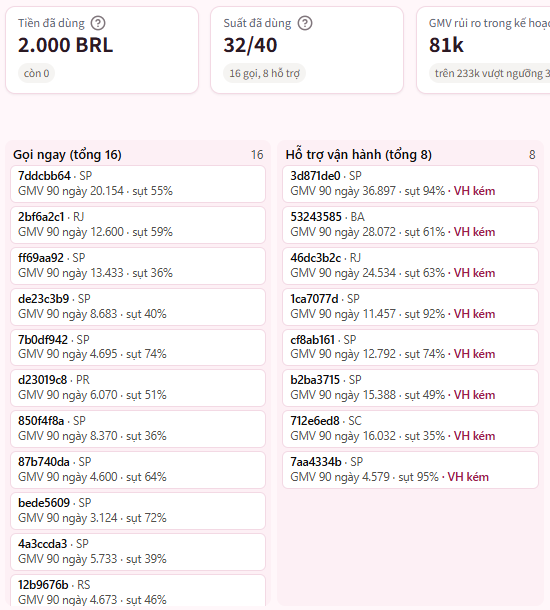
\includegraphics[width=0.47\textwidth]{image/app_7_crop_cols.png}}\hfill
\fbox{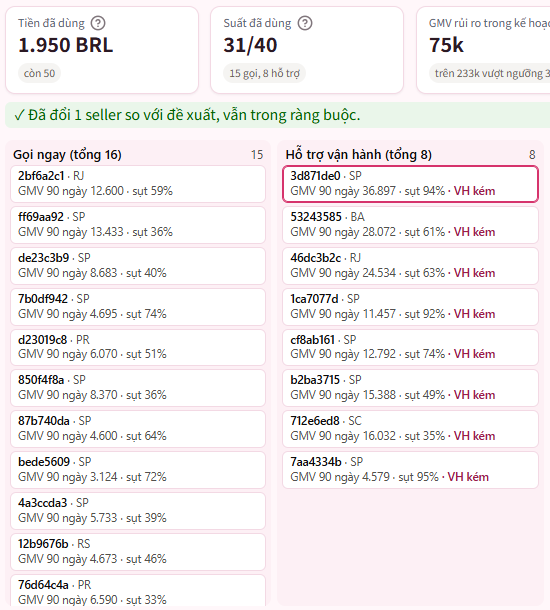
\includegraphics[width=0.47\textwidth]{image/app_8_crop_cols.png}}
\caption{Bảng kế hoạch mốc 01/03/2018 trước (trái) và sau (phải) khi kéo seller \texttt{7ddcbb64} khỏi cột \texttt{CALL}: tiền đã dùng giảm từ 2.000 xuống 1.950 BRL, số suất từ 32 xuống 31, và thanh xác nhận báo kế hoạch vẫn trong ràng buộc}
\label{fig:ui_drag}
\end{figure}

\appimage[0.7\textwidth]{image/app_9_bang_vuot_rang_buoc.png}{Cảnh báo khi thao tác tay vượt ngân sách (mốc 01/03/2018): nút Chốt kế hoạch bị khóa}{fig:ui_violate}

\appimage{image/app_5_kiem_chung.png}{Luồng A, bước 4 -- Kiểm chứng trên các tháng đã biết kết quả}{fig:ui_validation}

\appimage{image/app_4_whatif_tuyen.png}{Luồng B -- What-if hẹn giao theo tuyến}{fig:ui_whatif}


\end{document}
